\documentclass[reprint,amsmath,amssymb,aps,prx,superscriptaddress]{revtex4-2}

\usepackage{graphicx} % remove 'demo' option in real document
%\usepackage{times}
\usepackage{caption}
\captionsetup{justification   = raggedright,
              singlelinecheck = false}
              


\usepackage{chemfig}
\usepackage{graphicx}
\usepackage{amsmath, amsthm}
\usepackage{hyperref}
\usepackage{pgfplots} 
\usepackage[FIGTOPCAP]{subfigure}
\usepackage{array}

\pgfplotsset{compat=1.3} 
\pgfplotsset{every axis/.append style={font=\huge}}
\pgfplotsset{every tick label/.append style={font=\Large}}

\input{Headers/matlabdefault_colormap.tex}
\usepackage{graphicx}
\usepackage{amsmath, amsthm}
\usepackage{hyperref}
\usepackage{booktabs}
\usepackage{fullpage}
\usepackage{mathtools}
\usepackage{tikz-cd}
\usepackage{CJK} 
\usepackage[T1]{fontenc}
\usepackage[utf8]{inputenc}
%\usepackage{authblk}
\usepackage{appendix}
\usepackage{caption}
\usepackage{tikz}
\usetikzlibrary{arrows}
\usepackage{multirow}
\usepackage{dcolumn}% Align table columns on decimal point
\usepackage{bm}
\usepackage[export]{adjustbox}
\usepackage[misc]{ifsym}

% Macros file for Math 311 TeX files



\newcommand\Q{{\mathbf Q}}
\newcommand\R{{\mathbf R}}
\newcommand\C{{\mathbf C}}
\newcommand\T{{\mathbf T}}
\newcommand\Z{{\mathbf Z}}
\newcommand\N{{\mathbf N}}
\newcommand\UHP{{\mathcal H}}
\newcommand\Proj{{\mathbf P}}
\newcommand\Rsphere{{\widehat{\mathbf C}}}
\newcommand\lra{\longrightarrow}
\newcommand\lreq{\overset\sim\lra}
\newcommand\normal{\lhd}
\newcommand\Adj{\text{Adj}}
\newcommand\Aut{\text{Aut}}
\newcommand\Id{\text{Id}}
\newcommand\Ad{\text{Ad}}
\newcommand\ad{\text{ad}}
\newcommand\End{\text{End}}
\newcommand\g{{\mathfrak{g}}}
\newcommand\p{\mathbf p}
\newcommand\pdr{{p_d^R}}
\newcommand\pdw{{p_d^W}}
\newcommand\pu{{p_u}}
\newcommand\pb{{p_b}}
\newcommand\pd{{p_d}}
\newcommand\ppd{{\bar{p}_d}}
\newcommand\ppdw{{\bar{p}_d^W}}
\newcommand\ppdr{{\bar{p}_d^R}}


\newcommand\om{\omega}

\newcommand\hu{\hat{u}}

\newcommand\E{\mathbb{E}}


\newcommand\all{\forall}
\newcommand\F{\mathbb{F}}

\newcommand\e{\epsilon}

\newcommand\x{\mathbf x}
\newcommand\bu{\mathbf \mu}
\newcommand\y{\mathbf y}



\newcommand\Si{\Sigma}

\renewcommand{\Re}[1]{{\rm Re}\left(#1\right)}
\renewcommand{\Im}[1]{{\rm Im}\left(#1\right)}

\theoremstyle{plain}
\newtheorem{thm}{Theorem}[section]
\newtheorem{lemma}[thm]{Lemma}
\newtheorem{cor}[thm]{Corollary}
\newtheorem{prop}[thm]{Proposition}
\newtheorem{defn}[thm]{Definition}
\newtheorem{prob}[thm]{Problem}
\newtheorem{assum}[thm]{Assumption}
\newtheorem{result}[thm]{Result}


\theoremstyle{definition}
\newtheorem{remk}[thm]{Remark}
\newtheorem{fact}[thm]{Fact}

\theoremstyle{remark}
\newtheorem{ex}[thm]{Example}

\newcommand\cmat[4]{\left[\begin{array}{cc}#1&#2\\#3&#4\end{array}\right]}
\newcommand\rmat[4]{\left[\begin{array}{rr}#1&#2\\#3&#4\end{array}\right]}

\newcommand\cvec[2]{\left[\begin{array}{c}#1 \\ #2\end{array}\right]}

\newcommand\sumstack[2]{
\substack{
#1\\
#2}
}

\newcommand\tristack[3]{
\substack{
#1\\
#2\\
#3}
}

\newcommand\quadstack[4]{
\substack{
#1\\
#2\\
#3\\
#4}
}

\newcommand\eyej{
\substack{
i\\
i\neq j}
}

\newcommand\eyek{
\substack{
i\\
i\neq k}
}


%\newcommand\ol{\overline}

\include{xy}
\xyoption{all}
\SelectTips{cm}{}
\CompileMatrices

\include{epsf}
\newcommand{\graphillus}[3]{\epsfysize=#1truein
\vbox{\centerline{\epsffile{#2.eps}}\caption{#3}}}

\newcommand{\specialillus}[4]{\epsfysize=#1in
	\vbox{\centerline{\epsffile{#2.eps}}
		\kern -#1in \kern-1bp
                \epsfysize=#1in
		\centerline{\epsffile{#3.eps}}
		\kern1bp
		\caption{#4}}
	}







\newcommand\hvec[4]{\left[\begin{array}{cc}#1&#2\\#3&#4\end{array}\right]}
\newcommand\kpd{{k'_D}}
\newcommand\kpc{{k'_C}}
\newcommand\lpd{{l'_D}}
\newcommand\lpc{{l'_C}}
\newcommand\kd{{k_D}}
\newcommand\kc{{k_C}}
\newcommand\ld{{l_D}}
\newcommand\lc{{l_C}}
\newcommand\sone{{{\sum}_1}}
\newcommand\stwo{{{\sum}_2}}
\newcommand\wpp{{\omega_p}}
\newcommand\edp{{e^{-\delta_p}}}
\newcommand\ed{{e^{\delta}}}
\newcommand\eei{{e^{\epsilon_i}}}
\newcommand\ee{{e^{\epsilon}}}
\newcommand\wi{{w_i}}
\newcommand\ldk{w_Pe^{\epsilon_P+\gamma}}
\newcommand\eps{\epsilon}
\newcommand\del{\partial}
\newcommand\mL{\mathcal{L}}
\newcommand\proj{{\rm proj}}
\newcommand\vol{{\rm vol}}
\newcommand\adj{{\rm adj}}
\newcommand\norm[1]{\left\lVert#1\right\rVert}
\newcommand\Sig{\Sigma}
\newcolumntype{C}[1]{>{\centering\arraybackslash}p{#1}}
\newcommand\oom{\omega}
\newcommand\gam{\gamma}
\newcommand{\la}{\langle}
\newcommand{\ra}{\rangle}
\newcommand{\ton}{\text{on}}
\newcommand{\toff}{\text{off}}
\newcommand\epp{{e^{\epsilon_p}}}
\newcommand\epl{{\epsilon_p}}
\newcommand\eil{\epsilon_i}
\newcommand\sij{{\mathcal{L}^{i,j}}}
\newcommand\volp[1]{{\vol(P(#1))}}


\begin{document}

\title{Geometric Requirements for Nonequilibrium Discrimination}
\author{Gaurav G. Venkataraman}
\email{Correspondence:  gauravvman@gmail.com or dj333@cam.ac.uk}
\affiliation{Wellcome/CRUK Gurdon Institute, University of Cambridge.\\Tennis Court Rd, Cambridge, CB2 1QN, UK.}
\affiliation{Division of Medicine, University College London.  London WC1E 6BT, UK.}

\author{Eric A. Miska}
\affiliation{Wellcome/CRUK Gurdon Institute, University of Cambridge.\\Tennis Court Rd, Cambridge, CB2 1QN, UK.}
\affiliation{Department of Genetics, University of Cambridge.  Downing Street, Cambridge CB2 3EH, UK.}
\affiliation{Wellcome Sanger Institute, Wellcome Genome Campus, Cambridge CB10 1SA, UK.}

\author{David J. Jordan}
\email{Correspondence: gauravvman@gmail.com or dj333@cam.ac.uk}
\affiliation{Wellcome/CRUK Gurdon Institute, University of Cambridge.\\Tennis Court Rd, Cambridge, CB2 1QN, UK.}
\affiliation{Department of Genetics, University of Cambridge.  Downing Street, Cambridge CB2 3EH, UK.}

\begin{abstract}

We study: necessary conditions for the steady-state occupancies of multistep networks to achieve high sensitivity via thermodynamic drive; the ability of these networks to toggle between outputs by adjusting the amount of drive; the possible implementation of this dissipation-driven output toggling in the biochemical context of RNA granules.  In general, sensitivity allows the ratios of non-equilibrium steady states to depart far from their equilibrium limit, known as discrimination.  Discrimination is crucial for high fidelity information processing at the molecular scale, where steady-state occupancies correspond to (competing) products of biochemical reactions.  We define an analytically tractable measure on network discrimination schemes, termed orthogonality, which measures the extent to which discrimination is local.  The central proposition of our paper is that discrimination is fundamentally constrained by orthogonality.  We demonstrate that discrimination which amplifies binding energy differences requires low orthogonality, whereas discrimination which amplifies activation energy differences requires high orthogonality.  Subject to orthogonality requirements, {\it both} types of discrimination are maximized by maximizing dissipation.  Dissipation itself can drive orthogonality up or down. When increasing thermodynamic drive conflicts with orthogonality requirements, discrimination is non-monotonic.  We find that, due to its effect on orthogonality, modulating thermodynamic drive alone can sharply select between products which are favored by different energy types, without network fine-tuning.  Biologically, this corresponds to the ability to select between products by driving a single reaction type.  We consider this possibility in the context of liquid-liquid phase separated collections of RNA and protein known as granules, which appear to have precisely the structure required to tune orthogonality via adjusting the rate of ATP hydrolysis.

%We study multistep networks capable of product discrimination inspired by biological \emph{proofreading} mechanisms.   These networks expend free-energy to reach nonequilibrium steady states in which ratios of state occupancies are far from their equilibrium limit.  We introduce a measure on such nonequilibrium systems called orthogonality and show that it provides necessary conditions for proofreading.  In proofreading networks that discriminate with activation energy differences, called kinetic discrimination, this is the limit of high orthogonality. In networks that discriminate with binding energy differences, called energetic discrimination, it is the limit of low orthogonality.  We show that in both kinetic and energetic discrimination, minimum error requires maximizing dissipation in the appropriate orthogonality limits and show how this can lead to non-monotonic behavior in the error-rate as a function of the systems free-energy expenditure.  In addition, we show that in high orthogonality networks there are multiple directed paths to the product state.  In contrast, low orthogonality networks have, in general, a single dominant path to the product.  Finally, we introduce mixed networks, in which one product is favored energetically and the other kinetically.  In such networks, sensitive product switching can be achieved by increasing the free-energy expenditure across a single type of reaction.
\end{abstract}

\maketitle

\section{Introduction}
Systems driven out of thermodynamic equilibrium are capable of demonstrating extraordinarily varied behaviors.  One such behavior is enhanced discrimination: the ratio of nonequilibrium steady-state occupancies can deviate far from what is allowed by their energetic differences alone.  The cost of this flexibility is parametric complexity.  Nonequilibrium steady-state occupancies will generally depend on the system's full parametric details.

Enhanced discrimination is particularly important in a biological context, where biochemical reactions achieve extraordinary fidelity by discriminating between competing substrates having only marginally different equilibrium energies.  For example, equilibrium energy differences between nucleotides competing in a DNA replication reaction predict replication error rates of $\sim10^{-4}$; but observed rates are $\sim10^{-9}$.  To resolve this discrepancy, Hopfield \cite{Hopfield1974} and Ninio \cite{Ninio1975} proposed a network which uses non-equilibrium drive to enhance discrimination by amplifying equilibrium energy differences.  Such networks have been analyzed extensively, extended \cite{Ehrenberg1980,Murugan2012} and generalized \cite{Murugan2014}.

The Hopfield-Ninio scheme achieves its minimum error rate in the slow, quasi-adiabatic regime.  Some years later, Bennett introduced a discrimination scheme which achieves its error minimum in the fast, high-dissipation limit \cite{Bennett1979,Bennett1982}.  An essential difference between these schemes was only recently noted: quasi-adiabatic discrimination amplifies {\it binding energy} differences, whereas high-dissipation discrimination amplifies {\it activation energy} differences.  The two regimes were termed {\it energetic} and {\it kinetic} discrimination (respectively), and argued to be alternate in any single reaction step \cite{Sartori2013}.

We study the general requirements for non-equilibrium discrimination from a geometric perspective.  To this end, we introduce a measure on non-equilibrium systems, called {\it orthogonality}. The measure tightly bounds the degree to which a network's discrimination can be accurately represented by the transition rates near (0-2 links away from) the discriminatory nodes.  We find that local (high orthogonality) discrimination relies on the existence of many effective pathways directed towards the discriminatory nodes.  In contrast, discrimination schemes that depend on global network parameters (low orthogonality) are characterized by having a single dominant path towards the discriminatory nodes.

We show that high orthogonality networks are necessary for kinetic discrimination, whereas low orthogonality networks are necessary for energetic discrimination.  Subject to these orthogonality requirements, {\it both} kinetic and energetic discrimination increase with respect to dissipation.  When the orthogonality requirement conflicts with the dissipation requirement - which can happen in either discriminatory regime - the level of discrimination is non-monotonic with respect to dissipation.  This phenomena is responsible for the non-monotonicity observed in the original Hopfield-Ninio scheme.

We further show that orthogonality can be modulated by changing the drive of a single reaction type in an otherwise fixed network.  Whether dissipation increases or decreases orthogonality depends on whether it is used to drive reactions which increase or decrease the number of effective pathways towards the discriminatory nodes.  By shifting orthogonality, nonequilibrium drive can achieve simple, highly tunable selection between products which are favored by different energy types.

Hopfield noted that the reaction topologies necessary for energetic discrimination appear ubiquitously in biology.  Our results demonstrate how these molecular discrimination mechanisms can explore alternative product spaces by spending energy to transition to the kinetic regime, without cost to their original fidelity.  The degree to which a network can be repurposed in this manner is given by the degree to which its orthogonality can be modulated.  We consider this repurposing proposition in the particular case of localized collections of RNA and protein known as {\it granules} \cite{Brangwynne2009}, whose features bear all of the hallmarks of dissipation-driven orthogonality tuning.

\section{Definition of Orthogonality}
We consider systems whose dynamics are described by continuous time Markov chains.  System states and transitions can be represented as a fully connected directed graph (Figure 1(a)), and have dynamics represented by a matrix differential equation known as the Master equation
\[
\frac{d{p}}{dt} = \mL{p}
\]
where $\mL$ is a {\it Laplacian matrix} encoding the transition rates $k_{ij} = (j\to i)$ of the network in its off-diagonal elements, and having diagonal elements set such that all columns sum to zero:
\[
\mathcal{L}_{ij} =
 \begin{cases}
       {k_{ij}} & i\neq j, \ k_{ij}\ge0\\
       {-\sum_j k_{ij}} & i=j,\\
\end{cases}
\]
and ${p}$ is an $n$ dimensional vector representing the dynamic occupancy of the network states.

We require our systems to be fully-connected\footnote{Fully-connected graphs are ones in which it is possible to (not necessary directly) get from every state to every other state}, which implies that they have a single unique steady state (Appendix \ref{app:orth}).  Let $\rho$ be the vector of {\it steady states} of the Master equation determined by solving $\mL \rho=0$.  The degree to which a network {\it discriminates} between state $i$ and $j$ is given by the ratio of corresponding steady state elements: $\rho_i/\rho_j.$

In general, for systems both in and out of equilibrium, $\rho_i/\rho_j$ will be depend on transition rate parameters arbitrarily far from the discriminatory nodes $i, j.$  We aim to determine in which cases the ratio $\rho_i/\rho_j$ is more `local'.

By considering the geometry of the steady-state solution space, we can compute that (Appendix \ref{app:orth}):
\begin{equation}\label{ratio}
\frac{\rho_i}{\rho_j} = \frac{\norm{v_i - \proj_\sij(v_i)}}{\norm{v_j - \proj_\sij(v_j)}}.
\end{equation}
where: $v_i$ represents the $i$th column of $\mL;$ $\proj_\sij(v_i)$ denotes the projection of vector $v_i$ onto the $n-2$ dimensional subspace spanned by the columns of $\mL$ remove $i,j.$

In general, computing the subspace projections $\proj_\sij(v_i)$ will require orthogonalizing the columns of $\sij.$ From the perspective of Equation \ref{ratio}, this (recursive) orthogonalization procedure is the origin of global parametric complexity in $\rho_i/\rho_j$.

In the special case where the vectors that span $\sij$ are orthogonal, $\sij_{\text{orth}}$, the Equation \ref{ratio} projections can be simply computed:
\begin{equation}\label{proj}
\proj_{\sij_{\text{orth}}}(v_i) = \sum_{l\in \sij}\langle v_i, v_l \rangle v_i.
\end{equation}
Graphically, $\la v_i, v_l \ra\neq 0$ only if the $i$th and $l$th nodes on the digraph associated with $\mL$ are directly linked or direct arrows at one or more mutual nodes.  Therefore, $\sij_{\text{orth}}$ corresponds to the case in which $\rho_i/\rho_j$ depends on only transition rates 0-2 connections away from the nodes $i,j.$  The matrix $\sij$ having orthogonal columns implies {\it local} discrimination between states $i$ and $j$.

In practice, $\sij$ having purely orthogonal columns conflicts with our requirement that $\mL$ describe dynamics on a fully connected graph.  Distance of an $\sij$ matrix from the perfectly orthogonal case is the relevant quantity to consider.
To that end, we compute the difference between the true projection of a vector $v$ onto $\sij,$ $\proj_\sij(v),$ and the projection assuming that $\sij$ is orthogonal, $\proj_{\sij_{\text{orth}}}(v),$
\begin{equation}\label{orth_approx}
\begin{aligned}
&\norm{\proj_\sij(v) - \proj_{\sij_{\text{orth}}}(v)}\\
&= \norm{\sij(\sij^T\sij)^{-1}\sij^Tv - \sij\sij^Tv} \\
 &\le \norm{\sij(\sij^T\sij)^{-1}\sij^T - \sij\sij^T}\norm{v},\\
& = \norm{\mathbf{I} - \sij^T\sij}\norm{v}
\end{aligned}
\end{equation}
where the inequality is due to Cauchy-Schwartz and the final line is arrived at by simplifying the term in the first norm (Appendix \ref{app:proj}).

We define {\it orthogonality} to capture this distance.

\begin{defn}[Orthogonality]{We define the {\it orthogonality} of the discrimination between states $i$ and $j$ of network having Laplacian $\mL$ to be
\[
\Theta(\sij) = 1 - \norm{\mathbf{I} - \widehat{\sij}^T\widehat{\sij}}_F
\]
where $\norm{ \ }_F$ denotes the Frobenius norm and $\sij$ is a $(n \times n-2)$ matrix constructed by removing the columns corresponding to the $i,j$ discriminatory nodes from $\mL;$ and $\widehat{A}$ denotes the matrix $A$ having every column normalized to be of unit length.  Note that orthogonality is defined with respect to a network {\it and} two nodes of discriminatory interest.  We will use the term `discriminatory scheme,' to refer to this (network, nodes) pair and therefore refer to the `orthogonality of a scheme' leaving the specific discriminatory nodes $i,j$ implicit.
}
\end{defn}

Orthogonality can be understood to capture the number of effective pathways directed towards the discriminatory nodes.  To illustrate this, we consider discriminating between the end nodes of a 4 node toy model (Figure \ref{fig:toy_model}(a)) having bidirectional connections equal to either $k$ or $l$ (black, red, arrows in \ref{fig:toy_model}(a), respectively).  As the ratio $r=k/l$ grows, the black path becomes singly dominant over the red paths.  Correspondingly, the orthogonality decreases (Figure \ref{fig:toy_model}(b)) as $\Theta \sim O(r^{-2})$ (Appendix \ref{app:4node}).

Alternatively, we can ask: when does deleting the black links between the middle two nodes in Figure \ref{fig:toy_model}(a) affect orthogonality?  We find that when these arrows do not constitute part of a dominant path ($r\approx1$), deleting them has no effect on orthogonality.  But when these links {\it do} constitute part of a dominant path ($r>>1$), deleting them significantly increases orthogonality (Appendix \ref{app:4node}).

\pgfplotsset{yticklabel style={text width=5em,align=right}}
\begin{figure}[htb]

\resizebox{0.75\columnwidth}{!}{
\subfigure{
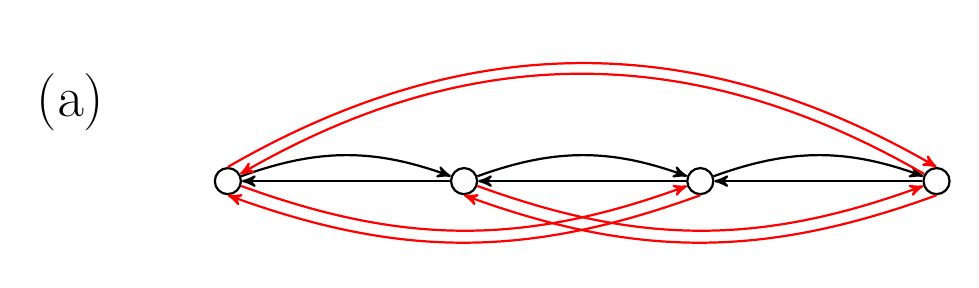
\begin{tikzpicture}[->,>=stealth',auto,node distance=3cm,
  thick,main node/.style={circle,draw,font=\sffamily\Large\bfseries}]
  \node[] at (-2,1) {\huge (a)};
\node[main node] (1) {};
\node[main node] (2) [right of=1] {};
\node[main node] (3) [right of=2] {};
\node[main node] (4) [right of=3] {};

\draw [->] (1) to [out=20, in=160] (2);
\draw [->] (2) to [out=20, in=160] (3);
\draw [->] (3) to [out=20, in=160] (4);
\draw [->] (2) -- (1);
\draw [->] (3) -- (2) ;
\draw [->] (4) -- (3);
\draw [->, red] (4) to [out=150,in=30] (1);
\draw [->,red] (1.north) to [out=30,in=150] (4.north);
\draw [->,red] (1) to [out=30,in=150, bend right=20] (3);
\draw [->,red] (3.south) to [out=150,in=30, bend left = 20] (1.south);
\draw [->,red] (2) to [out=30,in=150, bend right=20] (4);
\draw [->,red] (4.south) to [out=150,in=30, bend left = 20] (2.south);
\end{tikzpicture}}
}
\resizebox{0.76\columnwidth}{!}{
\subfigure{
\begin{tikzpicture}
\node[] at (-2,7) {\huge (b)};

\begin{axis}[%
%width=4in,
%height=4in,
%at={(0in,0in)},
scale only axis,
xmin=1,
xmax=10,
xtick={1,3,5,7,9},
xlabel style={font=\huge\color{white!15!black}},
xlabel={$r = k/l$},
ymin=0,
ymax=0.55,
ytick={0.1,0.3,0.5},
ylabel style={font=\huge\color{white!15!black}, at={(axis description cs:-0.15,0.5)}},
ylabel={$\Theta$},
axis background/.style={fill=white},
legend style={legend cell align=left, align=left, draw=white!15!black}
]
\addplot [color=black]
  table[row sep=crcr]{%
1	0.528595479208968\\
1.09090909090909	0.50147673688684\\
1.18181818181818	0.477019492251525\\
1.27272727272727	0.454895067403881\\
1.36363636363636	0.434816959975228\\
1.45454545454545	0.416537192638981\\
1.54545454545455	0.399841821547982\\
1.63636363636364	0.384546414763086\\
1.72727272727273	0.370491866810496\\
1.81818181818182	0.357540687167248\\
1.90909090909091	0.3455737869816\\
2	0.334487735353838\\
2.09090909090909	0.324192434963534\\
2.18181818181818	0.314609161188975\\
2.27272727272727	0.305668910853743\\
2.36363636363636	0.297311012007194\\
2.45454545454545	0.289481952467273\\
2.54545454545455	0.282134391129488\\
2.63636363636364	0.275226321781979\\
2.72727272727273	0.268720364185128\\
2.81818181818182	0.262583161453856\\
2.90909090909091	0.256784866374109\\
3	0.251298702273067\\
3.09090909090909	0.24610058653295\\
3.18181818181818	0.241168806873832\\
3.27272727272727	0.236483742205569\\
3.36363636363636	0.232027621226193\\
3.45454545454545	0.227784313077425\\
3.54545454545455	0.223739145301524\\
3.63636363636364	0.219878745113962\\
3.72727272727273	0.216190900643201\\
3.81818181818182	0.212664439316352\\
3.90909090909091	0.209289121007604\\
4	0.206055543930894\\
4.09090909090909	0.202955061562617\\
4.18181818181818	0.19997970913475\\
4.27272727272727	0.197122138452283\\
4.36363636363636	0.194375559968448\\
4.45454545454546	0.191733691202618\\
4.54545454545454	0.18919071071374\\
4.63636363636364	0.186741216950604\\
4.72727272727273	0.184380191392375\\
4.81818181818182	0.182102965471274\\
4.90909090909091	0.179905190836244\\
5	0.177782812573782\\
5.09090909090909	0.175732045051198\\
5.18181818181818	0.173749350089879\\
5.27272727272727	0.171831417212448\\
5.36363636363636	0.16997514573921\\
5.45454545454545	0.168177628536371\\
5.54545454545455	0.166436137242153\\
5.63636363636364	0.164748108817365\\
5.72727272727273	0.163111133284805\\
5.81818181818182	0.161522942537425\\
5.90909090909091	0.159981400108769\\
6	0.158484491811051\\
6.09090909090909	0.157030317156709\\
6.18181818181818	0.155617081488386\\
6.27272727272727	0.15424308875037\\
6.36363636363636	0.152906734841615\\
6.45454545454545	0.151606501496755\\
6.54545454545455	0.150340950647027\\
6.63636363636364	0.149108719217995\\
6.72727272727273	0.147908514325239\\
6.81818181818182	0.146739108833137\\
6.90909090909091	0.145599337245228\\
7	0.144488091897757\\
7.09090909090909	0.143404319430742\\
7.18181818181818	0.142347017513314\\
7.27272727272727	0.141315231802305\\
7.36363636363636	0.140308053114993\\
7.45454545454545	0.139324614798688\\
7.54545454545455	0.138364090281396\\
7.63636363636364	0.13742569078925\\
7.72727272727273	0.136508663217644\\
7.81818181818182	0.135612288144175\\
7.90909090909091	0.13473587797252\\
8	0.133878775197339\\
8.09090909090909	0.13304035078111\\
8.18181818181818	0.132220002634592\\
8.27272727272727	0.13141715419331\\
8.36363636363636	0.130631253083061\\
8.45454545454545	0.129861769868044\\
8.54545454545455	0.129108196875724\\
8.63636363636364	0.128370047093001\\
8.72727272727273	0.127646853128714\\
8.81818181818182	0.126938166237881\\
8.90909090909091	0.126243555403441\\
9	0.125562606471598\\
9.09090909090909	0.124894921337152\\
9.18181818181818	0.124240117175503\\
9.27272727272727	0.123597825718219\\
9.36363636363636	0.122967692569348\\
9.45454545454546	0.122349376559807\\
9.54545454545454	0.12174254913742\\
9.63636363636364	0.121146893790321\\
9.72727272727273	0.120562105501626\\
9.81818181818182	0.119987890233413\\
9.90909090909091	0.119423964438198\\
10	0.118870054596202\\
};
\end{axis}
\end{tikzpicture}}
}
%\resizebox{0.75\columnwidth}{!}{
%\subfigure{
%% This file was created by matlab2tikz.
%
%The latest updates can be retrieved from
%  http://www.mathworks.com/matlabcentral/fileexchange/22022-matlab2tikz-matlab2tikz
%where you can also make suggestions and rate matlab2tikz.
%
\definecolor{mycolor1}{rgb}{0.00000,0.44700,0.74100}%
%
\begin{tikzpicture}
%\node[] at (-2,7) {\huge (b)};

\begin{axis}[%
%width=4in,
%height=4in,
%at={(0in,0in)},
scale only axis,
xmin=0,
xmax=1,
xtick={0, 0.2, 0.4, 0.6, 0.8, 1},
xlabel style={font=\Large\bfseries\color{white!15!black}},
xlabel={Connectivity, 0=Grid},
ymin=-2.5,
ymax=0.5,
yticklabel style = {font=\Large},
ylabel style={font=\huge\bfseries\color{white!15!black}, at={(axis description cs:-0.15,0.5)}},
scale ticks below exponent=2,
ylabel={$\Theta$},
axis background/.style={fill=white},
legend style={legend cell align=left, align=left, draw=white!15!black}
]
\addplot [color=mycolor1, line width=2.0pt, draw=none, mark=square, mark options={solid, mycolor1}]
 plot [error bars/.cd, y dir = both, y explicit]
 table[row sep=crcr, y error plus index=2, y error minus index=3]{%
1	0.0158897932895343	0.0219638609519872	0.0219638609519872\\
0	-2.19152922410445	0.0442727133533317	0.0442727133533317\\
0.1	-1.26900238075602	0.113140127221996	0.113140127221996\\
0.2	-1.13717407560137	0.105399483670646	0.105399483670646\\
0.3	-1.00117652331271	0.088778703694582	0.088778703694582\\
0.4	-0.860142584690047	0.0752706537627627	0.0752706537627627\\
0.5	-0.726084325807173	0.0648688752958107	0.0648688752958107\\
0.6	-0.588945001891375	0.0557394993663173	0.0557394993663173\\
0.7	-0.444804928347819	0.0432954017554721	0.0432954017554721\\
0.8	-0.287006316742788	0.0332660232213172	0.0332660232213172\\
0.9	-0.132989953746229	0.0271438744901984	0.0271438744901984\\
};

\end{axis}

\end{tikzpicture}%
}
%}
\caption{Orthogonality captures the number of effective pathways directed at discriminatory nodes.  (a) A toy four-node discriminatory scheme.  (b) When each black and red arrow in panel (a) has weight $k, \ l$ (respectively) we find that the orthogonality ($\Theta$) decreases as the black arrows dominate, creating a singly dominant path.  Note that the $x$-axis begins at $r=1,$ corresponding to an all-to-all connected graph with equal weights.\label{fig:toy_model}}
\end{figure}


%As connections of equal order of magnitude are deleted from an all-to-all connected graph, orthogonality decreases.  For each graph, a fraction of nodes were randomly deleted; error bars represent standard deviation of orthogonality over 1000 trials at each sparsity. At 0 is $\Theta(Grid)$ 

Our example demonstrates that an all-to-all connected discrimination scheme ($r=1$) with equal rates has greater orthogonality than a line topology $(r>>1)$ having equal rates ($k$), for $N=4$ nodes.  We can compute that this holds for all $N$ (Appendix \ref{app:line_v_all}).  The increased orthogonality of the all-to-all relative to line topology captures a more general fact: orthogonality tends to decrease as connections are removed from a discrimination scheme, so long as these connections are of equal order magnitude to remaining connections.  We demonstrate this computationally (Figure~\ref{sfig:orth}). 

\section{Orthogonality in the Hopfield-Ninio Scheme}
We first demonstrate the relationship between orthogonality and discrimination using the classical Hopfield-Ninio scheme, shown graphically in Figure \ref{fig:hopfield}(a).  Here, substrates $S= \{W, \ R\}$ compete to form complexes with enzyme $E$.  `Wrong' and `Right' products are formed from substrates $R$ and $W$ (respectively), at rates proportional to the steady state occupancy of the final complex $\rho_{ES}.$  We thus define the {\it error fraction} achieved by the discrimination scheme to be
\[
\xi = \frac{\rho_{EW}}{\rho_{ER}}.
\]
\begin{figure*}[ht]
\subfigure[]{
 \resizebox{0.325\textwidth}{!}{
\schemestart
E\arrow(aa--bb){<=>[$k^{\prime}_R$][$k_R$]}[,,,red] $ER^*$
\arrow(--cc){<=>[$m'$][$m$]}[-90,,,red]$ER$
\arrow(@cc--@aa){<=>[$l^{\prime}_R$][$l_R$]}[,,,red]
\arrow(@aa--dd){<=>[$k_W$][$k^{\prime}_W$]}[180,,,red] $EW^*$
\arrow(--ee){<=>[${m'}$][${m}$]}[-90,,,red] $EW$
\arrow(@ee--@aa){<=>[$l_W$][$l^{\prime}_W$]}[,,,red]
\schemestop

}} 
\subfigure[]{
\resizebox{0.4\textwidth}{!}{
% This file was created by matlab2tikz.
%
%The latest updates can be retrieved from
%  http://www.mathworks.com/matlabcentral/fileexchange/22022-matlab2tikz-matlab2tikz
%where you can also make suggestions and rate matlab2tikz.
%
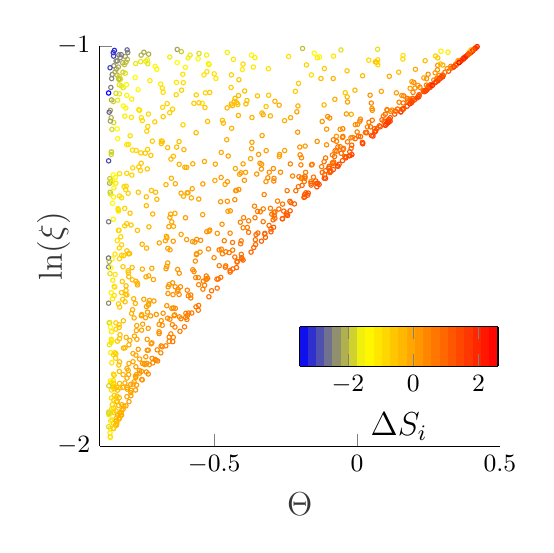
\begin{tikzpicture}[scale=1]

\begin{axis}[%
width=2in,
height=2in,
at={(0in,0in)},
scale only axis,
xmin=-0.9,
xmax=0.5,
xtick={-0.5,0,0.5},
xlabel style={font=\large\bfseries\color{white!21!black}},
xlabel={$\Theta$},
xticklabel style = {font=\small},
ymin=-2,
ymax=-1,
ytick={-2,-1},
ylabel style={font=\large\bfseries\color{white!21!black}, at={(axis description cs:-0.05,0.5)}},
ylabel={$\ln(\xi)$},
yticklabel style = {font=\small},
axis background/.style={fill=white},
axis x line*=bottom,
axis y line*=left,
legend style={legend cell align=left, align=left, draw=white!15!black}
colormap name=mymap,
colorbar sampled,
colorbar horizontal,
colorbar style={xlabel=$\Delta S_i$,
width=0.5*
\pgfkeysvalueof{/pgfplots/parent axis width},
at={(0.5,0.2)},anchor=south west,
font=\large,
xticklabel style = {font=\small},
}
]
\addplot[scatter, only marks, mark=o, mark size=0.7906pt, scatter src=explicit, scatter/use mapped color={mark options={}, draw=mapped color}] table[row sep=crcr, meta=color]{%
x	y	color\\
-0.85158714062712	-1.8506764826628	-0.70986693475978\\
-0.328479230208016	-1.17150394841944	-0.0992487284195959\\
0.201058024758192	-1.13458162987476	1.45135435157473\\
-0.131012492848958	-1.0268731053345	-1.36746621751927\\
-0.540268497163794	-1.42146557208882	0.0605577371951056\\
-0.848010907857566	-1.60236034475682	-0.894956935521254\\
-0.859306300629019	-1.85998190355987	-0.980209452825703\\
0.0523780814310758	-1.15619869352752	0.313856671404255\\
-0.842113511164757	-1.94581481027728	-0.374480331379608\\
-0.320569780696558	-1.47807665116216	1.107791375441\\
0.117037080383405	-1.16309327707161	0.547548973464419\\
-0.685190639809052	-1.6864472567039	0.273825405112862\\
-0.865367100368701	-1.69096752528199	-1.51394849064435\\
-0.843417614381916	-1.91229644933005	-0.532181959684083\\
-0.757834544043223	-1.31122174682874	-0.699783449981952\\
0.233948147926907	-1.07966342730552	0.0323559378213655\\
-0.851803919920382	-1.95607085120834	-0.59322968747566\\
-0.857773303956051	-1.9346308616399	-0.813609681583244\\
-0.865991552673622	-1.34287414550367	-2.10289981251752\\
0.282773083435289	-1.08013599660972	1.0739833738138\\
-0.755396246781458	-1.29303482378741	-0.606249722434317\\
-0.594662825762288	-1.36698148981732	-0.0821593927138918\\
-0.815407246308103	-1.3512687978577	-0.837247900503458\\
-0.413371543411392	-1.08422887808116	-0.556093452823776\\
-0.766210591980486	-1.10911172044903	-1.38352713893899\\
-0.660955336644194	-1.60177565415339	0.140385897694917\\
-0.663009064093536	-1.68031643590745	0.319126571129306\\
-0.809608486672494	-1.62067747112621	-0.42441612196479\\
-0.475073654495389	-1.5076395251864	0.442791273993199\\
-0.728304027985403	-1.451984257738	-0.272304959519939\\
-0.450754315487802	-1.27495418739477	0.0143937298736696\\
-0.773877703716112	-1.80176341672457	0.0692125399545731\\
-0.654817396204235	-1.42840678853869	-0.030796458182814\\
-0.271051075489934	-1.27088708617811	0.131402300891437\\
-0.339651713535607	-1.29311592574185	0.231800142643147\\
-0.555478908693049	-1.57889488988294	0.49110991269759\\
-0.622819330543413	-1.23891310075176	-0.435811323201957\\
-0.733822983353054	-1.03445770171761	-1.60355228173951\\
-0.0776146017586115	-1.13310757624443	-0.0946906941391082\\
-0.804358870523215	-1.85335085699519	-0.091011490621065\\
0.399690284855534	-1.01444335020919	1.03035932014725\\
-0.561749760754416	-1.51924116102649	0.27014966978848\\
-0.523059267616168	-1.58045040789798	0.589551730932461\\
-0.775807151863453	-1.64341487265836	-0.207551515416074\\
-0.753717217003296	-1.67113169441541	-0.0960807838982745\\
-0.600674402264712	-1.05309958306949	-1.25326154792467\\
0.28767813022425	-1.08279189605009	1.29371784433353\\
-0.816583738700049	-1.52389995962056	-0.621479076769321\\
-0.73858676315377	-1.57699068649275	-0.0980163635471155\\
-0.242989277869637	-1.42333661891652	1.28960565737079\\
-0.0072734802854415	-1.11028585902782	-0.310191959402642\\
-0.726583338514677	-1.79633498658462	0.282758243458926\\
-0.842543054986283	-1.88948295814351	-0.503374896842337\\
-0.609879051921266	-1.07061322869254	-1.02023533895223\\
-0.56360529413849	-1.65191612934039	0.644214757593038\\
0.346618911588103	-1.04764366230693	2.10764092467587\\
0.394350214236771	-1.01771219208712	0.958668931813346\\
-0.538054144236078	-1.58790718350681	0.52108998958683\\
-0.776340602282282	-1.07883339898714	-1.41878562493126\\
-0.1833196294451	-1.37702004550041	1.19956326666418\\
0.185525438441433	-1.13256593112859	0.725781729370534\\
-0.851973374561101	-1.025017213232	-2.93803863729592\\
-0.753944090964895	-1.71014490914826	0.0246025587084165\\
0.298646025935978	-1.0766798182782	1.7809765700925\\
-0.775349942657986	-1.85984467208235	0.15610163355549\\
0.0411540875867533	-1.03542332652928	-0.858593358102547\\
-0.849090645685093	-1.01092113358308	-3.16152201133102\\
0.134159198749176	-1.16245626881707	1.04927205413829\\
-0.817545501973263	-1.75496917985141	-0.387735942671936\\
0.191103902522848	-1.14137930727194	1.51948671337821\\
-0.616136053911544	-1.68165697985684	0.546488240845131\\
-0.578294555823483	-1.66724205458512	0.627107992193465\\
0.365761240120544	-1.03563948466925	1.3114403238939\\
-0.59549734337557	-1.68340610826243	0.636107199674588\\
-0.836574658521727	-1.40630198224887	-1.01670145641255\\
-0.0821588271380274	-1.02511912062921	-1.05422788399541\\
-0.183331867639389	-1.37124488552985	1.10271343601172\\
-0.7897201590507	-1.17837230748728	-1.03142417717729\\
-0.52588484335148	-1.46406485055932	0.269459885871527\\
0.101134207190413	-1.18794682223983	1.18142511796284\\
-0.0587411087365679	-1.25159380283383	0.596899428398601\\
-0.307090085147514	-1.31546269180847	0.238890428352816\\
0.0641550779809238	-1.0393235021577	-0.580212773050436\\
-0.115307494707253	-1.28912921975911	0.686058752401918\\
0.072414296798095	-1.03456503143457	-0.836894704746709\\
-0.643073132725057	-1.72830485237674	0.531947135944541\\
0.231732593715291	-1.11191375419323	1.11589890203997\\
-0.833486644045845	-1.02187735391371	-2.47883806420313\\
-0.55455697055535	-1.64845337065933	0.673053948655103\\
-0.765793019307991	-1.75811651994097	0.0542499063247774\\
-0.687069938090055	-1.0950782781644	-1.11765989839373\\
-0.239452860670647	-1.02604283707799	-0.972121946670648\\
-0.0552528106394876	-1.26808414744047	0.871019943544123\\
-0.729256603768436	-1.57446042184561	-0.165735917920378\\
-0.324947576216237	-1.37125396686202	0.500524630746049\\
-0.293809823283773	-1.43450417512118	0.857315065786462\\
-0.590470785739191	-1.62430645020736	0.466080636773424\\
-0.808482714617454	-1.04030053354668	-1.93523370318136\\
-0.753454656019991	-1.83352405209525	0.233941089395793\\
-0.61403597295967	-1.11025121662331	-0.726238702929849\\
-0.717251580869541	-1.78069752954602	0.332672084285109\\
-0.599082155630435	-1.66804726068076	0.545795681217498\\
0.0100578890737656	-1.18769039452353	0.661657576171805\\
-0.408214887670969	-1.44044927916464	0.525204993204603\\
-0.707783032361183	-1.18949724004296	-0.712355589821155\\
-0.42579132850682	-1.3062049551487	-0.0819651926085603\\
-0.818262638932694	-1.10362627490077	-1.62773154666532\\
-0.869469197469334	-1.28694642135	-2.8845477228542\\
-0.642639139898044	-1.27553972555734	-0.450191281301402\\
0.0471074224514688	-1.2018911152283	0.842391141666333\\
-0.86020308907759	-1.61665616907611	-1.24548771624143\\
-0.842389940226129	-1.05732121357359	-2.14606424335288\\
-0.602652217053508	-1.30305149722332	-0.182554037770831\\
-0.309361782985159	-1.12293575144531	-0.562593369238747\\
-0.860918792430138	-1.74114961283069	-1.18506081082584\\
-0.859261461695068	-1.84121054629743	-1.01146976664201\\
-0.71800646274834	-1.74195931339297	0.195078265781934\\
-0.0270146024249589	-1.27444770207386	1.3654008904423\\
0.011702342823708	-1.18272350421277	0.469351342637949\\
-0.794435706691934	-1.41785960692962	-0.527239332921769\\
-0.23258829549812	-1.17900932314266	-0.082576641269786\\
-0.517596495573178	-1.04595869772391	-1.1605944803711\\
-0.123916447088792	-1.30145445974045	0.665124956068146\\
-0.804704547468499	-1.00963679678218	-2.67775780474562\\
-0.402937700508806	-1.53234802821825	0.942171632985386\\
-0.858234480783436	-1.73676749200633	-1.05822428455224\\
-0.803836074878931	-1.03326618985796	-2.01383817866107\\
-0.744709098703871	-1.793572477413	0.152172702056617\\
-0.823986283494814	-1.37916823408499	-0.878530701427515\\
-0.421815121425775	-1.55379425319188	0.951075690918803\\
-0.292832870761605	-1.30621418232501	0.400998566098245\\
-0.179126532637248	-1.36694707609765	1.10623425216267\\
-0.440132468798958	-1.14481456554919	-0.285002489275421\\
0.41714374763737	-1.003501256323	0.453520457154561\\
-0.427156294254775	-1.13086393867465	-0.464232816965047\\
-0.632203991217543	-1.0907469203945	-1.09591569918492\\
-0.0214634464160437	-1.22929649537235	0.509691036382733\\
-0.638310577516708	-1.67195660155453	0.338978866318211\\
-0.81212881603366	-1.75430476642087	-0.326646146751378\\
-0.706458783433504	-1.78356898493657	0.390139313479355\\
-0.864875503330233	-1.33139348598029	-1.94191397862433\\
-0.662751057053618	-1.25389535802744	-0.442310424937582\\
-0.832121959102366	-1.09694414931445	-1.68669900905859\\
-0.665898054676884	-1.55077902533179	0.0890931668702226\\
-0.839163318553017	-1.48611772628599	-0.958247362498855\\
-0.287283802106032	-1.13812001722543	-0.234127059699533\\
-0.856358045555727	-1.8962634762278	-0.810629872045347\\
-0.443597655441875	-1.411905693737	0.275388484829072\\
-0.740332791570607	-1.6790224346022	0.0277779610148458\\
-0.348406469186352	-1.1245808152339	-0.465912056384577\\
-0.0720577381896428	-1.22567505153679	0.120145599193737\\
-0.591214252367395	-1.02960329947305	-1.51200996347865\\
-0.273563984258397	-1.40735812540824	0.872758436342069\\
-0.655317292911084	-1.02743486219131	-1.58209541345775\\
0.387708315488738	-1.02202396155965	1.16523471101033\\
0.0720531778240421	-1.00804334500104	-1.68602040583824\\
-0.737437819372352	-1.39909275612211	-0.397176317507857\\
-0.246527902567852	-1.41738136994476	1.0903456030244\\
-0.081471369730195	-1.28980604173457	0.797486103812908\\
-0.334565060936005	-1.48776909931872	1.06227780281142\\
0.0198776474146605	-1.24185644233362	1.23199668914471\\
-0.584319508259996	-1.0225180304639	-1.60752404251705\\
0.0291406551154648	-1.21623128654955	0.844691519652136\\
0.40775647363444	-1.00859794692971	-0.267357215954204\\
-0.662488415894717	-1.54223451630458	0.0405326492725293\\
-0.312093874482538	-1.32926846480521	0.407432003229985\\
-0.718156885901727	-1.55566064217138	-0.0486717166322946\\
-0.637280199004463	-1.41833015009242	-0.0754548158558363\\
-0.565941907808555	-1.53757214532915	0.33067120670657\\
0.374914638654648	-1.02904477690122	0.882574860403626\\
-0.817780414205874	-1.68684555476241	-0.459464863077388\\
0.213425326324076	-1.09844319212393	0.151325376757452\\
-0.608975434452666	-1.19694495419466	-0.764392034603904\\
-0.355811382249274	-1.4841451342698	0.868594921449838\\
-0.763567894384184	-1.3021541799101	-0.595256128900761\\
-0.862243826874255	-1.7664623682896	-1.22652475775671\\
-0.692164248604738	-1.49222689007577	-0.0447442630498203\\
-0.841923216035165	-1.94781510086467	-0.366594258485832\\
-0.307788767665114	-1.44844787575945	0.91360168872143\\
0.300829039194579	-1.07392264705883	1.22162294202705\\
-0.615597270889084	-1.47083928917113	-0.0340002077827199\\
-0.358719194674404	-1.40029865833163	0.535973636402392\\
-0.338535445993134	-1.41428802214773	0.634551805731889\\
-0.600376181788933	-1.42921882326346	0.117540041585623\\
-0.720739257684435	-1.74435828908051	0.254433413645375\\
-0.518302692418207	-1.62679246555679	0.775276742870149\\
0.0941858487294988	-1.18848294422822	1.10220155880654\\
-0.681630759461273	-1.69806794126079	0.262613063742763\\
-0.700489981309189	-1.38320303935771	-0.322839537617581\\
0.116542062854491	-1.17918041968412	1.32367107516972\\
-0.772971447353725	-1.82187843789406	0.0762184404312739\\
-0.863409351015725	-1.97691613705301	-0.977433063108533\\
-0.838491002946665	-1.88843620318608	-0.4323233272313\\
-0.396880094899792	-1.42901772316758	0.553392183558155\\
0.0684856629381809	-1.04057798612046	-0.436709561596409\\
0.195977472707065	-1.11590232426285	0.480571980015971\\
-0.172950423940295	-1.37277027103453	1.30228456419723\\
-0.686472124098344	-1.76707565775493	0.422532019074566\\
0.0921401182984307	-1.17470794382477	0.653451620422537\\
-0.780190137360242	-1.67967627494092	-0.192381392929934\\
-0.574909200362896	-1.29427354422816	-0.172467761187207\\
-0.636467278200552	-1.60183151446268	0.250897749348792\\
-0.424596198052378	-1.361280937814	0.352637678930552\\
-0.820327510191759	-1.04182224387766	-2.11013144731906\\
-0.654929402417648	-1.68293408477037	0.379584778155459\\
-0.81116529021212	-1.02606942779971	-2.15032527654314\\
-0.115353265399078	-1.14719612645171	-0.291677109044599\\
-0.567355828537043	-1.49000692272604	0.200896910691931\\
-0.042507385925679	-1.27621940001607	1.01255705610903\\
0.160348670310939	-1.03235788480848	-0.86301481121832\\
-0.732470038160959	-1.04430229647808	-1.63604105599108\\
0.29971336726555	-1.07613994551205	2.04455739590286\\
-0.0387215150589451	-1.27739175198173	1.25741271982082\\
-0.844384795249284	-1.94689966602691	-0.416986500475823\\
-0.517481224167964	-1.46267948602661	0.256190000497492\\
-0.152347585507026	-1.32752921811183	0.77621488961142\\
-0.824419283645584	-1.61619864810237	-0.599792421821286\\
-0.857256998712996	-1.53211482295552	-1.25049169418251\\
-0.781639977837005	-1.6317450701404	-0.228426275486696\\
0.215465876664725	-1.1269803408491	1.79130897081298\\
0.259041794668694	-1.09663739275973	1.07852795313569\\
0.00495751903770003	-1.22535817598157	0.867654431577559\\
-0.855496625686269	-1.33969654490036	-1.46737601084096\\
0.248855712738256	-1.07053094844573	0.350805411623816\\
-0.47527959771476	-1.26578598512951	-0.12411926889369\\
0.0535041765845784	-1.16065564436823	0.313721833055427\\
0.0704647829460134	-1.20561253972354	1.20954830172781\\
-0.29827413438303	-1.4203028392348	0.772164065072108\\
0.248896428360701	-1.0998094379025	0.812685387169526\\
0.00192268191732825	-1.19562525045202	0.43286911119749\\
-0.541901760306464	-1.1431249991281	-0.983567265459332\\
-0.109791725310323	-1.31159560158745	1.01713048142166\\
0.153366117864329	-1.16476067345542	1.78106886343528\\
-0.629241918867499	-1.00842294647476	-2.17474842102862\\
-0.824221246005196	-1.52310592047184	-0.7043726841194\\
0.335965006946981	-1.05340730920607	1.57068826358123\\
-0.379274906064834	-1.43685715821969	0.603368456101449\\
-0.470942611893912	-1.51926994264753	0.483595752990422\\
-0.0670158801916851	-1.25204028321853	0.757884608549082\\
-0.852378293829732	-1.82009985416339	-0.82177413137163\\
0.245936703059987	-1.10691835665162	1.31203319550965\\
-0.869581452627582	-1.64277673900595	-2.35447618434345\\
0.0418068788417337	-1.19046548924684	0.627912525948636\\
-0.210676646084265	-1.16431840138532	0.0275031662105569\\
0.137764015327085	-1.11701435959569	0.0953248610984193\\
-0.706754531740645	-1.05065041117713	-1.37542569771822\\
-0.734407468747018	-1.73325060165719	0.131910435687716\\
-0.383896841664209	-1.45349751240368	0.648607829734494\\
0.0184302650052767	-1.24073269333133	1.2279675842296\\
-0.369067788881994	-1.02276456559272	-1.30776608913621\\
-0.303097792540509	-1.40563553931147	0.595524070548992\\
-0.563078647870159	-1.216780755118	-0.356523807358013\\
0.329493808810266	-1.0552789602645	0.826184253143264\\
0.0558067744249451	-1.22484940027626	1.6787124861341\\
-0.63595523308195	-1.34424983484904	-0.13137025207651\\
-0.0768524438373901	-1.26177811883508	0.766648909202663\\
-0.301146321580453	-1.45730733675679	1.0386239714985\\
-0.0243649718989303	-1.27346038086571	1.3934702555089\\
-0.799835232138014	-1.24593082313858	-0.91639354563715\\
-0.818957340073638	-1.90797473980872	-0.138086940989983\\
-0.771699820634618	-1.84762911375215	0.145298562434324\\
-0.772829851078238	-1.26098544676201	-0.805889539973474\\
-0.0487685966139531	-1.25885591020995	0.767465683432391\\
-0.851712339012757	-1.85586331329026	-0.748168466610257\\
-0.194395355110497	-1.2792263669428	0.426562951389853\\
-0.453861844374936	-1.38803872915561	0.237549741063322\\
-0.459418165603835	-1.5143270049992	0.633735214095542\\
-0.856684309472147	-1.07110880867432	-2.37050123818774\\
-0.31868993673496	-1.33873730993346	0.273189080605493\\
-0.730846641697274	-1.70553812553462	0.0878105750712767\\
-0.736039482259034	-1.21294519655493	-0.756980111248735\\
-0.681528884715029	-1.75173296259031	0.431887929680031\\
0.131946026923501	-1.17012884752898	1.32398713151109\\
-0.818687271795939	-1.82125417464837	-0.273856470564618\\
-0.290433002018164	-1.3308136800436	0.452496902961248\\
-0.869516058318352	-1.11730853649441	-3.47081241376078\\
0.39582666322038	-1.01705596804045	2.59826887996089\\
-0.203185682053318	-1.32666909567584	0.746050767317249\\
-0.768385674265135	-1.59718250454681	-0.203059188656727\\
-0.851544190453939	-1.8852510846153	-0.689318225041208\\
-0.01792913256582	-1.27130802307723	1.57357215213856\\
0.320348021135038	-1.06278220726085	1.2998855806376\\
-0.848232914894722	-1.76658102930678	-0.766126320027241\\
-0.132674477489704	-1.34587950720527	1.36025645339209\\
-0.62822603843231	-1.61303111085789	0.304590444910752\\
0.318414795688052	-1.01535390037494	-1.17960714634386\\
0.113168970290504	-1.1836983428147	1.16408938860202\\
-0.404976466037033	-1.52076182703097	0.737925298056011\\
0.0332656847436389	-1.21605772649478	0.750463770967242\\
-0.853192074691347	-1.0161845851057	-3.04688300928597\\
-0.192295138003777	-1.34836821373805	0.887262816492779\\
-0.114762789095663	-1.33033813284781	1.26257455912838\\
0.0621566713927497	-1.21492271146509	1.38038034022845\\
-0.357194894233064	-1.02895223304084	-1.17446569371598\\
0.0195164994458816	-1.07425180536604	-0.327880931274691\\
-0.0395369890750035	-1.27972044097519	1.29473291232929\\
-0.862859157119359	-1.37007011984323	-1.68004386125899\\
-0.398854861701481	-1.29448763003793	0.063070263827249\\
-0.828649658089361	-1.02884567361175	-2.35835517755294\\
-0.0343101513088502	-1.12682381726655	-0.37579618130533\\
-0.8109938522433	-1.06801106245627	-1.7084465738015\\
-0.826986101018521	-1.4768708165375	-0.778203838497658\\
-0.754912219513975	-1.67410797963818	-0.0173975573082672\\
-0.459582045825004	-1.54952965995772	0.729230247149749\\
-0.44401785363533	-1.56503823987421	0.863088876037534\\
-0.549395691011848	-1.51495853515693	0.257345836125477\\
0.362496044659383	-1.0376661496154	1.36666776459101\\
-0.751991862046355	-1.49542432035778	-0.266216436117369\\
-0.5530319547941	-1.01851483870935	-1.71563502474532\\
-0.38988669242999	-1.31564339241657	0.00596680358604755\\
-0.497435865507561	-1.33606549871675	-0.0726917170796897\\
0.0198695110010689	-1.24432992351611	1.40191539636201\\
-0.831063403190084	-1.7893969592758	-0.445993519071249\\
-0.467827373001788	-1.19245484274863	-0.30517555810749\\
-0.328215312479823	-1.40717733795587	0.564544455241731\\
-0.861185748314766	-1.917076299347	-1.00252957604221\\
-0.800962400137076	-1.36826292849875	-0.713944919508765\\
-0.863390178419672	-1.16067148420962	-2.13066811817455\\
-0.643970893146884	-1.62138686325261	0.261420779704771\\
-0.860229025678593	-1.27096557348341	-1.8337363141641\\
-0.170745356547864	-1.36754928889643	1.23458134913855\\
-0.791244789149463	-1.87406057155136	0.0623532626292954\\
-0.841215452040305	-1.92903106641781	-0.419876136400943\\
-0.52305789504647	-1.18845624955614	-0.392403708272\\
-0.858510690931528	-1.79168262042908	-1.04426251655534\\
-0.832581905179874	-1.70356766231515	-0.522065733206497\\
-0.860160867676527	-1.73305624667521	-1.13638956220334\\
-0.0860639981835289	-1.27219547203564	0.540843248494543\\
-0.444438739912105	-1.56109783526327	0.817358302522883\\
-0.65127001903144	-1.28247849545113	-0.346663442833594\\
-0.574693770166843	-1.55929929674801	0.36406005470776\\
-0.589107237222211	-1.66747780506159	0.567925047343639\\
0.283029759608962	-1.08639594311546	1.97453099318143\\
-0.576732677281173	-1.3566588036355	-0.0557928091618857\\
-0.0955282277358982	-1.17992361006862	0.259885223301994\\
-0.333774690216176	-1.29561252791858	0.150791619110665\\
-0.844132725519086	-1.34282049413041	-1.17027281252652\\
-0.361345490591285	-1.50363758454924	0.987382212614501\\
0.0783108760454221	-1.19940789536443	1.11033328553098\\
-0.823859658147057	-1.92197207660508	-0.148498645283074\\
-0.461859719991155	-1.34564791287874	-0.0839190986016358\\
-0.86737563758066	-1.16532689257911	-2.66230723621946\\
-0.813889634135147	-1.04628252306923	-1.91215812218657\\
-0.845375386582579	-1.32786266172048	-1.24136992715195\\
-0.615856028571028	-1.36786547383617	-0.143694737353921\\
0.159429910838689	-1.15745641599921	1.35258032347491\\
-0.726467922978466	-1.6357949276192	-0.0148450232383887\\
-0.805281242516054	-1.5120882066746	-0.500421283427348\\
-0.138828410177541	-1.02911003046137	-1.12276421594296\\
-0.438823705225482	-1.20555519199254	-0.268389002884208\\
-0.668595227981048	-1.34641539195476	-0.23412124378468\\
0.177770816567327	-1.14004147991697	0.707890361611526\\
0.345757449966735	-1.04737533836802	0.930951596345911\\
-0.735770422992725	-1.79334288943831	0.249958597983013\\
-0.655473000200897	-1.16660918032299	-0.675588953305481\\
0.0499216401113506	-1.14247988936528	0.482800843653928\\
0.36089774609082	-1.03607832590869	0.426470821261593\\
-0.737496263069687	-1.37697224352203	-0.406535981503607\\
-0.489107981959311	-1.46828961799251	0.263020928886161\\
-0.800957573806163	-1.81072523460017	-0.179737324212892\\
-0.763928465586051	-1.15907703785902	-1.09125793878352\\
0.1775423363597	-1.1349964931831	0.522849019195731\\
-0.773988526338657	-1.77276519398067	-0.0126818621295433\\
-0.851284556023782	-1.90505232249722	-0.660626815211724\\
-0.530521824085407	-1.11696276220194	-0.771197221420438\\
-0.851439774473268	-1.19125620558455	-1.74586793776011\\
-0.705005620246895	-1.36535625347963	-0.335864368755505\\
-0.670562201850922	-1.48657321823406	0.00742026052364561\\
-0.805952455842008	-1.12336051701086	-1.31170969080153\\
-0.225659369555882	-1.32488068504215	0.527787706447518\\
-0.860485333612062	-1.17900375507936	-2.04111662492151\\
-0.527649181537103	-1.5748582075059	0.590776070053295\\
-0.180035895477513	-1.3155918030104	0.543722999269719\\
-0.850565838509855	-1.91600543099364	-0.659163127833076\\
-0.362980642281866	-1.05251238523729	-1.07649792848017\\
-0.121883436490655	-1.18853696094255	0.21589384100723\\
-0.84668501501208	-1.57092588095165	-1.00198079773208\\
-0.852492210012189	-1.94323891885622	-0.672482792921722\\
-0.19516502894651	-1.33069612068531	0.707045662425071\\
-0.703090350149991	-1.78533150740008	0.428694003797886\\
-0.439796605691193	-1.07201403258331	-0.729816674254356\\
-0.0254101578624319	-1.26404224557848	1.06359124525766\\
-0.867398382188229	-1.69188712656399	-1.72584655510806\\
0.380398509387954	-1.02635586989422	1.06037943304375\\
-0.661599175115292	-1.61864303389942	0.252737917068543\\
-0.835095899564867	-1.4123354751655	-1.0160931041543\\
-0.421202364490391	-1.14170629918877	-0.362442810568791\\
-0.33462226976144	-1.30741925283441	0.240927536693437\\
-0.636014184392823	-1.65590439637177	0.381981101649592\\
-0.454677892387249	-1.15443992338819	-0.320466866607147\\
-0.332205720908258	-1.22369057436547	0.0399615961110292\\
-0.0987203772914484	-1.30542521490556	0.84023902262901\\
-0.58194842600623	-1.62972811106007	0.486780596643995\\
0.287005343218734	-1.07332629583118	0.392666404853729\\
-0.110065264300329	-1.33066158995323	1.36669932798567\\
-0.837646271006857	-1.92298601400179	-0.340338373187552\\
-0.809124558244705	-1.15499081554138	-1.27987108719141\\
-0.77094029908564	-1.69874456102814	-0.0672943706001565\\
-0.351084852547699	-1.31993191105234	0.219239704522663\\
-0.094651361640075	-1.3160850877857	1.14651216416647\\
0.396836678787201	-1.01615477007199	0.816537835252478\\
-0.64538577947034	-1.5918282913158	0.215312601363076\\
-0.456006423584312	-1.23400579085986	-0.163854270641713\\
-0.0828204733595679	-1.30876955574457	1.2952175358614\\
-0.556107010272141	-1.03140466268859	-1.47633212915614\\
-0.627764114253933	-1.55850995268506	0.217812242205845\\
-0.811798948439546	-1.63923935905222	-0.441201936004246\\
0.0653152902659	-1.21215756690114	1.35768643128586\\
-0.835143769912316	-1.46064834164791	-0.858320822251254\\
0.245981710558858	-1.10812337312311	1.45843781504503\\
0.294084150123793	-1.07677744296513	0.696738331358068\\
-0.31832236420647	-1.15127077389087	-0.543085477184208\\
-0.68579955737105	-1.74956250263136	0.391703438559831\\
-0.106470759443996	-1.20778117029514	0.211836719437139\\
-0.772505757524378	-1.71140689724275	-0.115579467063403\\
-0.621495156772415	-1.67698415606831	0.409631822281424\\
-0.0207045904575514	-1.25569765849684	1.12645459361764\\
-0.774141193480793	-1.58794003877266	-0.237808277140437\\
-0.649852106613346	-1.33045318850714	-0.219288812071029\\
-0.7322980010018	-1.20096249022914	-0.756331373424012\\
-0.626706018622391	-1.60867552447984	0.307937553187705\\
-0.434746865525616	-1.55724436957132	0.873478167210262\\
-0.864674025962365	-1.56887487789834	-1.68998178161935\\
0.0457034883199946	-1.1227296417153	0.299110747307115\\
-0.829611636942617	-1.85453920137202	-0.340533453893363\\
-0.102802450154081	-1.17611524553262	0.41024055218157\\
-0.768527427562232	-1.59239792540929	-0.215583515572502\\
-0.724659385235183	-1.08646819422577	-1.09821053405925\\
-0.770318737575161	-1.73305858748889	-0.0628351453896279\\
-0.843944267521639	-1.69192524696041	-0.721315405448937\\
-0.860110145784128	-1.26458940819566	-1.7855682175684\\
-0.301145236287703	-1.46429832726739	1.14682468485701\\
-0.471011146088393	-1.1857556117263	-0.482551081938764\\
-0.561183065368966	-1.48338179857239	0.322634937229468\\
-0.721781734378554	-1.27333870171949	-0.530866615791903\\
-0.788404449080727	-1.13260221787731	-1.16658476984179\\
0.403460597454229	-1.01214531597084	0.829488551816554\\
-0.808046552757021	-1.35035455446262	-0.825828656177034\\
-0.622123451148698	-1.56787419497205	0.176788103097082\\
-0.367752871513539	-1.17859811293458	-0.203466652472313\\
-0.622647105870745	-1.62109663306319	0.389217582646396\\
-0.447366929104506	-1.51621824734938	0.711701485381654\\
0.403691934347326	-1.0120915295403	1.91723394442005\\
-0.291879356911491	-1.45306882359701	1.07362784437761\\
0.282505869172178	-1.04820749341084	0.197782258176295\\
-0.562703490152464	-1.1221268299499	-0.711658097526832\\
-0.411065629737453	-1.32046679668523	0.00271258576665348\\
-0.500394971309985	-1.52905012680007	0.422032808198408\\
-0.855897472694027	-1.39294933573869	-1.39852020354606\\
-0.643141158879425	-1.48780898828195	0.120939426420598\\
-0.730679767459053	-1.81984286243949	0.384489692908021\\
-0.710776291888836	-1.63724953125638	0.0892038631804634\\
-0.605815013974409	-1.25884183544923	-0.268142017966146\\
-0.843264335023446	-1.03743025017373	-2.36703128828958\\
0.393037117692188	-1.01615443192176	0.429627338481753\\
-0.644875025413075	-1.73896024043878	0.622303515235808\\
-0.805265905490655	-1.62199096375121	-0.459518874787415\\
-0.564658517684276	-1.57878437223804	0.440725761565873\\
-0.234122109257649	-1.41179230820718	1.13660304067907\\
-0.852963692657979	-1.83646270022611	-0.822292870605739\\
-0.805894150583641	-1.31809273831175	-0.813091833900791\\
0.281258677840801	-1.05955107969308	0.279564753105131\\
-0.261052986370382	-1.4317282687003	1.09975784141661\\
-0.0332265325568282	-1.13978043720476	0.0483345977181483\\
0.204339383981615	-1.0580484820265	-0.107490695860113\\
-0.869464989269653	-1.55222041692523	-2.40165095128832\\
-0.26133903792217	-1.43172731538057	1.13086442471663\\
0.175188635124792	-1.15037752018497	1.48476201559368\\
-0.774624660648154	-1.04365900863282	-1.63640478007086\\
-0.716363932276374	-1.2377994748084	-0.595926498898721\\
-0.379678685540517	-1.46550583582635	0.733807235774881\\
-0.743067635355256	-1.79616885294554	0.194805832310207\\
-0.149639213040027	-1.01794937005282	-1.36718322168994\\
-0.868920343148729	-1.91475761471877	-1.76901559420485\\
-0.867887459727518	-1.9217878098985	-1.57968524703945\\
-0.199170661149369	-1.27195778365547	0.383521082161326\\
0.195001306795152	-1.13577382511978	1.15202535672747\\
0.293847535286375	-1.0129077771995	-1.2401151575736\\
0.345722410939522	-1.04498519142658	0.766163575946814\\
-0.81768513411775	-1.14980234010774	-1.38419181659605\\
-0.863373956891423	-1.83715999222637	-1.20581931421061\\
-0.843649800247856	-1.70782059017264	-0.773563079366792\\
-0.0825406480125113	-1.23431270259833	0.667890840085379\\
0.112952264272838	-1.07558712979816	-0.102047901208223\\
-0.289973461150727	-1.42315399633488	0.892785542291603\\
0.238486271802438	-1.03661464731928	-0.430428695032158\\
-0.751468953427132	-1.18631279253978	-0.847697363505998\\
-0.0856519867426875	-1.29403462245931	0.861248200859882\\
-0.859240021647454	-1.87999982877306	-0.9320456000177\\
-0.854704761725997	-1.58530079578559	-1.08876131944282\\
-0.775207855792338	-1.82566654139829	0.055366618934826\\
-0.385203581736172	-1.13612143252913	-0.441906431080514\\
0.417519191015868	-1.00318583609942	-0.389865531726279\\
-0.678537709663433	-1.11559786457127	-0.917686064744856\\
-0.751415386898068	-1.55764872218412	-0.192450876025619\\
-0.594077909172927	-1.61031266783559	0.46007537472416\\
-0.813193423405194	-1.4493948465079	-0.705714404388254\\
-0.831027088145309	-1.3190889499131	-1.01512512845563\\
-0.532248520507535	-1.15372669919924	-0.562184171392419\\
-0.78485650855725	-1.30458669081687	-0.800518045148029\\
0.299650963124422	-1.07566858955082	1.48512744374926\\
0.0850517353103414	-1.11330228175308	-0.0283681023197219\\
0.255552934874416	-1.10294862559484	1.90125738873108\\
-0.851236086444693	-1.0492855162027	-2.30370773510606\\
-0.56209069599105	-1.52148823156519	0.245263602431544\\
-0.859478277234408	-1.26481088305175	-1.81818985916274\\
0.153517363787725	-1.16409007248696	1.63872738911931\\
-0.852012816287177	-1.37725187038857	-1.28341291846909\\
-0.730836916729693	-1.7603388618772	0.235136462527162\\
-0.608030406963326	-1.09146923597859	-0.930942114003303\\
-0.784051569908946	-1.7686887226065	-0.1141740306777\\
-0.823102783724478	-1.89654621637132	-0.236448737177487\\
-0.842682741225181	-1.93842690708425	-0.41005447840994\\
-0.798265179491178	-1.74665893775979	-0.224122716834753\\
-0.756855104084415	-1.26705867519758	-0.731572579811224\\
0.420338416776683	-1.00150362161754	2.19312539542744\\
-0.863242629121768	-1.95606231498697	-1.04849411156452\\
0.299958461583165	-1.07213464259048	1.05852439858004\\
-0.821540591828527	-1.58856032420776	-0.585578838655544\\
-0.840760881285698	-1.94242163502235	-0.354030862201061\\
-0.70079005188028	-1.05801660913208	-1.33117140688634\\
-0.734092229941109	-1.30708737529745	-0.549188776736028\\
-0.575488529703808	-1.48880388515119	0.208685726697388\\
-0.161785321499188	-1.33905894151578	0.528823486990926\\
-0.253664091533323	-1.18643427716601	-0.183161623959809\\
-0.681701928524796	-1.10488296172127	-0.945760905825717\\
-0.419607578253836	-1.53821081961843	0.843506499567254\\
0.147290919059598	-1.14048764666847	0.486298907340742\\
-0.0507758080911769	-1.22870950522764	0.501294309945559\\
-0.805145506501513	-1.82988557115321	-0.145624795997239\\
-0.80420615485905	-1.85772240974262	-0.111707579846594\\
0.273556095276857	-1.0668585842701	0.147252575047051\\
-0.806833632725604	-1.09654496494934	-1.49788941357704\\
-0.413698938253254	-1.35860890604931	0.298280271025439\\
-0.800511355253327	-1.51931538344755	-0.483748723736629\\
0.356790850126751	-1.04139269462022	2.12708090479833\\
-0.495912444635737	-1.29517763116653	-0.0756536613532229\\
-0.394172098815016	-1.33558723104563	0.234234231349205\\
-0.812490367998577	-1.17531816550108	-1.16227342580652\\
-0.570932073876715	-1.14329658066116	-0.660772672690082\\
-0.681196693763337	-1.23899835985637	-0.556071940693976\\
-0.813006931795718	-1.40577134845884	-0.726144235355234\\
-0.846974229711594	-1.06470256688767	-2.10519211666495\\
-0.357143514381361	-1.42921049807131	0.659650446912901\\
0.163623838887178	-1.15606407208396	1.28080846098672\\
-0.0413327425464884	-1.11655342127218	-0.635090134845001\\
-0.489542986584723	-1.60512456737629	0.819841773631199\\
-0.0716913808610524	-1.23810878713184	0.599504254189185\\
-0.808711373211981	-1.89946860965063	-0.0726254450676221\\
-0.788986238050585	-1.66850491967499	-0.23408184648198\\
-0.839346796366066	-1.20711546930897	-1.3851725746036\\
-0.113055999047341	-1.32113622792228	1.09334085788184\\
0.255293174582542	-1.10243624054947	1.6964124063174\\
-0.831555516869932	-1.73162633607557	-0.508697279056279\\
-0.715096685862838	-1.41988370402353	-0.302127125495614\\
-0.0499915691634465	-1.20660089851047	0.499692929312937\\
-0.69785058100833	-1.78716023330315	0.454559902004518\\
-0.16065955959364	-1.34311102178735	1.02780552136346\\
0.0120822596618548	-1.22642480863833	0.913051371084889\\
-0.206828172980091	-1.14979855490436	-0.237466290594899\\
0.107184568837376	-1.19143275258521	1.47993126896046\\
0.268679404029199	-1.08502598048549	0.580549679493493\\
-0.353471762560763	-1.47121125349288	0.855915368032904\\
0.240667600123451	-1.11035668496785	1.33619956426629\\
-0.52670144968525	-1.02248645520159	-1.53232548771682\\
-0.354968733694586	-1.49631387758474	0.947141654463487\\
0.258037603372404	-1.09721436756163	1.12880260437184\\
-0.290815233660867	-1.41615564952368	0.76543952895637\\
-0.754918436349945	-1.17917340195087	-0.979685245565479\\
-0.303020207056293	-1.1747075921003	-0.252674556137669\\
-0.692619422633902	-1.71872968387493	0.307774745084699\\
-0.779228200721415	-1.72489138135159	-0.0827177907638203\\
-0.472375711107671	-1.44544829083089	0.232112954426897\\
-0.857893448701193	-1.20846774522045	-1.76349715379708\\
-0.65720765682154	-1.59613887228133	0.16224003532445\\
0.14182514267921	-1.15735236435598	0.907956806924056\\
-0.591552089871969	-1.3664769986586	-0.0561755802709432\\
-0.861678451017827	-1.10349585198851	-2.44267260009544\\
-0.667217212145861	-1.4756277369024	-0.0971044327883069\\
0.11578595089216	-1.18783890515332	1.72591715337919\\
-0.253412885060429	-1.26121556632573	0.0241062689209792\\
-0.372532649256868	-1.28144848238054	0.00887402966392851\\
-0.840329453910351	-1.07228563999706	-1.99932879593562\\
-0.846990019783983	-1.85630884951905	-0.673518380806372\\
-0.429109284171569	-1.13874861836967	-0.400226721695138\\
0.401006870076156	-1.01377250070775	1.54328712520974\\
-0.832470098094893	-1.69653253766401	-0.566470459965772\\
-0.444156412885487	-1.46768056892284	0.4059026753459\\
-0.646350635034208	-1.69636974977345	0.406322855294545\\
-0.850939402380514	-1.35457882149839	-1.2920123680482\\
0.386266062108678	-1.02247901892298	0.865840903954233\\
-0.741210790162671	-1.26772249154922	-0.62943164280364\\
-0.185613192684126	-1.3781722344896	1.17895700769515\\
0.0873266098090143	-1.18428851582428	0.928669899727484\\
-0.42772054320269	-1.52734952751841	0.755566641108804\\
-0.109874691236064	-1.27968246961032	0.719553908360725\\
-0.7871332619333	-1.55373433783208	-0.360603275313635\\
-0.755738803253738	-1.02253882425372	-2.04305030390512\\
-0.398474086580876	-1.45412648782511	0.491354530563781\\
-0.398885747943355	-1.04506822537956	-0.84068214030466\\
-0.310099956628137	-1.05653568214455	-1.00857424190666\\
0.158443706299165	-1.15795870999135	1.04317062912929\\
-0.833760827592945	-1.79738996175445	-0.489013050414028\\
0.279718369837378	-1.08167437293376	0.623580647817891\\
-0.6804271417868	-1.15304422820743	-0.837920330171066\\
0.39805230066506	-1.01562954658844	1.84549243192403\\
-0.37087287297824	-1.51512664882045	1.02998443450374\\
0.235660078538523	-1.11406075077902	1.6129026362317\\
-0.272434168319587	-1.14778407438668	-0.123621636055377\\
-0.651493759768546	-1.71964014326648	0.463771270522192\\
-0.757305149844032	-1.03892270769289	-1.63593442547557\\
-0.596518560337617	-1.48369567874126	0.147503861462971\\
-0.751688634222786	-1.83456466087905	0.218504637853382\\
-0.831828378477948	-1.07542113451315	-1.74674619097395\\
-0.869802664336354	-1.52987369144359	-2.60542854105734\\
-0.785466802842129	-1.65922027683849	-0.203520625501502\\
-0.799174203438842	-1.8211106119677	-0.109297026376485\\
0.242765902476041	-1.0975152212333	0.47769011518901\\
-0.859254565193824	-1.13467798791555	-2.1514427277063\\
-0.849820744616911	-1.60091191874393	-0.968601906176827\\
0.0642261113361271	-1.21328643416338	1.38107513886729\\
0.216646129497501	-1.1250893528274	1.34991331648103\\
-0.714944627661793	-1.79204594700054	0.33522506739437\\
-0.852788706569833	-1.433066909748	-1.2682682921641\\
-0.204847238709289	-1.09332090254381	-0.605430873586415\\
0.104912288899813	-1.15912026937108	0.792009737649702\\
-0.732855531089294	-1.25835828157088	-0.655971631583181\\
-0.519954221119779	-1.50724022821996	0.380062235015952\\
-0.19642092089884	-1.29706414786449	0.492775495933491\\
-0.719752086275194	-1.36102225324827	-0.458179224228868\\
-0.181665731422776	-1.2500387284835	0.111805590343891\\
-0.0200598609099707	-1.17060483544018	-0.198852112864813\\
-0.0333872450279729	-1.2394950058557	0.677759359140915\\
-0.806153688005992	-1.44409181560628	-0.668573937003071\\
0.386279886790193	-1.02285359219445	1.05681843173848\\
-0.737511482496839	-1.81474744059013	0.272090539292112\\
-0.159210597915659	-1.29721409165045	0.684673397582464\\
-0.493826110980069	-1.08073393872736	-1.0877594897665\\
0.254941075425148	-1.09849737235174	1.32347384062956\\
-0.833029434055087	-1.93285028095816	-0.220532479123488\\
-0.553366810342024	-1.14190365296153	-0.578054921858874\\
-0.190100073466594	-1.32926161316614	0.387813703360277\\
-0.00642536224743884	-1.23151596019311	0.841568866133743\\
-0.0150495369213854	-1.22846881682088	0.501127107538147\\
0.347486908192781	-1.04552133904568	0.8839635295227\\
-0.798126546116339	-1.79352668618484	-0.0995933552175176\\
-0.832225005405941	-1.08376532458088	-1.85108468076842\\
-0.182431281916412	-1.33026093703732	0.710131894332736\\
-0.106676390387103	-1.24692762360489	0.299218834751789\\
-0.140560207332478	-1.3518512848288	1.36251301725008\\
0.0532640906710906	-1.18539519944511	0.719310165158818\\
-0.786296470793421	-1.5842699831303	-0.389762357411018\\
-0.539680929468487	-1.34467676611297	0.120567648200328\\
-0.760551500384596	-1.81752910033548	0.117062198829165\\
-0.554236332059162	-1.59654858601863	0.519972985804164\\
-0.398873830889856	-1.53496047297362	0.975663746533067\\
-0.323293595958813	-1.46998757953298	0.980955638049606\\
-0.825564638607048	-1.91597249884606	-0.224563695051909\\
-0.393303271780886	-1.11232892161066	-0.466778898886638\\
0.413132281053618	-1.00578825704642	0.321144248970287\\
-0.785753949749136	-1.26015306828461	-0.864037405194151\\
-0.837765218723473	-1.23113241067753	-1.37662282780754\\
-0.0493536415315672	-1.22593486856351	0.65565042862016\\
-0.482355208200644	-1.54898969476589	0.61573805693628\\
-0.808555868726226	-1.6110322447922	-0.438953044808893\\
0.412908696741478	-1.00588696237317	-0.00520377297742358\\
-0.596115170366136	-1.3033662192346	-0.214468665189271\\
0.110314827571877	-1.18384686612281	1.25012584638362\\
-0.668481951173385	-1.55655322280649	0.141830197905461\\
-0.853127687752885	-1.32209151424474	-1.39255422110021\\
-0.751246183293435	-1.79327613942545	0.130098020755386\\
-0.645377489901779	-1.15779617828348	-0.687041793369083\\
-0.159452076988252	-1.07201749918325	-0.940106854492724\\
-0.73016595879696	-1.64762450350338	0.00274978196476353\\
-0.414763033241373	-1.1237436664216	-0.397554438019942\\
-0.121583902495603	-1.31601436141334	0.855385552763484\\
-0.460928177917834	-1.55297794389167	0.706897581838914\\
-0.795080459403891	-1.7357416725562	-0.190680875410537\\
-0.85868460254624	-1.8412099129062	-1.01391950209087\\
0.220132248907728	-1.10303816064747	0.558664001243165\\
0.161698547743937	-1.14226745827751	0.698245641919385\\
0.110259502382195	-1.18887611571927	1.39977751600814\\
0.0366094977761862	-1.20204542144444	0.571274686383477\\
-0.00600232912059928	-1.19653944888533	0.29638190172959\\
0.0991595392235546	-1.19815209478807	1.75576040028615\\
-0.827725133023758	-1.08254239886603	-1.72072806013025\\
-0.736708519311587	-1.50513748434852	-0.253727558693393\\
-0.200257188959306	-1.25242044106463	0.251419913748382\\
0.360646687273433	-1.03887845282491	1.92257515258696\\
-0.144579440164362	-1.33714258272253	0.994860313365188\\
-0.816257290421571	-1.90005884433593	-0.159694391423482\\
0.105653341616478	-1.15999232169448	0.592550402852306\\
0.240897025960462	-1.11187225489831	1.85013638915751\\
-0.736879241907593	-1.65147759693455	0.0109719066755841\\
-0.830128469471116	-1.91811771465081	-0.279678027470198\\
-0.702630954667204	-1.67090804599552	0.189640556001987\\
0.175542999850844	-1.13093313357638	0.819386853225292\\
0.217796992780901	-1.12168646552008	1.0969325486754\\
-0.114426603128583	-1.05618498498309	-0.631315398571081\\
-0.852638014162175	-1.77137304888177	-0.878148185518424\\
-0.547459369766763	-1.48567187543273	0.305202571613253\\
-0.850350859790266	-1.82315492492686	-0.754455217356525\\
0.37296813727005	-1.02997120360868	0.551940866441603\\
0.253490219643846	-1.10251805059257	1.41921789882826\\
-0.405929532472664	-1.31688609493261	0.143119564845813\\
-0.348027208851615	-1.41327119277887	0.670713453403625\\
-0.834110517493981	-1.08178673293428	-1.91349730973867\\
-0.699259249345188	-1.75946121315553	0.36989750527193\\
-0.837699074152165	-1.13517283723828	-1.61207150593444\\
-0.272056440552359	-1.27605933186818	-0.00546331563805287\\
-0.40732390464395	-1.49413154679118	0.70567951912684\\
-0.734414154110372	-1.76050609042623	0.211828649351209\\
-0.823035044680106	-1.9097041500708	-0.197450471205771\\
-0.79414381172492	-1.22430793244613	-0.935448626414912\\
-0.435748587484499	-1.49096280551495	0.664425419989329\\
-0.812316288956762	-1.84231297672228	-0.161566062301611\\
-0.746344683715274	-1.63313799351137	-0.0385077065681553\\
-0.231142330534623	-1.39156905218593	0.967157858023043\\
-0.805300442141061	-1.87641044776084	-0.0922599690754817\\
-0.475674690580835	-1.3284516243418	0.101116157133122\\
0.358745578001823	-1.03746611898688	0.574499083789079\\
-0.515592428221038	-1.45989185102565	0.140636948261234\\
-0.745847651495289	-1.01537004311124	-2.11575479629669\\
-0.861816676510664	-1.33824829722519	-1.71829546515704\\
-0.765452214949725	-1.36554038673196	-0.529844829791865\\
0.163728757649959	-1.12448034518019	0.737534565175623\\
-0.832202824760176	-1.87898504919827	-0.35784648053879\\
0.0815832184838007	-1.20168981321447	1.18190879850105\\
-0.847105801863339	-1.52008612375989	-1.01261148034129\\
-0.863055700271277	-1.70245748723488	-1.3714108065346\\
0.194760766789265	-1.13088265275825	0.917975939354488\\
0.122872106253911	-1.15995162436175	0.333857343985792\\
-0.839920305131744	-1.87550174420723	-0.481192659102334\\
-0.66443320522942	-1.14395469621555	-0.761455697222928\\
0.291142964716977	-1.08080543577446	1.5378372941102\\
-0.739377639753477	-1.03821367130503	-1.61035564128289\\
-0.831844466932086	-1.11941524401002	-1.60740784241554\\
-0.141702868186373	-1.34317014050532	1.13494712591857\\
0.235506922885501	-1.11198112331288	1.14466467433663\\
-0.832203289758901	-1.5047211705312	-0.791728643358209\\
-0.669231916440859	-1.74938825673745	0.467230522099516\\
0.198874209329155	-1.0910479816311	0.451312721430194\\
-0.862235136606632	-1.93734554132821	-1.05081314760396\\
-0.853225339172297	-1.95617280101608	-0.618652864118482\\
0.380148910578376	-1.02688361249446	1.97559545477375\\
-0.835127199475956	-1.40893406839485	-0.991621034459581\\
-0.831340727283144	-1.53149983543966	-0.771780738260221\\
-0.34711371218518	-1.46734191242742	0.823599031425039\\
-0.593532360935102	-1.67323139088294	0.591675434705375\\
-0.838633345076114	-1.73789342735805	-0.651637452634697\\
-0.256680072271384	-1.41268430538008	0.970381084196411\\
-0.647820993257687	-1.65587750155658	0.329258552642286\\
-0.761352258290487	-1.16061828248902	-0.933527768822155\\
0.251518388949559	-1.09978973796538	1.00217291045307\\
-0.866730500957007	-1.74644012019441	-1.63549057052933\\
-0.0508121308531388	-1.28641739678812	1.21262879981806\\
-0.247675380239337	-1.4222588125936	1.11224219180509\\
0.29731189616287	-1.07742020179788	1.58909554848011\\
-0.863507155705839	-1.97806694265218	-0.97152704124614\\
-0.783998413280371	-1.78911710961391	-0.0250700879629297\\
-0.823758660272723	-1.49672884657091	-0.727102741111519\\
0.298184214624594	-1.0765182858809	1.42282378376586\\
0.373496458239637	-1.03108164575263	2.58658046088901\\
-0.291398067878779	-1.33733449595802	0.485707472122682\\
-0.808060342607931	-1.72816802567574	-0.288141892587068\\
-0.832935367911135	-1.46087522243821	-0.812234460593041\\
-0.368908572096203	-1.25663029694403	0.0489987679743641\\
-0.768538337026139	-1.46071377836761	-0.448089716868343\\
-0.652242650410534	-1.42006971389407	-0.0724698703622324\\
-0.819230450740418	-1.06499060820065	-1.79928303469758\\
-0.849484467811132	-1.87332331400934	-0.653944889092322\\
-0.581929480765073	-1.62238915804353	0.479145656794407\\
-0.453691914716831	-1.33900730693124	0.128578580785101\\
-0.554057735183521	-1.38247507279914	-0.00947463019068032\\
0.185430261122723	-1.14416519673682	1.6509182958153\\
-0.0974391485674988	-1.30054041167138	0.937283925379095\\
-0.0908861973960149	-1.31319126549058	1.25667631634224\\
-0.332630011620763	-1.16734887492482	-0.2554613350655\\
-0.415186408866815	-1.17359180058264	-0.257940387889794\\
0.296896757176365	-1.07569149281273	1.34941661568915\\
-0.215598276734927	-1.11314126582484	-0.643587363592767\\
-0.79118629817757	-1.86034450654022	0.00664036313813962\\
0.328274033909834	-1.05067901733738	0.525442953128551\\
-0.859094499121972	-1.71416804942028	-1.13645891115466\\
-0.176904899237468	-1.04724671365885	-0.734068010021426\\
-0.43530138143169	-1.50999110576457	0.634553985068425\\
0.353585273143883	-1.03639359935995	0.120463437679457\\
-0.632906304766551	-1.12169905371186	-0.807356180816806\\
-0.851461292371651	-1.84413317220021	-0.735948414240579\\
-0.477049219665044	-1.57826861790688	0.724659533042949\\
-0.868736337217035	-1.84922648895627	-1.79613596742652\\
-0.427782211238866	-1.3840504049565	0.348662233910066\\
0.279099171563116	-1.08155759681086	0.597433296967878\\
-0.181956672482931	-1.32599857463672	0.802814517352388\\
-0.829505016569108	-1.72165132748482	-0.489651866389697\\
0.135378639113748	-1.1624364082576	0.778669992675104\\
0.272577114671872	-1.09168146757253	1.25798546320125\\
-0.0788227646926505	-1.27619590523527	0.853353410486338\\
-0.750142312492257	-1.69523829805685	0.0059580727896923\\
-0.388674557359812	-1.14467616988659	-0.354061275727507\\
0.404696939996897	-1.01146877609658	2.31310614659928\\
-0.0982720796582424	-1.30508986299501	1.06278721458356\\
-0.404233355883986	-1.52901238618101	0.874200537397003\\
-0.287482446153604	-1.43051025394644	0.905356939498645\\
-0.774210545109287	-1.82821876407764	0.0721573134694954\\
-0.81911775303532	-1.55171129985141	-0.609639929056064\\
-0.287197979935994	-1.41470881660577	0.751533586916685\\
-0.6785148757212	-1.66794629277807	0.253910307790514\\
-0.599738241440598	-1.67842209113627	0.569093771392548\\
-0.0627153361801018	-1.29533891812962	1.32302137267878\\
0.0505780946254241	-1.22375770843825	1.35448899151329\\
-0.831291843632076	-1.84329106423138	-0.415754717965645\\
-0.278072876893043	-1.38756904583317	0.528295014534603\\
-0.712519399972774	-1.58375101307552	0.0175764586847316\\
-0.0831784524190444	-1.08111319278952	-0.269400732304748\\
0.0990161401510444	-1.19703352929962	1.42798346506604\\
-0.440667135073431	-1.10354521863864	-0.664230659036633\\
-0.570671731768952	-1.56363518365681	0.382979289761494\\
-0.214261805874371	-1.3615690747211	0.798852984483069\\
-0.654371324439727	-1.50947541936328	0.00444740036561591\\
-0.637439312805995	-1.70248163691272	0.477107556999463\\
-0.328411498045176	-1.43908021109715	0.669200442939254\\
0.392209751762977	-1.01885755547372	0.885415148317639\\
-0.367817114419951	-1.24052966253266	0.0624596305791124\\
-0.835560735909825	-1.05243739276696	-2.10281668224072\\
-0.421797290870218	-1.36087953533573	0.203114479821978\\
-0.80577766975123	-1.24639574397839	-1.04044087125937\\
-0.834825138550204	-1.64445088104091	-0.656928996974185\\
0.240362167347166	-1.11116792293179	1.47864063909326\\
-0.83864350320595	-1.86036716135424	-0.466324917420199\\
-0.160446753178158	-1.34766252465693	1.06899609507229\\
-0.436195769697846	-1.1490735168893	-0.410474351228266\\
-0.831928528068894	-1.81342043981442	-0.412653719595836\\
-0.733327588881229	-1.66516205205153	0.02327478717649\\
-0.838883973018846	-1.03716965625626	-2.34027072236959\\
-0.126161726823659	-1.08106634907626	-0.372833166434003\\
0.243418485294131	-1.08144008116927	0.157361132568921\\
-0.843880769002354	-1.76915665302566	-0.66008558102002\\
-0.858033222075925	-1.90594480143834	-0.914207963204945\\
-0.508965048126667	-1.61168651307027	0.749540200858237\\
-0.0690358439226983	-1.29947780874565	1.25907390269105\\
-0.0373670202858216	-1.16969454236266	0.147669559669719\\
-0.618042658931055	-1.60172170214495	0.333752986523327\\
-0.790873208979039	-1.44738536360306	-0.565460237554578\\
-0.662258202301599	-1.5056426502867	0.0707576111080821\\
-0.525418482721858	-1.06399199062949	-0.964357301560614\\
0.370205712767943	-1.03306769127187	1.82578463347581\\
-0.614962863798511	-1.01393025834029	-1.87050314553094\\
-0.849866762716787	-1.62384817223274	-0.924925959418075\\
-0.49022180497175	-1.58257783176965	0.734163159930558\\
0.185921647288704	-1.10570768943541	0.0375232786968108\\
0.161201815023264	-1.02379687606157	-0.948671176912628\\
-0.619700446562324	-1.71311415259337	0.599434809711212\\
-0.640098459270374	-1.67393099773865	0.36117328775687\\
-0.401363803458051	-1.05859207223846	-1.15808482278067\\
-0.834278046119824	-1.89855359688349	-0.338475997058155\\
-0.642656019187969	-1.65460237302858	0.319729594697134\\
-0.184582500012836	-1.33873713557213	0.75966265802739\\
0.412875336414634	-1.00626276372583	2.15575427725099\\
-0.780326045550606	-1.83941478310249	0.0674100518830498\\
-0.629273325308465	-1.04117364299129	-1.41212458591779\\
-0.869384003715625	-1.43918516103668	-2.51982742289163\\
-0.631514306086072	-1.25267591459808	-0.426758945099605\\
-0.831068033276369	-1.37477886742709	-0.921485820830911\\
0.145954581525829	-1.06535016775198	-0.436782771528481\\
-0.190685841774587	-1.00600509973715	-1.94433175242434\\
-0.867397950794218	-1.53856319014105	-1.9527615818737\\
-0.826334676168531	-1.92377672083699	-0.183774452940908\\
0.356988833784787	-1.04128014941093	2.38353392014615\\
-0.464617558689336	-1.48655662153884	0.561996557368664\\
-0.520314653255411	-1.04392493052632	-1.27542377070773\\
0.28254348699262	-1.0295404484585	-0.589942616060727\\
0.300048333001525	-1.04745049470193	-0.219265357906563\\
-0.454117121162587	-1.01574356352362	-1.56159391160051\\
-0.791927320641883	-1.86627906672692	-0.030304220281492\\
-0.529165194396385	-1.58292645526115	0.518357834641085\\
-0.53401918251545	-1.28853957731347	-0.0708322689170353\\
-0.868708287518792	-1.91853581246267	-1.72903266540812\\
-0.322532974796488	-1.46812812581194	0.956385434156069\\
-0.432627586779618	-1.03310525459167	-1.0236235518893\\
-0.317929911757646	-1.2613779474485	0.0395651674041071\\
-0.607416785760189	-1.37532462385037	-0.243223249866178\\
-0.0706497241833635	-1.26282075504266	0.701239755690488\\
-0.344428451268682	-1.27085902716866	0.101511694649492\\
-0.692899612044755	-1.71421661777803	0.271815650772802\\
-0.844009336486083	-1.11811387266677	-1.74136059708473\\
-0.805069034291684	-1.80607351639573	-0.142842786477569\\
-0.657553691808724	-1.73840204286422	0.511459997485477\\
0.0339325180896312	-1.21652809792905	0.928029618049271\\
0.000401783993472793	-1.2147285839318	0.600727308652673\\
-0.788012765907655	-1.32250383472326	-0.754210947498035\\
-0.863355641941511	-1.18757893840352	-2.17663845102565\\
-0.819647653381933	-1.85340932810602	-0.246524816211778\\
-0.579731137668275	-1.37953067355226	-0.142957168929489\\
-0.205076727744085	-1.3514863251676	0.792139841626316\\
-0.477275988038638	-1.38911691753974	0.209018905295248\\
-0.73012521306294	-1.16992638633507	-0.861212053522551\\
-0.0664647234110869	-1.3005023814527	1.41484471070333\\
-0.684857127090203	-1.23729745536116	-0.54317276691156\\
-0.405459232322029	-1.4870049162938	0.680244250736762\\
0.263719701459553	-1.09825141622305	2.13660328008223\\
-0.419860615065307	-1.54010001120097	0.811921377186904\\
-0.417351937528748	-1.14608461125339	-0.505822056360226\\
-0.800313839114133	-1.56687752349392	-0.537304321801179\\
-0.0471373545516016	-1.25569575363324	0.718617798285844\\
0.376367576664104	-1.02920596037808	1.85698417182791\\
0.307455573427084	-1.06592667674529	0.818388160122761\\
-0.527698179138866	-1.58338304336941	0.537455085912536\\
-0.658558984270317	-1.45146737222643	-0.0124733402667589\\
-0.802396403059373	-1.01607086343968	-2.40063611969659\\
-0.798115174699206	-1.88885995200794	0.0537985683447101\\
-0.820308863311525	-1.63332582846767	-0.545269788672339\\
-0.622444951299526	-1.29558042229708	-0.293874179748289\\
-0.219137517694348	-1.39463441578527	1.11276209618399\\
-0.830791835603923	-1.65251188233117	-0.611842179183968\\
-0.801289951172184	-1.56171569934987	-0.469222819951259\\
-0.760878280069039	-1.7825048377357	0.0599006951183987\\
-0.809587007980147	-1.35892426698727	-0.831099949024852\\
-0.665818052534968	-1.6490967375583	0.218863889440256\\
-0.53944618138134	-1.60776555647598	0.57188452787477\\
0.21693970760797	-1.12221593968533	1.04531979360224\\
0.19153209703225	-1.13908429919658	1.41477990080135\\
-0.72916404492535	-1.64292508130387	-0.000376463030753739\\
0.160748908154143	-1.15818886121909	1.3301585213443\\
-0.841006845275887	-1.85329909965125	-0.485576925080886\\
-0.535822462589309	-1.07193084294439	-1.03975461499685\\
-0.515445376909204	-1.11589762229196	-0.588566200154541\\
0.369948850104518	-1.03315070174735	1.64639183006129\\
0.291928118507679	-1.04473052696994	-0.50115578840189\\
-0.824575175126035	-1.09972725088182	-1.60114632631976\\
-0.482656921223831	-1.50969331874644	0.580167080260586\\
-0.678486472230622	-1.17664576232917	-0.588323597144721\\
-0.207672349667032	-1.21524902222403	0.241259575561369\\
0.0612230842518519	-1.20674291998651	1.14771053393217\\
-0.868947286297317	-1.95150927569147	-1.70279295330989\\
-0.858910271090368	-1.08133846032962	-2.42923317358288\\
-0.0959719325450896	-1.31306630350071	1.14107837651585\\
0.21060841943439	-1.1292945236921	1.50091292453084\\
-0.137404375246887	-1.34335896084892	1.24471485721818\\
-0.139503434478613	-1.23842830165055	0.307874433653935\\
-0.692769290025941	-1.69601884406885	0.234661166919894\\
0.274639641517884	-1.02481414688728	-0.71711201100746\\
-0.0562815364508531	-1.00970451544309	-1.67943694789364\\
-0.235082153903142	-1.38811905423047	0.95086489390588\\
-0.825314449927739	-1.02146708621929	-2.51107630364072\\
-0.0591699012351872	-1.20835335221346	0.230445225103332\\
0.0726534915804407	-1.04655577908022	-0.877977508235095\\
-0.0185035328272447	-1.2478061387002	0.885870610394699\\
0.103859506078054	-1.19462394620452	1.61537559794734\\
-0.65760797295267	-1.72766485182785	0.474652046723411\\
-0.451753148041562	-1.41302399050899	0.0524624188328603\\
-0.783388075570105	-1.84502697365572	0.0346514729654552\\
0.0987378960110045	-1.17041855686236	0.77198094738955\\
-0.864572096065962	-1.96709261289144	-1.12207004284571\\
-0.15695163971187	-1.29554577777977	0.552196600809481\\
-0.499826489523229	-1.06936887687042	-0.985266638801352\\
-0.842201173181905	-1.93683015287968	-0.403500452482978\\
-0.085749795086062	-1.29159618936133	0.826654909943859\\
-0.684649985708263	-1.2436128669625	-0.48948347041798\\
0.398930286926859	-1.00963161888297	-0.54847435495865\\
-0.729371464057223	-1.02020419252838	-2.07273685556669\\
0.156822130614646	-1.12364907928636	0.203662615474659\\
0.202864888781111	-1.10480909368271	0.301215671726965\\
-0.79877769620504	-1.57669118443086	-0.410156843141406\\
0.414070842795074	-1.00554027460824	1.82129644124915\\
0.391093742413237	-1.01967584418689	1.15933680800406\\
-0.648379177774253	-1.43955472810934	-0.0764519345596475\\
-0.722274960302499	-1.67458022868002	0.124520460963399\\
-0.852787060986812	-1.13881790778102	-1.81063822056756\\
0.339816927840029	-1.05142545792827	1.54422464123738\\
-0.832092273901299	-1.92949220484911	-0.230759081474501\\
0.406123560588604	-1.010497737119	1.19500278790824\\
-0.485538240293812	-1.58238773615562	0.73227905780792\\
0.192077398895908	-1.08913324509381	0.0766187125677868\\
0.276878269961775	-1.08978212273118	1.65585371752452\\
-0.855929516015564	-1.63158271089135	-1.12570340127973\\
-0.73928023181458	-1.7767093796084	0.125603626789185\\
-0.26064778185225	-1.39506018641336	0.711486005307188\\
-0.792064156341031	-1.84590081162169	-0.010876357600147\\
-0.86394103152563	-1.36526148906588	-1.83264862431703\\
-0.796134823130065	-1.51883575398546	-0.460685127474966\\
0.289060592759359	-1.08171764425031	1.3756813696277\\
-0.864401869965695	-1.05422707219684	-2.90851893764774\\
-0.860895877793036	-1.55432820984605	-1.37476826101607\\
-0.55537368312005	-1.66035488116056	0.746988008146741\\
-0.533424231253306	-1.59806554449999	0.57642812350329\\
-0.6424261520159	-1.45068305043792	-0.104850907291206\\
-0.754526151141544	-1.81305875632149	0.173450264008099\\
-0.603846777561476	-1.70190249203703	0.696008227756964\\
0.109367388450239	-1.19115853388073	1.6545258006839\\
-0.761862649291376	-1.81118970666169	0.137201551158216\\
0.31564591863005	-1.05666546266026	0.297179720959813\\
-0.66540998727042	-1.47963828354978	-0.0556629778251043\\
-0.233518164327134	-1.29461177808441	0.541551621949369\\
-0.267875164217377	-1.31545914058119	0.358779681377032\\
-0.844957427256281	-1.78045409854168	-0.706789349837474\\
0.191099001183771	-1.13940000233333	1.46882117482375\\
-0.0349069742773538	-1.06195427115888	-0.500437532922775\\
-0.244586324522917	-1.36146116006952	0.754511384331843\\
-0.80839506150134	-1.5994478720164	-0.421789533623098\\
};

\end{axis}
\end{tikzpicture}%
}} 
\subfigure[]{
 \resizebox{0.4\textwidth}{!}{
% This file was created by matlab2tikz.
%
%The latest updates can be retrieved from
%  http://www.mathworks.com/matlabcentral/fileexchange/22022-matlab2tikz-matlab2tikz
%where you can also make suggestions and rate matlab2tikz.
%
\definecolor{mycolor1}{rgb}{0.00000,0.0,0.0}%
%
\begin{tikzpicture}


\begin{axis}[%
width=4in,
height=4in,
at={(0in,0in)},
scale only axis,
xmin=-5.5,
xmax=5.5,
xtick={-4,-2,0,2,4},
xlabel style={font=\huge\bfseries\color{white!15!black}},
xlabel={$\log_{10}(m^{\prime})$},
separate axis lines,
axis y line*=left,
every outer y axis line/.append style={black!50!green},
every y tick label/.append style={font=\Large\color{black!50!green}},
every y tick/.append style={blue},
ymin=-1,
ymax=0.5,
ytick={-1,  0},
ylabel style={font=\huge\bfseries\color{black!50!green}, at={(axis description cs:-0.05,0.5)}},
ylabel={$\Theta$},
axis background/.style={fill=white},
yticklabel pos=right,
legend style={at={(0.97,0.03)}, anchor=south east, legend cell align=left, align=left, fill=none, draw=none}
]

\addplot [color=black!50!green, line width=2.0pt, forget plot]
  table[row sep=crcr]{%
-6.6	-0.870827457409627\\
-6.47777777777778	-0.870827149959561\\
-6.35555555555556	-0.870826766000418\\
-6.23333333333333	-0.870826286492736\\
-6.11111111111111	-0.870825687658953\\
-5.98888888888889	-0.870824939804255\\
-5.86666666666667	-0.87082400584395\\
-5.74444444444445	-0.870822839464291\\
-5.62222222222222	-0.87082138282553\\
-5.5	-0.87081956369319\\
-5.37777777777778	-0.870817291855181\\
-5.25555555555556	-0.870814454646897\\
-5.13333333333333	-0.87081091136206\\
-5.01111111111111	-0.870806486271669\\
-4.88888888888889	-0.870800959904087\\
-4.76666666666667	-0.870794058152648\\
-4.64444444444444	-0.870785438668741\\
-4.52222222222222	-0.870774673862647\\
-4.4	-0.870761229664523\\
-4.27777777777778	-0.870744438985074\\
-4.15555555555556	-0.870723468548555\\
-4.03333333333333	-0.870697277435766\\
-3.91111111111111	-0.870664565253776\\
-3.78888888888889	-0.870623707319424\\
-3.66666666666667	-0.870572673575829\\
-3.54444444444444	-0.870508927117614\\
-3.42222222222222	-0.870429297132017\\
-3.3	-0.870329819705706\\
-3.17777777777778	-0.870205538216516\\
-3.05555555555556	-0.870050252813833\\
-2.93333333333333	-0.869856205641918\\
-2.81111111111111	-0.869613684776758\\
-2.68888888888889	-0.869310525058761\\
-2.56666666666667	-0.868931477744756\\
-2.44444444444444	-0.868457412678432\\
-2.32222222222222	-0.867864305823551\\
-2.2	-0.86712195063823\\
-2.07777777777778	-0.866192312757033\\
-1.95555555555556	-0.865027422402384\\
-1.83333333333333	-0.863566666331773\\
-1.71111111111111	-0.861733299612642\\
-1.58888888888889	-0.859429946860961\\
-1.46666666666667	-0.856532805563207\\
-1.34444444444444	-0.852884210427658\\
-1.22222222222222	-0.848283191338007\\
-1.1	-0.842473709376963\\
-0.977777777777778	-0.835130483446534\\
-0.855555555555556	-0.825842894712103\\
-0.733333333333334	-0.814098639278077\\
-0.611111111111111	-0.799270915474596\\
-0.488888888888889	-0.780616196388336\\
-0.366666666666666	-0.757293686458096\\
-0.244444444444445	-0.728420564663042\\
-0.122222222222222	-0.693174835349521\\
0	-0.650943972668547\\
0.122222222222222	-0.601489727641832\\
0.244444444444445	-0.545068101069788\\
0.366666666666666	-0.482438031184338\\
0.488888888888889	-0.41474113988503\\
0.611111111111111	-0.34332056773917\\
0.733333333333334	-0.269593481715639\\
0.855555555555556	-0.195036779540077\\
0.977777777777778	-0.121229873623468\\
1.1	-0.0498389058108859\\
1.22222222222222	0.0175174089661928\\
1.34444444444444	0.0794728783769773\\
1.46666666666667	0.135087818603086\\
1.58888888888889	0.18391968744578\\
1.71111111111111	0.225984313788607\\
1.83333333333333	0.261647785311915\\
1.95555555555556	0.291497873517558\\
2.07777777777778	0.316229335290382\\
2.2	0.336558248592482\\
2.32222222222222	0.35316671544834\\
2.44444444444444	0.366672475082973\\
2.56666666666667	0.377616186839234\\
2.68888888888889	0.386459903328885\\
2.81111111111111	0.393591863056682\\
2.93333333333333	0.399334322389596\\
3.05555555555556	0.403952400891922\\
3.17777777777778	0.407662790825153\\
3.3	0.410641746981992\\
3.42222222222222	0.41303211462771\\
3.54444444444444	0.414949346932448\\
3.66666666666667	0.416486564583022\\
3.78888888888889	0.417718756713176\\
3.91111111111111	0.418706237670374\\
4.03333333333333	0.419497472927296\\
4.15555555555556	0.420131378159511\\
4.27777777777778	0.420639182975186\\
4.4	0.421045937618398\\
4.52222222222222	0.421371728505388\\
4.64444444444444	0.421632657289506\\
4.76666666666667	0.42184162847804\\
4.88888888888889	0.422008982422847\\
5.01111111111111	0.42214300365477\\
5.13333333333333	0.422250328866625\\
5.25555555555556	0.422336274200847\\
5.37777777777778	0.422405097704511\\
5.5	0.422460209732111\\
};
\end{axis}

\begin{axis}[%
width=4in,
height=4in,
at={(0in,0in)},
scale only axis,
xmin=-5.5,
xmax=5.5,
xtick=\empty,
xticklabels=\empty,
separate axis lines,
axis y line*=right,
every outer y axis line/.append style={mycolor1},
every y tick label/.append style={font=\Large\color{mycolor1}},
every y tick/.append style={blue},
ymin=-4,
ymax=4,
ytick={-2,  0, 2},
ylabel style={font=\huge\bfseries\color{mycolor1}},
ylabel={$\log_{10}\Delta S_i$},
axis background/.style={fill=none},
yticklabel pos=right,
y tick label style={xshift={-3em},anchor=west}
]
\addplot [color=mycolor1, line width=2.0pt]
  table[row sep=crcr]{%
-6.6	-5.47861995723317\\
-6.47777777777778	-5.33039154345499\\
-6.35555555555556	-5.18800090965743\\
-6.23333333333333	-5.05035860267257\\
-6.11111111111111	-4.91663181291274\\
-5.98888888888889	-4.78617285797699\\
-5.86666666666667	-4.65847065639535\\
-5.74444444444445	-4.53311685056404\\
-5.62222222222222	-4.40978157748118\\
-5.5	-4.288195778583\\
-5.37777777777778	-4.16813805309493\\
-5.25555555555556	-4.04942473842482\\
-5.13333333333333	-3.93190232650268\\
-5.01111111111111	-3.81544159947789\\
-4.88888888888889	-3.69993304989083\\
-4.76666666666667	-3.58528327262977\\
-4.64444444444444	-3.47141210042845\\
-4.52222222222222	-3.35825031394689\\
-4.4	-3.24573779974957\\
-4.27777777777778	-3.13382206000184\\
-4.15555555555556	-3.02245700042776\\
-4.03333333333333	-2.91160193965594\\
-3.91111111111111	-2.80122079569881\\
-3.78888888888889	-2.69128141497351\\
-3.66666666666667	-2.58175501653176\\
-3.54444444444444	-2.47261572987605\\
-3.42222222222222	-2.36384020918879\\
-3.3	-2.25540731023653\\
-3.17777777777778	-2.14729781897999\\
-3.05555555555556	-2.03949422309786\\
-2.93333333333333	-1.93198051937709\\
-2.81111111111111	-1.82474205135662\\
-2.68888888888889	-1.71776537274722\\
-2.56666666666667	-1.61103813312335\\
-2.44444444444444	-1.50454898318857\\
-2.32222222222222	-1.39828749761833\\
-2.2	-1.29224411409362\\
-2.07777777777778	-1.18641008771592\\
-1.95555555555556	-1.08077746052769\\
-1.83333333333333	-0.975339046396052\\
-1.71111111111111	-0.870088432061424\\
-1.58888888888889	-0.765019995723025\\
-1.46666666666667	-0.660128945149358\\
-1.34444444444444	-0.555411377969464\\
-1.22222222222222	-0.450864367538548\\
-1.1	-0.346486078588951\\
-0.977777777777778	-0.242275917786295\\
-0.855555555555556	-0.138234725349591\\
-0.733333333333334	-0.0343650151195669\\
-0.611111111111111	0.0693287279984734\\
-0.488888888888889	0.172839682205878\\
-0.366666666666666	0.276158240578087\\
-0.244444444444445	0.379271461940268\\
-0.122222222222222	0.482162395791828\\
0	0.584809247043463\\
0.122222222222222	0.687184334653942\\
0.244444444444445	0.789252785434983\\
0.366666666666666	0.890970893478067\\
0.488888888888889	0.992284071650414\\
0.611111111111111	1.09312432960857\\
0.733333333333334	1.19340723625123\\
0.855555555555556	1.29302836364233\\
0.977777777777778	1.39185926195802\\
1.1	1.48974308017202\\
1.22222222222222	1.58649002999327\\
1.34444444444444	1.68187300251118\\
1.46666666666667	1.77562380071152\\
1.58888888888889	1.86743064978759\\
1.71111111111111	1.95693787267344\\
1.83333333333333	2.04374881974916\\
1.95555555555556	2.12743323033815\\
2.07777777777778	2.20754005829747\\
2.2	2.28361628927261\\
2.32222222222222	2.35523134186476\\
2.44444444444444	2.42200534372895\\
2.56666666666667	2.48363817394616\\
2.68888888888889	2.53993512225679\\
2.81111111111111	2.59082483617707\\
2.93333333333333	2.63636620445567\\
3.05555555555556	2.67674282611401\\
3.17777777777778	2.71224615377544\\
3.3	2.74325048580797\\
3.42222222222222	2.77018408970638\\
3.54444444444444	2.79350068101243\\
3.66666666666667	2.81365451419708\\
3.78888888888889	2.83108095649709\\
3.91111111111111	2.84618308421995\\
4.03333333333333	2.85932385434038\\
4.15555555555556	2.87082284699184\\
4.27777777777778	2.88095638728059\\
4.4	2.88995991715407\\
4.52222222222222	2.89803167988024\\
4.64444444444444	2.90533701146971\\
4.76666666666667	2.91201275135387\\
4.88888888888889	2.91817146401029\\
5.01111111111111	2.92390529795827\\
5.13333333333333	2.92928940256599\\
5.25555555555556	2.93438488432416\\
5.37777777777778	2.93924132110136\\
5.5	2.94389887279023\\
};
\end{axis}

\begin{axis}[%
width=4in,
height=4in,
at={(0in,0in)},
scale only axis,
xmin=-5.5,
xmax=5.5,
xtick=\empty,
xticklabels=\empty,
ymin=-2,
ymax=-0.5,
ytick=\empty,
axis background/.style={fill=none},
legend style={at={(0.97,0.03)}, anchor=south east, legend cell align=left, align=left, fill=none, draw=none}
]
\addplot [color=blue, line width=2.0pt, forget plot]
  table[row sep=crcr]{%
-6.6	-1.0532317198229\\
-6.47777777777778	-1.06701059075039\\
-6.35555555555556	-1.08362337520961\\
-6.23333333333333	-1.10349843900622\\
-6.11111111111111	-1.12705885572737\\
-5.98888888888889	-1.15468799549007\\
-5.86666666666667	-1.18668472304268\\
-5.74444444444445	-1.22321080831658\\
-5.62222222222222	-1.26423639140346\\
-5.5	-1.30949269791189\\
-5.37777777777778	-1.35844331493888\\
-5.25555555555556	-1.41028486889523\\
-5.13333333333333	-1.46398389454328\\
-5.01111111111111	-1.51834938087244\\
-4.88888888888889	-1.57213182477862\\
-4.76666666666667	-1.62413251168403\\
-4.64444444444444	-1.67330386799373\\
-4.52222222222222	-1.71882424359679\\
-4.4	-1.76013736737512\\
-4.27777777777778	-1.79695536996485\\
-4.15555555555556	-1.82923174100774\\
-4.03333333333333	-1.8571148963957\\
-3.91111111111111	-1.8808937368634\\
-3.78888888888889	-1.90094458351395\\
-3.66666666666667	-1.91768557868406\\
-3.54444444444444	-1.93154135286148\\
-3.42222222222222	-1.9429182255498\\
-3.3	-1.95218865586101\\
-3.17777777777778	-1.95968297904425\\
-3.05555555555556	-1.96568637494397\\
-2.93333333333333	-1.97043925925117\\
-2.81111111111111	-1.97413966200472\\
-2.68888888888889	-1.97694653809821\\
-2.56666666666667	-1.97898328174712\\
-2.44444444444444	-1.98034096946813\\
-2.32222222222222	-1.98108103805635\\
-2.2	-1.98123722630083\\
-2.07777777777778	-1.980816688205\\
-1.95555555555556	-1.97980023556676\\
-1.83333333333333	-1.97814170212896\\
-1.71111111111111	-1.9757664530718\\
-1.58888888888889	-1.97256910378866\\
-1.46666666666667	-1.96841057379809\\
-1.34444444444444	-1.96311469911895\\
-1.22222222222222	-1.95646477491284\\
-1.1	-1.94820061395335\\
-0.977777777777778	-1.9380169943394\\
-0.855555555555556	-1.92556472547704\\
-0.733333333333334	-1.91045594769996\\
-0.611111111111111	-1.8922756101763\\
-0.488888888888889	-1.87060118483732\\
-0.366666666666666	-1.84503233540205\\
-0.244444444444445	-1.81523119183631\\
-0.122222222222222	-1.78097186239208\\
0	-1.74219486690965\\
0.122222222222222	-1.69905876501252\\
0.244444444444445	-1.65197841175153\\
0.366666666666666	-1.60163842485554\\
0.488888888888889	-1.54897285648953\\
0.611111111111111	-1.49510804766101\\
0.733333333333334	-1.44127400499038\\
0.855555555555556	-1.38869779635402\\
0.977777777777778	-1.33849744582614\\
1.1	-1.29159466568954\\
1.22222222222222	-1.24865955108924\\
1.34444444444444	-1.21009211923236\\
1.46666666666667	-1.17603728208524\\
1.58888888888889	-1.14642402646908\\
1.71111111111111	-1.1210173549871\\
1.83333333333333	-1.0994725283618\\
1.95555555555556	-1.08138405289045\\
2.07777777777778	-1.06632526218819\\
2.2	-1.05387724783603\\
2.32222222222222	-1.04364785800417\\
2.44444444444444	-1.03528250513816\\
2.56666666666667	-1.02846882954519\\
2.68888888888889	-1.0229371330553\\
2.81111111111111	-1.01845815779263\\
2.93333333333333	-1.01483939442135\\
3.05555555555556	-1.01192074676717\\
3.17777777777778	-1.00957009041099\\
3.3	-1.00767904726197\\
3.42222222222222	-1.00615914752001\\
3.54444444444444	-1.00493845118604\\
3.66666666666667	-1.00395863974458\\
3.78888888888889	-1.00317255331023\\
3.91111111111111	-1.00254213053962\\
4.03333333333333	-1.00203670156009\\
4.15555555555556	-1.0016315836425\\
4.27777777777778	-1.00130693242835\\
4.4	-1.00104680634959\\
4.52222222222222	-1.00083840732139\\
4.64444444444444	-1.00067146618632\\
4.76666666666667	-1.00053774639626\\
4.88888888888889	-1.00043064387518\\
5.01111111111111	-1.00034486486706\\
5.13333333333333	-1.00027616685342\\
5.25555555555556	-1.00022115037473\\
5.37777777777778	-1.00017709187062\\
5.5	-1.00014180953118\\
};
%\addlegendentry{Error Rate}

\addplot [color=red, forget plot]
  table[row sep=crcr]{%
-2.27777777777778	-2\\
-2.27777777777778	0\\
};
\end{axis}

\draw (6cm,0.1cm) node[above, text=blue, font=\fontsize{24}{24}\selectfont] 
      {$e^{-2\gamma}$};
      
\draw (9cm,5.8cm) node[above, text=blue, font=\fontsize{24}{24}\selectfont] 
      {$e^{-\gamma}$};


\end{tikzpicture}%
}} 
\subfigure[]{
\resizebox{0.4\textwidth}{!}{
% This file was created by matlab2tikz.
%
%The latest updates can be retrieved from
%  http://www.mathworks.com/matlabcentral/fileexchange/22022-matlab2tikz-matlab2tikz
%where you can also make suggestions and rate matlab2tikz.
%
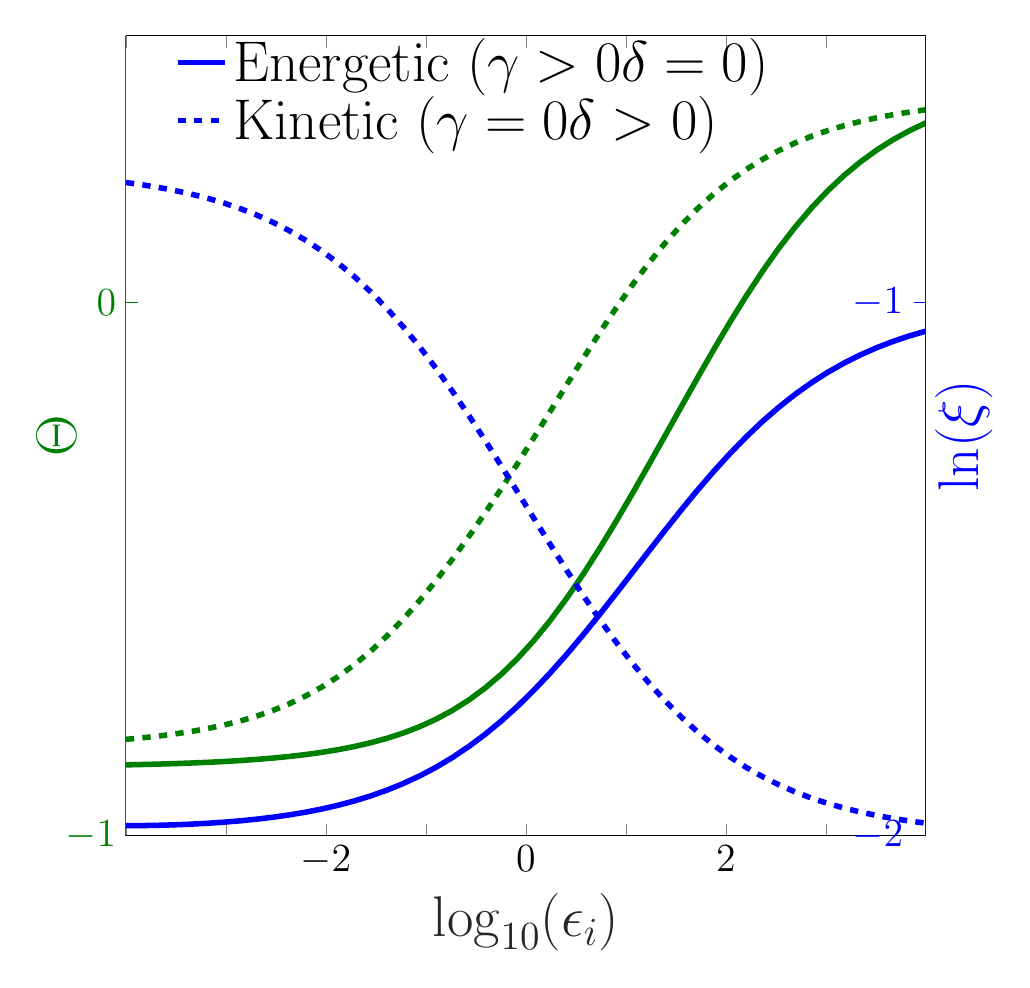
\begin{tikzpicture}

\begin{axis}[%
width=4in,
height=4in,
at={(0in,0in)},
scale only axis,
xmin=-4,
xmax=4,
xtick = {-2,0,2},
xlabel style={font=\huge\color{white!15!black}},
xlabel={$\log_{10}(\epsilon_i)$},
separate axis lines,
axis y line*=left,
every outer y axis line/.append style={black!50!green},
every y tick label/.append style={font=\Large\color{black!50!green}},
every y tick/.append style={black!50!green},
ymin=-1,
ymax=0.5,
ytick={-1, 0},
ylabel style={font=\huge\color{black!50!green}, at={(axis description cs:-0.05,0.5)}},
ylabel={$\Theta$},
axis background/.style={fill=none},
yticklabel pos=right,
]
\addplot [color=black!50!green, line width=2.0pt]
  table[row sep=crcr]{%
-4	-0.86712195063823\\
-3.83673469387755	-0.866459706139752\\
-3.6734693877551	-0.865678189906575\\
-3.51020408163265	-0.86475557792563\\
-3.3469387755102	-0.863665936934352\\
-3.18367346938776	-0.862378416090975\\
-3.02040816326531	-0.86085627230916\\
-2.85714285714286	-0.85905569554162\\
-2.69387755102041	-0.856924395411978\\
-2.53061224489796	-0.854399906776275\\
-2.36734693877551	-0.851407570741511\\
-2.20408163265306	-0.847858152256934\\
-2.04081632653061	-0.843645070263551\\
-1.87755102040816	-0.838641248643482\\
-1.71428571428571	-0.832695656115789\\
-1.55102040816327	-0.82562970449693\\
-1.38775510204082	-0.817233833628389\\
-1.22448979591837	-0.80726484286983\\
-1.06122448979592	-0.795444838492099\\
-0.897959183673469	-0.781463031889889\\
-0.73469387755102	-0.764981970340433\\
-0.571428571428571	-0.745649950371574\\
-0.408163265306122	-0.723121091220409\\
-0.244897959183673	-0.697083503684381\\
-0.0816326530612245	-0.667293932145592\\
0.0816326530612245	-0.633614305190569\\
0.244897959183673	-0.596042655351181\\
0.408163265306122	-0.554729524282433\\
0.571428571428571	-0.509973127376225\\
0.73469387755102	-0.462192880959991\\
0.897959183673469	-0.41188943203243\\
1.06122448979592	-0.359605577480526\\
1.22448979591837	-0.305901913003867\\
1.38775510204082	-0.251352791651361\\
1.55102040816327	-0.196556415902121\\
1.71428571428571	-0.142144604926812\\
1.87755102040816	-0.0887779096369525\\
2.04081632653061	-0.0371198277065357\\
2.20408163265306	0.0122053252255192\\
2.36734693877551	0.0586589016979626\\
2.53061224489796	0.101825813127987\\
2.69387755102041	0.141435331724591\\
2.85714285714286	0.177362780569039\\
3.02040816326531	0.209615375532946\\
3.18367346938776	0.238308104188025\\
3.3469387755102	0.263635665558142\\
3.51020408163265	0.285845149784655\\
3.6734693877551	0.305212329132137\\
3.83673469387755	0.322022821711851\\
4	0.336558248592482\\
};

\addplot [color=black!50!green, dashed, line width=2.0pt]
  table[row sep=crcr]{%
-4	-0.819259085237148\\
-3.83673469387755	-0.816436600053761\\
-3.6734693877551	-0.81310206332122\\
-3.51020408163265	-0.809161928752633\\
-3.3469387755102	-0.804505987746505\\
-3.18367346938776	-0.799004925212739\\
-3.02040816326531	-0.792507905034933\\
-2.85714285714286	-0.784840472540855\\
-2.69387755102041	-0.775803233807122\\
-2.53061224489796	-0.765171991637696\\
-2.36734693877551	-0.752700261698691\\
-2.20408163265306	-0.738125293733678\\
-2.04081632653061	-0.721178752485815\\
-1.87755102040816	-0.701602868600687\\
-1.71428571428571	-0.679171912014443\\
-1.55102040816327	-0.653717117997919\\
-1.38775510204082	-0.625150884190199\\
-1.22448979591837	-0.593483931824915\\
-1.06122448979592	-0.55882862046812\\
-0.897959183673469	-0.521384283325877\\
-0.73469387755102	-0.481406751952637\\
-0.571428571428571	-0.439172189239683\\
-0.408163265306122	-0.394950602920698\\
-0.244897959183673	-0.349002589071998\\
-0.0816326530612245	-0.301603045336879\\
0.0816326530612245	-0.253082089354969\\
0.244897959183673	-0.203863611254387\\
0.408163265306122	-0.154481508535011\\
0.571428571428571	-0.105562941118016\\
0.73469387755102	-0.0577816459859097\\
0.897959183673469	-0.0117953265598192\\
1.06122448979592	0.0318152204206433\\
1.22448979591837	0.0725912351830887\\
1.38775510204082	0.110218876033748\\
1.55102040816327	0.144530624770316\\
1.71428571428571	0.175490575663137\\
1.87755102040816	0.203170442256917\\
2.04081632653061	0.227722367752829\\
2.20408163265306	0.2493528598676\\
2.36734693877551	0.268300310592425\\
2.53061224489796	0.284817080744148\\
2.69387755102041	0.299156155212727\\
2.85714285714286	0.311561844577519\\
3.02040816326531	0.322263794881274\\
3.18367346938776	0.331473546483831\\
3.3469387755102	0.339382961805802\\
3.51020408163265	0.346163959821047\\
3.6734693877551	0.351969117749945\\
3.83673469387755	0.3569328105346\\
4	0.361172649961282\\
};

\end{axis}

\begin{axis}[%
width=4in,
height=4in,
at={(0in,0in)},
scale only axis,
xmin=-4,
xmax=4,
xlabel style={font=\huge\color{white!15!black}},
%xlabel={$\log_{10}(\epsilon_i)$},
xticklabels=\empty,
separate axis lines,
axis y line*=right,
every outer y axis line/.append style={blue},
every y tick label/.append style={font=\Large\color{blue}},
every y tick/.append style={blue},
ymin=-2,
ymax=-0.5,
ytick={-2, -1},
ylabel style={font=\huge\color{blue}},
ylabel={$\ln(\xi)$},
axis background/.style={fill=none},
yticklabel pos=right,
legend style={at={(0.05,0.85)}, anchor=south west, legend cell align=left, align=left, fill=none, draw=none},
y tick label style={xshift={-3em},anchor=west},
]

\addplot [color=blue, line width=2.0pt]
  table[row sep=crcr]{%
-4	-1.98123722630083\\
-3.83673469387755	-1.98098507569647\\
-3.6734693877551	-1.98041596099564\\
-3.51020408163265	-1.97951591044775\\
-3.3469387755102	-1.97826293711223\\
-3.18367346938776	-1.97662665915261\\
-3.02040816326531	-1.97456779767177\\
-2.85714285714286	-1.97203756672901\\
-2.69387755102041	-1.96897697802198\\
-2.53061224489796	-1.96531609352077\\
-2.36734693877551	-1.96097327395976\\
-2.20408163265306	-1.95585448992134\\
-2.04081632653061	-1.94985278596987\\
-1.87755102040816	-1.94284801669057\\
-1.71428571428571	-1.93470700572307\\
-1.55102040816327	-1.92528431282414\\
-1.38775510204082	-1.91442382548764\\
-1.22448979591837	-1.90196141423748\\
-1.06122448979592	-1.88772889507563\\
-0.897959183673469	-1.8715595166127\\
-0.73469387755102	-1.85329511960998\\
-0.571428571428571	-1.83279499011033\\
-0.408163265306122	-1.80994623626516\\
-0.244897959183673	-1.78467526595073\\
-0.0816326530612245	-1.75695964644101\\
0.0816326530612245	-1.72683932838268\\
0.244897959183673	-1.69442597385332\\
0.408163265306122	-1.65990901426636\\
0.571428571428571	-1.62355714622354\\
0.73469387755102	-1.58571429409125\\
0.897959183673469	-1.54678962193927\\
1.06122448979592	-1.50724190030877\\
1.22448979591837	-1.46755930666782\\
1.38775510204082	-1.42823641346829\\
1.55102040816327	-1.38975055232747\\
1.71428571428571	-1.35253984096545\\
1.87755102040816	-1.31698489903049\\
2.04081632653061	-1.2833957181928\\
2.20408163265306	-1.25200441256614\\
2.36734693877551	-1.22296380792583\\
2.53061224489796	-1.1963511712314\\
2.69387755102041	-1.17217593096241\\
2.85714285714286	-1.15039003026085\\
3.02040816326531	-1.13089957007333\\
3.18367346938776	-1.11357658162771\\
3.3469387755102	-1.09827004443767\\
3.51020408163265	-1.08481556977907\\
3.6734693877551	-1.07304344923363\\
3.83673469387755	-1.0627849935446\\
4	-1.05387724783603\\
};
\addlegendentry{Energetic ($\gamma>0\delta=0$)}


\addplot [color=blue, dashed, line width=2.0pt]
  table[row sep=crcr]{%
-4	-0.775217342816201\\
-3.83673469387755	-0.779499644886392\\
-3.6734693877551	-0.78446984017953\\
-3.51020408163265	-0.790239539480914\\
-3.3469387755102	-0.796934171227636\\
-3.18367346938776	-0.804693784190871\\
-3.02040816326531	-0.813673461012692\\
-2.85714285714286	-0.824043159570773\\
-2.69387755102041	-0.835986759864976\\
-2.53061224489796	-0.849700059805028\\
-2.36734693877551	-0.865387442263179\\
-2.20408163265306	-0.883256939452262\\
-2.04081632653061	-0.903513463054251\\
-1.87755102040816	-0.926350064312261\\
-1.71428571428571	-0.95193724975618\\
-1.55102040816327	-0.980410610112542\\
-1.38775510204082	-1.01185731352497\\
-1.22448979591837	-1.0463023418734\\
-1.06122448979592	-1.08369566195231\\
-0.897959183673469	-1.12390175522629\\
-0.73469387755102	-1.16669300822434\\
-0.571428571428571	-1.21174832954486\\
-0.408163265306122	-1.25865798046191\\
-0.244897959183673	-1.3069350043196\\
-0.0816326530612245	-1.35603288870117\\
0.0816326530612245	-1.40536831036891\\
0.244897959183673	-1.45434713244375\\
0.408163265306122	-1.50239137167567\\
0.571428571428571	-1.54896471672523\\
0.73469387755102	-1.59359438245302\\
0.897959183673469	-1.63588759111586\\
1.06122448979592	-1.67554168342151\\
1.22448979591837	-1.71234765050332\\
1.38775510204082	-1.74618760738648\\
1.55102040816327	-1.77702728993695\\
1.71428571428571	-1.80490498754057\\
1.87755102040816	-1.82991841332557\\
2.04081632653061	-1.85221089909396\\
2.20408163265306	-1.8719580480963\\
2.36734693877551	-1.88935565798198\\
2.53061224489796	-1.90460940214291\\
2.69387755102041	-1.91792647484832\\
2.85714285714286	-1.92950918754672\\
3.02040816326531	-1.93955035603465\\
3.18367346938776	-1.94823023414304\\
3.3469387755102	-1.95571471607294\\
3.51020408163265	-1.962154531712\\
3.6734693877551	-1.96768518364264\\
3.83673469387755	-1.97242741029798\\
4	-1.97648799909347\\
};
\addlegendentry{Kinetic ($\gamma=0\delta>0$)}


\end{axis}
\end{tikzpicture}%
}} 
\caption{Orthogonality in the Hopfield-Ninio scheme.  (a) Reaction diagram of the scheme.  Note that in the energetic regime, $k_W$ and $l_W$ will differ from $k_R$ and $l_R$ by a factor $e^{\gamma}$.  In the kinetic regime, $k_R$ and $k^{\prime}_R$ increase by a factor $e^{\delta}$ and $l_W$ and $l^{\prime}_W$ increase by a factor $e^{\delta_p}$ \cite{Rao2015}.  (b) Orthogonality bounds minimum error rate in the energetic regime  ($\gamma=1, \delta=0$). The log of the error rate $(\log(\xi))$ as a function of the orthogonality ($\Theta$) is plotted for simulated data (parameter selection in Methods).   Heatmap coloration represents relative dissipation $\Delta S_i$ \cite{Schnakenberg1976} (hotter is higher dissipation); note that at a given orthogonality level, the error rate decreases as dissipation goes up (more red).  (c) In the energetic  regime, minimum error (red line, $\xi = e^{-2\gamma}$) is achieved by simultaneously minimizing orthogonality ($\Theta$, green) and maximizing dissipation (black).  Excess dissipation drives orthogonality upwards, asymptoting with error equal to the binding energy difference ($\xi = e^{-\gamma}).$   (d) Orthogonality as a function of drive.  In the energetic regime (solid curves), error rate ($\xi$) is minimized in the limit of low orthogonality ($\Theta$). In the kinetic regime, (dashed curves), error rate is minimized in the limit of high orthogonality. \label{fig:hopfield}}
\end{figure*}

Ninio and Hopfield designed this scheme to amplify differences in the binding energies of $EW$ and $ER$ complex formation.  It is instructive to write the rate constants in Kramer's form.

We have for the $EW$ reactions:
\begin{center}
\begin{tabular}{ll}
$k^{\prime}_W = \omega e^\epsilon$ & $l^{\prime}_W = \omega_p$\\
\\
$k_W =  \omega e^\gamma $&$ l_W = \omega_p e^{\epsilon_p+\gamma}$\\
\end{tabular}
\end{center}
where: $\omega, \ \omega_p$ set overall rates; $\epsilon, \epsilon_p$ represent the enthalpy differences between free enzyme and complexes $ES^*, \ ES;$ and $\gamma$ represents the binding energy difference between right and wrong complexes.

The $ER$ reactions are given by:
\begin{center}
\begin{tabular}{ll}
$k^{\prime}_R = \omega e^{\epsilon+\delta}$ & $l^{\prime}_R = \omega_pe^{-\delta_p}$\\
\\
$k_R =  \omega e^\delta $&$ l_R = \omega_p e^{\epsilon_p-\delta_p}$\\
\end{tabular}
\end{center}
where $\delta$ sets the activation energy differences between right and wrong complexes.

There is no discrimination along the transitions between the intermediary and final product:
\begin{center}
\begin{tabular}{ccc}
$m = \omega_i,$  & & $m' = \omega_i e^{\eps_i}$.\\
\\
\end{tabular}
\end{center}

We begin by considering the relationship between error and orthogonality in the regime which is governed only by binding energy differences ($\gamma >0, \ \delta=0$), termed the `energetic regime.'  The Hopfield-Ninio scheme was originally designed for discrimination in this regime: the intermediary complex ($ES^*$) and dissipative drive ($m'$) introduce a delay which amplifies the fact that $EW$ complex formation has a faster off-rate (by factor of $\gamma$) relative to $ER$ formation.  

Simulations reveal that low orthogonality is necessary, but not sufficient, for low error rates in the energetic regime (Figure  \ref{fig:hopfield}(b)).  Analytically, we recall the long appreciated fact that the (energetic) Hopfield-Ninio scheme requires the parametric limit
\[
\frac{\omega_p}{\omega e^{\epsilon}}\rightarrow0 
\]
in order to minimize its error, and demonstrate that orthogonality is monotonically decreasing as this limit is approached (Appendix~\ref{app:hopfield}).

A less well-appreciated requirement for energetic discrimination concerns the nonequilibrium drive, represented by $m'.$  Some amount of drive is crucial for the discrimination scheme to work at all, but too much drive destroys discrimination \cite{Wong2018}.  We can understand this nonlinearity in terms of orthogonality (Figure  \ref{fig:hopfield}(c)).  Energy dissipation~\footnote{Throughout this text dissipation is calculated as the entorpy production rate, \unexpanded{$\Delta S_i = \frac{1}{2}\sum_{i,j}(k_{ij}\rho_j-k_{ji}\rho_i)\ln{\frac{k_{ij}\rho_j}{k_{ji}\rho_i}}$}} is helpful for discrimination up {\it until} the point at which it begins to drive up orthogonality.

We next turn to the regime governed by only activation energy differences ($\gamma =0, \ \delta > 0$), termed the `kinetic regime.'  Simulations reveal a bound opposite to that of the energetic regime: high orthogonality is necessary (but not sufficient) for low error (Supplemental Figure \ref{sfig:kin_sim}).  Analytically, we can derive the error in this regime to be
\[
\xi_{\text{kinetic}} = \frac{1+e^{-\delta}\eta b+e^{-2\delta} \eta c}{1+\eta b+\eta c}
\]
where 
\[
a = \omega\omega_i, \ \ \ b = \omega\omega_p, \ \ \ c = \omega_p\omega_i e^{\epsilon_i}, \ \ \ \eta=e^{\epsilon_p}/a.
\]
The $\xi_{\text{kinetic}}$ is minimized when $\eta\gg1$ and $c\gg b.$  That is, when there exists high drive ($\omega_i e^{\epsilon_i}\gg\omega)$ and free enthalpy product differences ($\epsilon_p\gg0$).  We demonstrate that orthogonality is monotonically {\it increasing} as these limits are approached (Appendix~\ref{app:hopfield}).

Differences between the two discriminatory  regimes are summarized in Figure  \ref{fig:hopfield}(d).  Increasing the dissipative drive ($\eps_i$) increases orthogonality, which allows for kinetic discrimination but precludes energetic discrimination.
\begin{figure}[htbp]
\resizebox{1\columnwidth}{!}{
% This file was created by matlab2tikz.
%
%The latest updates can be retrieved from
%  http://www.mathworks.com/matlabcentral/fileexchange/22022-matlab2tikz-matlab2tikz
%where you can also make suggestions and rate matlab2tikz.
%
\definecolor{mycolor1}{rgb}{0.00000,0.000,0.000}%
%
\begin{tikzpicture}

\begin{axis}[%
%width=4in,
%height=4in,
%at={(0in,0in)},
scale only axis,
axis y line*=left,
xmin=-2,
xmax=8,
xlabel style={font=\huge\bfseries\color{white!15!black}},
xlabel={$\epsilon_i$},
every x tick label/.append style={font=\large},
separate axis lines,
every outer y axis line/.append style={black!50!green},
every y tick label/.append style={font=\large\color{black!50!green}},
every y tick/.append style={black!50!green},
ymin=-0.2,
ymax=0.1,
ytick={-.2, -.1,  0, .1},
ylabel style={font=\huge\bfseries\color{black!50!green}, at={(axis description cs:-0.05,0.5)}},
ylabel={$\Theta$},
axis background/.style={fill=white},
yticklabel pos=right,
legend style={at={(0.4,0.03)}, anchor=south, legend cell align=left, align=left, fill=none, draw=none,font=\Large}
]
\addplot [color=black!50!green, line width=2.0pt, forget plot]
  table[row sep=crcr]{%
-2	-0.145487707741606\\
-1.79591836734694	-0.144361104521461\\
-1.59183673469388	-0.142987721411673\\
-1.38775510204082	-0.141319852985956\\
-1.18367346938776	-0.13930554413684\\
-0.979591836734694	-0.136891944096277\\
-0.775510204081633	-0.134031421425144\\
-0.571428571428571	-0.130691144147433\\
-0.36734693877551	-0.126866035152971\\
-0.163265306122449	-0.122593290923324\\
0.0408163265306123	-0.117964159578255\\
0.244897959183673	-0.113126593679051\\
0.448979591836735	-0.10827293934831\\
0.653061224489796	-0.103611733801414\\
0.857142857142857	-0.0993306059429575\\
1.06122448979592	-0.0955630976762244\\
1.26530612244898	-0.0923709643904862\\
1.46938775510204	-0.0897455940536549\\
1.6734693877551	-0.0876234336915983\\
1.87755102040816	-0.0859062516805647\\
2.08163265306122	-0.0844784680379634\\
2.28571428571429	-0.0832177562900709\\
2.48979591836735	-0.0819986783835916\\
2.69387755102041	-0.0806910990811203\\
2.89795918367347	-0.0791558573892049\\
3.10204081632653	-0.0772404082747666\\
3.30612244897959	-0.0747774030982453\\
3.51020408163265	-0.0715894695365708\\
3.71428571428571	-0.0675032498555324\\
3.91836734693878	-0.0623741121352132\\
4.12244897959184	-0.0561190719829563\\
4.3265306122449	-0.0487498751125661\\
4.53061224489796	-0.0403937284106833\\
4.73469387755102	-0.0312900460142858\\
4.93877551020408	-0.0217597490247694\\
5.14285714285714	-0.012155450998987\\
5.3469387755102	-0.00280876786915538\\
5.55102040816327	0.00600986341632774\\
5.75510204081633	0.0141112298296202\\
5.95918367346939	0.0213883543563436\\
6.16326530612245	0.0278047419198082\\
6.36734693877551	0.0333769712494013\\
6.57142857142857	0.0381569835826827\\
6.77551020408163	0.0422170161993275\\
6.97959183673469	0.0456382074445136\\
7.18367346938776	0.04850275322077\\
7.38775510204082	0.0508889852631445\\
7.59183673469388	0.0528686246014564\\
7.79591836734694	0.0545055382407869\\
8	0.0558554681001441\\
};

\addplot [color=mycolor1, line width=2.0pt]
  table[row sep=crcr]{%
-2	-0.2\\
-1.79591836734694	-0.191132019681701\\
-1.59183673469388	-0.182290885329135\\
-1.38775510204082	-0.173476263514495\\
-1.18367346938776	-0.164688054238085\\
-0.979591836734694	-0.155926403309685\\
-0.775510204081633	-0.147191715979291\\
-0.571428571428571	-0.138484670533798\\
-0.36734693877551	-0.129806230455246\\
-0.163265306122449	-0.121157653916526\\
0.0408163265306123	-0.112540500127849\\
0.244897959183673	-0.103956633638209\\
0.448979591836735	-0.095408230376862\\
0.653061224489796	-0.0868977929850395\\
0.857142857142857	-0.0784281873535753\\
1.06122448979592	-0.0700027161011158\\
1.26530612244898	-0.0616252462523263\\
1.46938775510204	-0.0533004057494227\\
1.6734693877551	-0.0450338555959917\\
1.87755102040816	-0.0368326320608851\\
2.08163265306122	-0.0287055391202966\\
2.28571428571429	-0.0206635589095075\\
2.48979591836735	-0.0127202403370346\\
2.69387755102041	-0.00489202371289099\\
2.89795918367347	0.00280153984669015\\
3.10204081632653	0.0103377145973593\\
3.30612244897959	0.0176906934977098\\
3.51020408163265	0.024831942650711\\
3.71428571428571	0.0317308201473184\\
3.91836734693878	0.0383555025266874\\
4.12244897959184	0.0446742264497309\\
4.3265306122449	0.0506568091846537\\
4.53061224489796	0.0562763526346445\\
4.73469387755102	0.0615109735553188\\
4.93877551020408	0.066345355889387\\
5.14285714285714	0.0707719098453687\\
5.3469387755102	0.0747913593511688\\
5.55102040816327	0.0784126625926542\\
5.75510204081633	0.0816522800654129\\
5.95918367346939	0.08453291067986\\
6.16326530612245	0.0870818901768923\\
6.36734693877551	0.0893294715245012\\
6.57142857142857	0.091307185531165\\
6.77551020408163	0.0930464266584816\\
6.97959183673469	0.0945773440587021\\
7.18367346938776	0.0959280583958961\\
7.38775510204082	0.0971241810673502\\
7.59183673469388	0.0981885867287327\\
7.79591836734694	0.0991413801760296\\
8	0.1\\
};
\addlegendentry{Dissipation (scaled)}
\end{axis}

\begin{axis}[%
scale only axis,
axis y line*=right,
xmin=-2,
xmax=8,
xlabel style={font=\huge\bfseries\color{white!15!black}},
%xlabel={$\log_{10}(\epsilon_i)$},
xtick=\empty,
xticklabels = \empty,
separate axis lines,
every outer y axis line/.append style={blue},
every y tick label/.append style={font=\large\color{blue}},
every y tick/.append style={blue},
ymin=-2,
ymax=2,
ytick={-2, -1,  0,  1,  2},
y tick label style={xshift={-2em},anchor=west},
ylabel style={font=\huge\bfseries\color{blue}},
ylabel={$\ln(\rho_\gamma/\rho_\delta)$},
axis background/.style={fill=none},
yticklabel pos=right,
y tick label style={xshift={-1.5em},anchor=west},
legend style={at={(0.5,0.03)}, anchor=south, legend cell align=left, align=left, fill=none, draw=none}
]


\addplot [color=blue, line width=2.0pt, forget plot]
  table[row sep=crcr]{%
-2	1.88660938038003\\
-1.79591836734694	1.87435017907208\\
-1.59183673469388	1.85785211898435\\
-1.38775510204082	1.83665508146175\\
-1.18367346938776	1.81021201331722\\
-0.979591836734694	1.77790107059703\\
-0.775510204081633	1.7390448709167\\
-0.571428571428571	1.69293785127123\\
-0.36734693877551	1.63888192177135\\
-0.163265306122449	1.57622932373893\\
0.0408163265306123	1.50442999225127\\
0.244897959183673	1.42307913394178\\
0.448979591836735	1.33195965646555\\
0.653061224489796	1.23107401760636\\
0.857142857142857	1.12066125972224\\
1.06122448979592	1.00119730476016\\
1.26530612244898	0.873379424552053\\
1.46938775510204	0.738098364564633\\
1.6734693877551	0.596403182803249\\
1.87755102040816	0.449464136570183\\
2.08163265306122	0.298538020879727\\
2.28571428571429	0.144938664088435\\
2.48979591836735	-0.00998665259225849\\
2.69387755102041	-0.164875820935063\\
2.89795918367347	-0.318367799007411\\
3.10204081632653	-0.46911863101273\\
3.30612244897959	-0.615820429883564\\
3.51020408163265	-0.757225477587848\\
3.71428571428571	-0.892176306779867\\
3.91836734693878	-1.0196408676989\\
4.12244897959184	-1.13874994812297\\
4.3265306122449	-1.24883235538962\\
4.53061224489796	-1.34944251680539\\
4.73469387755102	-1.44037552308464\\
4.93877551020408	-1.52166631195306\\
5.14285714285714	-1.59357230145826\\
5.3469387755102	-1.65654161285406\\
5.55102040816327	-1.71117127049288\\
5.75510204081633	-1.7581608745756\\
5.95918367346939	-1.79826708910277\\
6.16326530612245	-1.83226315457867\\
6.36734693877551	-1.8609060194387\\
6.57142857142857	-1.88491207199282\\
6.77551020408163	-1.90494117372672\\
6.97959183673469	-1.92158787629055\\
7.18367346938776	-1.93537832504212\\
7.38775510204082	-1.94677130516029\\
7.59183673469388	-1.95616204535988\\
7.79591836734694	-1.9638876501685\\
8	-1.9702333080646\\
};
\addplot [color=red, dashed, forget plot]
  table[row sep=crcr]{%
-2	0\\
8	0\\
};
\end{axis}

\end{tikzpicture}% }
\caption{A Hopfield-Ninio style network designed to tune product selectivity by modulating dissipation (black).  One product $\rho_{\gamma}$ has a lower binding energy and is favored in the energetic regime, while the other $\rho_{\delta}$ is has a lower activation energy and is favored in the kinetic regime.  The log of the ratio between the products ($\rho_{\gamma}$/$\rho_{\delta}$, blue), can be shifted from 2 ($\rho_{\gamma}$  favored) to -2 ($\rho_{\delta}$ favored) by driving across a single reaction.  This is due to orthogonality (green line) increasing, which shifts the network from the energetic to the kinetic regime. \label{fig:hop_switch}}

\end{figure}


The ability to modulate orthogonality via driving the single reaction $m'$ suggests a simple strategy for dissipation-driven product switching.
If products $EW, \ ER$ are favored by different energy types, they can be selected between only by driving $m'$ such that the network moves from low to high orthogonality. We achieve a four order of magnitude selection effect via this scheme (Figure~\ref{fig:hop_switch}).

Because the Hopfield-Ninio scheme only has one intermediary product, it is difficult to interpret in terms of the number of effective pathways towards the discriminatory products.  In order to illustrate the connection between discrimination, effective pathways, and orthogonality, we turn to a more general setting.
\section{Orthogonality in a general setting}
\begin{figure*}[ht]
\subfigure[]{
 \resizebox{0.4\textwidth}{!}{
\scalebox{.4}{
\schemestart
0 \arrow(0--$y_{s0}$){<=>[$\mathrm{k_{on}}$][$\mathrm{k_{off}}$]}[,,,red] $y_{s0}$
\arrow{<=>[$u^S$][$d^S$]}[90,,,red] 
$x_{s0}$ \arrow($x_{s0}$--$x_{s1}$){->[$f$]}[,,,red]$x_{s1}$
\arrow(@$y_{s0}$--$y_{s1}$){<-[][$b$]}[,,,red] $y_{s1}$ \arrow{<=>[$u^S$][$d^S$]}[90,,,red]
\arrow(@$y_{s1}$--$y_{s2}$){<-[][$b$]}[,,,red] $y_{s2}$
\arrow{<=>[$u^S$][$d^S$]}[90,,,red] 
\arrow(@$x_{s1}$--$x_{s2}$){->[$f$]}[,,,red] $x_{s2}$
\schemestop}
}} 
\subfigure[]{
\resizebox{0.4\textwidth}{!}{
% This file was created by matlab2tikz.
%
%The latest updates can be retrieved from
%  http://www.mathworks.com/matlabcentral/fileexchange/22022-matlab2tikz-matlab2tikz
%where you can also make suggestions and rate matlab2tikz.
%
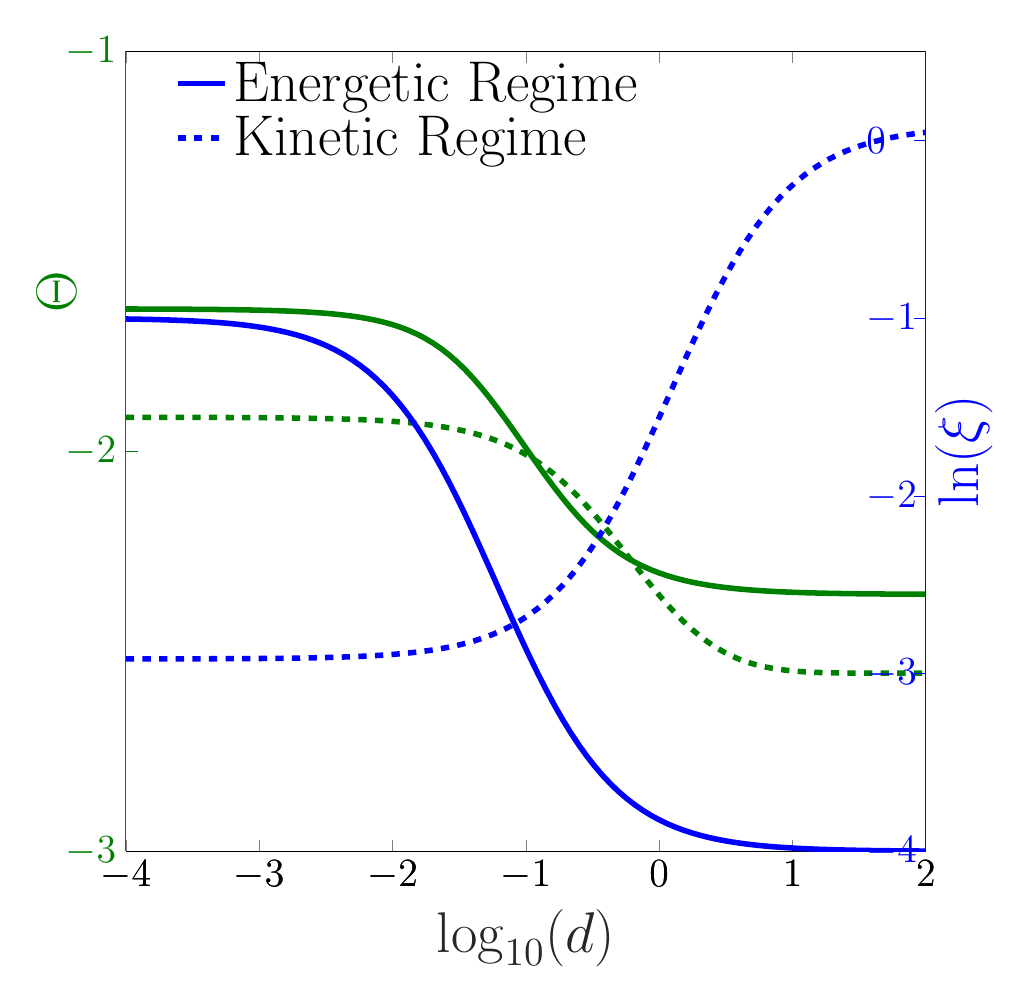
\begin{tikzpicture}


\begin{axis}[%
width=4in,
height=4in,
at={(0in,0in)},
scale only axis,
xmin=-4,
xmax=2,
xlabel style={font=\huge\color{white!15!black}},
xlabel={$\log_{10}(d)$},
separate axis lines,
axis y line*=left,
every outer y axis line/.append style={black!50!green},
every y tick label/.append style={font=\Large\color{black!50!green}},
every y tick/.append style={black!50!green},
ymin=-3,
ymax=-1,
ytick={-3, -2, -1},
ylabel style={font=\huge\color{black!50!green}, at={(axis description cs:-0.05,0.7)}},
ylabel={$\Theta$},
axis background/.style={fill=none},
yticklabel pos=right,
]

\addplot [color=black!50!green, line width=2.0pt]
  table[row sep=crcr]{%
-4	-1.64399326616915\\
-3.93939393939394	-1.64404192835098\\
-3.87878787878788	-1.64409793618038\\
-3.81818181818182	-1.64416240826328\\
-3.75757575757576	-1.6442366366041\\
-3.6969696969697	-1.64432211441953\\
-3.63636363636364	-1.64442056868828\\
-3.57575757575758	-1.64453399831721\\
-3.51515151515152	-1.64466471898601\\
-3.45454545454545	-1.64481541595269\\
-3.39393939393939	-1.64498920637236\\
-3.33333333333333	-1.64518971300906\\
-3.27272727272727	-1.64542115161907\\
-3.21212121212121	-1.64568843476475\\
-3.15151515151515	-1.64599729539496\\
-3.09090909090909	-1.64635443421425\\
-3.03030303030303	-1.64676769566845\\
-2.96969696969697	-1.64724627830413\\
-2.90909090909091	-1.64780098630998\\
-2.84848484848485	-1.64844453019668\\
-2.78787878787879	-1.64919188577388\\
-2.72727272727273	-1.65006072175416\\
-2.66666666666667	-1.65107190731864\\
-2.60606060606061	-1.65225011161501\\
-2.54545454545455	-1.6536245071292\\
-2.48484848484848	-1.65522958777301\\
-2.42424242424242	-1.65710610980957\\
-2.36363636363636	-1.65930215865735\\
-2.3030303030303	-1.66187433614615\\
-2.24242424242424	-1.66488904945341\\
-2.18181818181818	-1.66842386241833\\
-2.12121212121212	-1.67256883854191\\
-2.06060606060606	-1.67742775702973\\
-2	-1.68311901075324\\
-1.93939393939394	-1.68977588930481\\
-1.87878787878788	-1.69754580781161\\
-1.81818181818182	-1.70658787733804\\
-1.75757575757576	-1.71706807838909\\
-1.6969696969697	-1.72915130506177\\
-1.63636363636364	-1.74298985336353\\
-1.57575757575758	-1.75870867512171\\
-1.51515151515152	-1.77638889315987\\
-1.45454545454545	-1.79605234958365\\
-1.39393939393939	-1.8176506943523\\
-1.33333333333333	-1.84106203380798\\
-1.27272727272727	-1.86609623609104\\
-1.21212121212121	-1.8925072698768\\
-1.15151515151515	-1.92000875215079\\
-1.09090909090909	-1.94828843522621\\
-1.03030303030303	-1.97701897326746\\
-0.96969696969697	-2.00586505820671\\
-0.909090909090909	-2.0344893131226\\
-0.848484848484849	-2.06255991008871\\
-0.787878787878788	-2.08976156016614\\
-0.727272727272727	-2.11580923915707\\
-0.666666666666667	-2.14046212308555\\
-0.606060606060606	-2.1635346348534\\
-0.545454545454545	-2.18490230024756\\
-0.484848484848485	-2.20450164703108\\
-0.424242424242424	-2.22232486634054\\
-0.363636363636364	-2.23841087687506\\
-0.303030303030303	-2.25283467732429\\
-0.242424242424242	-2.26569661256779\\
-0.181818181818182	-2.27711267826629\\
-0.121212121212121	-2.2872064658982\\
-0.0606060606060606	-2.2961029304659\\
0	-2.30392388545994\\
0.0606060606060605	-2.31078498148072\\
0.121212121212121	-2.31679387197855\\
0.181818181818182	-2.32204927589366\\
0.242424242424242	-2.32664068379999\\
0.303030303030303	-2.33064850205503\\
0.363636363636363	-2.33414447707813\\
0.424242424242424	-2.33719228365249\\
0.484848484848484	-2.33984819512561\\
0.545454545454546	-2.34216177962075\\
0.606060606060606	-2.34417658584804\\
0.666666666666667	-2.34593079609861\\
0.727272727272728	-2.34745783377239\\
0.787878787878788	-2.34878691941395\\
0.848484848484849	-2.34994357358098\\
0.909090909090909	-2.35095006761689\\
0.96969696969697	-2.35182582503789\\
1.03030303030303	-2.35258777713554\\
1.09090909090909	-2.35325067679274\\
1.15151515151515	-2.35382737459139\\
1.21212121212121	-2.35432906117542\\
1.27272727272727	-2.35476547960479\\
1.33333333333333	-2.35514511114961\\
1.39393939393939	-2.35547533766224\\
1.45454545454545	-2.35576258335295\\
1.51515151515152	-2.35601243849333\\
1.57575757575758	-2.35622976728937\\
1.63636363636364	-2.35641880190706\\
1.6969696969697	-2.35658322439742\\
1.75757575757576	-2.35672623805702\\
1.81818181818182	-2.35685062957085\\
1.87878787878788	-2.35695882311754\\
1.93939393939394	-2.35705292746852\\
2	-2.35713477698292\\
};

\addplot [color=black!50!green, dashed, line width=2.0pt]
  table[row sep=crcr]{%
-4	-1.91481446824113\\
-3.93939393939394	-1.9148298348327\\
-3.87878787878788	-1.91484750214673\\
-3.81818181818182	-1.91486781456116\\
-3.75757575757576	-1.9148911679718\\
-3.6969696969697	-1.91491801748972\\
-3.63636363636364	-1.91494888628565\\
-3.57575757575758	-1.91498437575135\\
-3.51515151515152	-1.91502517717279\\
-3.45454545454545	-1.9150720851381\\
-3.39393939393939	-1.91512601293614\\
-3.33333333333333	-1.915188010238\\
-3.27272727272727	-1.91525928339577\\
-3.21212121212121	-1.91534121874103\\
-3.15151515151515	-1.91543540931892\\
-3.09090909090909	-1.91554368555538\\
-3.03030303030303	-1.91566815042374\\
-2.96969696969697	-1.91581121975437\\
-2.90909090909091	-1.91597566841799\\
-2.84848484848485	-1.91616468320962\\
-2.78787878787879	-1.91638192336725\\
-2.72727272727273	-1.91663158977664\\
-2.66666666666667	-1.91691850404158\\
-2.60606060606061	-1.91724819873643\\
-2.54545454545455	-1.91762702030312\\
-2.48484848484848	-1.91806224620511\\
-2.42424242424242	-1.9185622181021\\
-2.36363636363636	-1.91913649295328\\
-2.3030303030303	-1.91979601408463\\
-2.24242424242424	-1.92055330435133\\
-2.18181818181818	-1.92142268356949\\
-2.12121212121212	-1.92242051235236\\
-2.06060606060606	-1.9235654643254\\
-2	-1.92487882835762\\
-1.93939393939394	-1.92638484185953\\
-1.87878787878788	-1.92811105526463\\
-1.81818181818182	-1.93008872640228\\
-1.75757575757576	-1.93235324141957\\
-1.6969696969697	-1.93494455600534\\
-1.63636363636364	-1.93790764664566\\
-1.57575757575758	-1.94129295617461\\
-1.51515151515152	-1.94515681060063\\
-1.45454545454545	-1.94956177467814\\
-1.39393939393939	-1.95457690155718\\
-1.33333333333333	-1.96027781678382\\
-1.27272727272727	-1.96674655890967\\
-1.21212121212121	-1.97407107849447\\
-1.15151515151515	-1.98234427578118\\
-1.09090909090909	-1.99166243770874\\
-1.03030303030303	-2.00212292231591\\
-0.96969696969697	-2.01382094097902\\
-0.909090909090909	-2.02684531758016\\
-0.848484848484849	-2.0412731725577\\
-0.787878787878788	-2.0571636029392\\
-0.727272727272727	-2.07455061550642\\
-0.666666666666667	-2.09343581287762\\
-0.606060606060606	-2.1137815982259\\
-0.545454545454545	-2.13550588368954\\
-0.484848484848485	-2.15847935675654\\
-0.424242424242424	-2.18252616925136\\
-0.363636363636364	-2.20742841036492\\
-0.303030303030303	-2.2329339806899\\
-0.242424242424242	-2.25876673347223\\
-0.181818181818182	-2.28463732632825\\
-0.121212121212121	-2.31025338587006\\
-0.0606060606060606	-2.3353283002312\\
0	-2.35958884925627\\
0.0606060606060605	-2.38278243596321\\
0.121212121212121	-2.40468456319652\\
0.181818181818182	-2.4251065017565\\
0.242424242424242	-2.44390228323638\\
0.303030303030303	-2.46097373689577\\
0.363636363636363	-2.47627250982277\\
0.424242424242424	-2.48979869935911\\
0.484848484848484	-2.50159647984848\\
0.545454545454546	-2.51174756838448\\
0.606060606060606	-2.5203634512702\\
0.666666666666667	-2.52757712965795\\
0.727272727272728	-2.53353494628937\\
0.787878787878788	-2.53838893437811\\
0.848484848484849	-2.54229006820927\\
0.909090909090909	-2.54538272584727\\
0.96969696969697	-2.54780055756955\\
1.03030303030303	-2.54966380027753\\
1.09090909090909	-2.55107792783941\\
1.15151515151515	-2.55213341662683\\
1.21212121212121	-2.55290635063319\\
1.27272727272727	-2.5534595874259\\
1.33333333333333	-2.55384423921235\\
1.39393939393939	-2.55410127462338\\
1.45454545454545	-2.55426310194179\\
1.51515151515152	-2.55435504423941\\
1.57575757575758	-2.55439665689\\
1.63636363636364	-2.5544028672841\\
1.6969696969697	-2.554384936331\\
1.75757575757576	-2.55435125337981\\
1.81818181818182	-2.55430798254559\\
1.87878787878788	-2.55425958087953\\
1.93939393939394	-2.55420920879764\\
2	-2.55415905172779\\
};

\end{axis}

\begin{axis}[%
width=4in,
height=4in,
at={(0in,0in)},
scale only axis,
xmin=-4,
xmax=2,
xlabel style={font=\huge\color{white!15!black}},
%xlabel={$\log(d)$},
separate axis lines,
axis y line*=right,
every outer y axis line/.append style={blue},
every y tick label/.append style={font=\Large\color{blue}},
every y tick/.append style={blue},
ymin=-4,
ymax=0.5,
ytick={-4, -3, -2, -1, 0},
ylabel style={font=\huge\color{blue}},
ylabel={$\ln(\xi)$},
y tick label style={xshift={-2.5em},anchor=west},
axis background/.style={fill=none},
yticklabel pos=right,
legend style={at={(0.05,0.85)}, anchor=south west, legend cell align=left, align=left, fill=none, draw=none}
]
\addplot [color=blue, line width=2.0pt]
  table[row sep=crcr]{%
-4	-1.00514528094671\\
-3.93939393939394	-1.00591417966106\\
-3.87878787878788	-1.00679769874349\\
-3.81818181818182	-1.00781283426098\\
-3.75757575757576	-1.00897907348236\\
-3.6969696969697	-1.01031875073412\\
-3.63636363636364	-1.01185745110524\\
-3.57575757575758	-1.01362446746407\\
-3.51515151515152	-1.01565331654621\\
-3.45454545454545	-1.01798232005898\\
-3.39393939393939	-1.02065525676499\\
-3.33333333333333	-1.0237220912662\\
-3.27272727272727	-1.02723978462868\\
-3.21212121212121	-1.03127319090066\\
-3.15151515151515	-1.03589604184445\\
-3.09090909090909	-1.04119201958538\\
-3.03030303030303	-1.04725591313774\\
-2.96969696969697	-1.05419484957228\\
-2.90909090909091	-1.06212958358863\\
-2.84848484848485	-1.07119582004068\\
-2.78787878787879	-1.08154553210583\\
-2.72727272727273	-1.09334822287825\\
-2.66666666666667	-1.10679205985796\\
-2.60606060606061	-1.12208478993182\\
-2.54545454545455	-1.13945431712213\\
-2.48484848484848	-1.15914879722334\\
-2.42424242424242	-1.18143607377528\\
-2.36363636363636	-1.20660225092131\\
-2.3030303030303	-1.23494917412145\\
-2.24242424242424	-1.26679057444976\\
-2.18181818181818	-1.30244663289609\\
-2.12121212121212	-1.34223674568556\\
-2.06060606060606	-1.38647032888462\\
-2	-1.43543559883289\\
-1.93939393939394	-1.48938641030531\\
-1.87878787878788	-1.54852742808911\\
-1.81818181818182	-1.61299814355508\\
-1.75757575757576	-1.68285650931167\\
-1.6969696969697	-1.75806322401915\\
-1.63636363636364	-1.83846791692171\\
-1.57575757575758	-1.9237986117283\\
-1.51515151515152	-2.01365584664532\\
-1.45454545454545	-2.10751265658967\\
-1.39393939393939	-2.20472127100837\\
-1.33333333333333	-2.30452686214559\\
-1.27272727272727	-2.4060880428896\\
-1.21212121212121	-2.50850313827492\\
-1.15151515151515	-2.61084063524474\\
-1.09090909090909	-2.71217174610758\\
-1.03030303030303	-2.81160277769924\\
-0.96969696969697	-2.90830502080043\\
-0.909090909090909	-3.00154015910906\\
-0.848484848484849	-3.09067969712817\\
-0.787878787878788	-3.17521754181492\\
-0.727272727272727	-3.25477554766662\\
-0.666666666666667	-3.32910245591022\\
-0.606060606060606	-3.39806715201836\\
-0.545454545454545	-3.46164748844058\\
-0.484848484848485	-3.51991606070038\\
-0.424242424242424	-3.57302430296156\\
-0.363636363636364	-3.62118612131327\\
-0.303030303030303	-3.66466205561363\\
-0.242424242424242	-3.70374469886533\\
-0.181818181818182	-3.73874584424297\\
-0.121212121212121	-3.76998560008697\\
-0.0606060606060606	-3.79778352731955\\
0	-3.82245171631547\\
0.0606060606060605	-3.84428962941829\\
0.121212121212121	-3.86358048405467\\
0.181818181818182	-3.88058893117624\\
0.242424242424242	-3.89555978658208\\
0.303030303030303	-3.90871758951584\\
0.363636363636363	-3.92026678876241\\
0.424242424242424	-3.93039238562434\\
0.484848484848484	-3.93926089283758\\
0.545454545454546	-3.9470214959465\\
0.606060606060606	-3.95380732814733\\
0.666666666666667	-3.959736792711\\
0.727272727272728	-3.96491488266595\\
0.787878787878788	-3.96943446101102\\
0.848484848484849	-3.973377483421\\
0.909090909090909	-3.97681613357599\\
0.96969696969697	-3.97981389066919\\
1.03030303030303	-3.98242651060806\\
1.09090909090909	-3.9847028629193\\
1.15151515151515	-3.98668577994793\\
1.21212121212121	-3.98841269880268\\
1.27272727272727	-3.98991648551135\\
1.33333333333333	-3.99122571565551\\
1.39393939393939	-3.99236533651757\\
1.45454545454545	-3.99335723249601\\
1.51515151515152	-3.99422049656245\\
1.57575757575758	-3.99497302431736\\
1.63636363636364	-3.99562730771617\\
1.6969696969697	-3.99619844791424\\
1.75757575757576	-3.99668129038028\\
1.81818181818182	-3.99712192780194\\
1.87878787878788	-3.99748647550716\\
1.93939393939394	-3.99786080870592\\
2	-3.99808968513925\\
};
\addlegendentry{Energetic Regime}

\addplot [color=blue, dashed, line width=2.0pt]
  table[row sep=crcr]{%
-4	-2.91733526286331\\
-3.93939393939394	-2.91729665488815\\
-3.87878787878788	-2.9172523331581\\
-3.81818181818182	-2.91720127268045\\
-3.75757575757576	-2.91714268818111\\
-3.6969696969697	-2.9170752463596\\
-3.63636363636364	-2.91699769207382\\
-3.57575757575758	-2.91690860022524\\
-3.51515151515152	-2.91680611008076\\
-3.45454545454545	-2.9166882797432\\
-3.39393939393939	-2.91655286015101\\
-3.33333333333333	-2.91639716700639\\
-3.27272727272727	-2.9162182235781\\
-3.21212121212121	-2.91601240550786\\
-3.15151515151515	-2.91577587944173\\
-3.09090909090909	-2.91550394190394\\
-3.03030303030303	-2.91519134182915\\
-2.96969696969697	-2.91483206628571\\
-2.90909090909091	-2.91441904590452\\
-2.84848484848485	-2.91394435382346\\
-2.78787878787879	-2.91339880870926\\
-2.72727272727273	-2.91277178955527\\
-2.66666666666667	-2.91205120524763\\
-2.60606060606061	-2.9112232006956\\
-2.54545454545455	-2.91027178413835\\
-2.48484848484848	-2.90917870141141\\
-2.42424242424242	-2.90792299308768\\
-2.36363636363636	-2.90648064348341\\
-2.3030303030303	-2.90482416309134\\
-2.24242424242424	-2.90292205389708\\
-2.18181818181818	-2.90073833735418\\
-2.12121212121212	-2.8982317585911\\
-2.06060606060606	-2.89535555974875\\
-2	-2.89205598242962\\
-1.93939393939394	-2.88827202718007\\
-1.87878787878788	-2.88393422752991\\
-1.81818181818182	-2.87896370481408\\
-1.75757575757576	-2.87327099099649\\
-1.6969696969697	-2.86675483431648\\
-1.63636363636364	-2.85930108985984\\
-1.57575757575758	-2.85078116591016\\
-1.51515151515152	-2.84105079330144\\
-1.45454545454545	-2.82994894009253\\
-1.39393939393939	-2.81729614981449\\
-1.33333333333333	-2.80289394873099\\
-1.27272727272727	-2.78652393901491\\
-1.21212121212121	-2.76794736456465\\
-1.15151515151515	-2.74690544553906\\
-1.09090909090909	-2.72312038052378\\
-1.03030303030303	-2.69629725719873\\
-0.96969696969697	-2.66612738985531\\
-0.909090909090909	-2.63229274569193\\
-0.848484848484849	-2.59447256036931\\
-0.787878787878788	-2.55235151278722\\
-0.727272727272727	-2.50562991252936\\
-0.666666666666667	-2.45403615697698\\
-0.606060606060606	-2.39734065674789\\
-0.545454545454545	-2.33537144498335\\
-0.484848484848485	-2.26803045132387\\
-0.424242424242424	-2.1953097212927\\
-0.363636363636364	-2.11730621909417\\
-0.303030303030303	-2.03423405260551\\
-0.242424242424242	-1.94643279032296\\
-0.181818181818182	-1.85437025025582\\
-0.121212121212121	-1.75863908276304\\
-0.0606060606060606	-1.65994626600367\\
0	-1.5590957150624\\
0.0606060606060605	-1.45696453421263\\
0.121212121212121	-1.35447427042031\\
0.181818181818182	-1.25255908536176\\
0.242424242424242	-1.15213298185254\\
0.303030303030303	-1.05405849188407\\
0.363636363636363	-0.959118954912089\\
0.424242424242424	-0.867996147764197\\
0.484848484848484	-0.781254438812565\\
0.545454545454546	-0.699331977944571\\
0.606060606060606	-0.622538760488771\\
0.666666666666667	-0.551060854058421\\
0.727272727272728	-0.484969675914825\\
0.787878787878788	-0.424234967497944\\
0.848484848484849	-0.368740076698282\\
0.909090909090909	-0.318298248440627\\
0.96969696969697	-0.27266881545735\\
1.03030303030303	-0.231572440573928\\
1.09090909090909	-0.194704819396904\\
1.15151515151515	-0.161748501216313\\
1.21212121212121	-0.132382693033455\\
1.27272727272727	-0.106291071286463\\
1.33333333333333	-0.0831677381019672\\
1.39393939393939	-0.062721527787329\\
1.45454545454545	-0.0446789024768589\\
1.51515151515152	-0.0287856831583516\\
1.57575757575758	-0.0148078508395435\\
1.63636363636364	-0.00253163043221874\\
1.6969696969697	0.00823695821086093\\
1.75757575757576	0.0176729273441505\\
1.81818181818182	0.0259334005293425\\
1.87878787878788	0.0331588443184213\\
1.93939393939394	0.0394743756237139\\
2	0.0449910875055136\\
};
\addlegendentry{Kinetic Regime}
\end{axis}

\end{tikzpicture}%
}} 
\subfigure[]{
 \resizebox{0.4\textwidth}{!}{
% This file was created by matlab2tikz.
%
%The latest updates can be retrieved from
%  http://www.mathworks.com/matlabcentral/fileexchange/22022-matlab2tikz-matlab2tikz
%where you can also make suggestions and rate matlab2tikz.
%
\definecolor{mycolor1}{rgb}{0.00000,0.000,0.000}%
%
\begin{tikzpicture}

\begin{axis}[%
width=4in,
height=4in,
at={(0in,0in)},
scale only axis,
xmin=-5,
xmax=5,
xtick={-4,-2,0,2,4},
xlabel style={font=\huge\color{white!15!black}},
xlabel={$\log_{10}(\omega_f)$},
separate axis lines,
axis y line*=left,
every outer y axis line/.append style={black!50!green},
every y tick label/.append style={font=\Large\color{black!50!green}},
every y tick/.append style={black!50!green},
ymin=-2.75,
ymax=-1.5,
ytick={-2.5, -2, -1.5},
ylabel style={font=\huge\color{black!50!green}, at={(axis description cs:-0.05,0.5)}},
ylabel={$\Theta$},
axis background/.style={fill=white},
yticklabel pos=right,
]
\addplot [color=black!50!green, line width=2.0pt, forget plot]
  table[row sep=crcr]{%
-5	-2.55980435421901\\
-4.79591836734694	-2.55980434186469\\
-4.59183673469388	-2.55980432209932\\
-4.38775510204082	-2.55980429047699\\
-4.18367346938776	-2.55980423988437\\
-3.97959183673469	-2.55980415893989\\
-3.77551020408163	-2.55980402943132\\
-3.57142857142857	-2.55980382221328\\
-3.36734693877551	-2.55980349063582\\
-3.16326530612245	-2.55980296001059\\
-2.95918367346939	-2.55980211070605\\
-2.75510204081633	-2.55980075096846\\
-2.55102040816327	-2.55979857309744\\
-2.3469387755102	-2.55979508245834\\
-2.14285714285714	-2.55978948167668\\
-1.93877551020408	-2.55978047965553\\
-1.73469387755102	-2.55976597146412\\
-1.53061224489796	-2.55974248912179\\
-1.3265306122449	-2.55970422882944\\
-1.12244897959184	-2.55964125714501\\
-0.918367346938776	-2.55953604663673\\
-0.714285714285714	-2.55935646634765\\
-0.510204081632653	-2.55904103103071\\
-0.306122448979592	-2.55846711374081\\
-0.102040816326531	-2.5573824631785\\
0.102040816326531	-2.55526283181266\\
0.306122448979592	-2.55104223244863\\
0.510204081632653	-2.54269657640861\\
0.714285714285714	-2.52686849980221\\
0.918367346938776	-2.49912348695541\\
1.12244897959184	-2.45540097667699\\
1.3265306122449	-2.39424027330782\\
1.53061224489796	-2.31872009496065\\
1.73469387755102	-2.23643351774748\\
1.93877551020408	-2.15689809777501\\
2.14285714285714	-2.08834622985733\\
2.3469387755102	-2.03500453117392\\
2.55102040816327	-1.99664670020636\\
2.75510204081633	-1.97050192502729\\
2.95918367346939	-1.95327271307917\\
3.16326530612245	-1.94215019118093\\
3.36734693877551	-1.93505897490393\\
3.57142857142857	-1.93057213060324\\
3.77551020408163	-1.92774632352692\\
3.97959183673469	-1.92597172389132\\
4.18367346938776	-1.92485925344566\\
4.38775510204082	-1.92416262937327\\
4.59183673469388	-1.92372670529494\\
4.79591836734694	-1.92345403508248\\
5	-1.92328352551524\\
};
\end{axis}

\begin{axis}[%
width=4in,
height=4in,
at={(0in,0in)},
scale only axis,
xmin=-5,
xmax=5,
xticklabels=\empty,
xlabel style={font=\huge\color{white!15!black}},
%xlabel={$\log(\omega_u)$},
separate axis lines,
axis y line*=right,
every outer y axis line/.append style={mycolor1},
every y tick label/.append style={font=\Large\color{mycolor1}},
every y tick/.append style={mycolor1},
ymin=-4,
ymax=-1,
ytick={-4, -3, -2, -1},
ylabel style={font=\huge\color{mycolor1}},
ylabel={$\log_{10}(\Delta S_i)$},
axis background/.style={fill=none},
yticklabel pos=right,
y tick label style={xshift={-3em},anchor=west},
legend style={at={(0.6,0.05)}, anchor=south west, legend cell align=left, align=left, fill=none, draw=none}
]

\addplot [color=blue, line width=2.0pt, forget plot]
  table[row sep=crcr]{%
-5	-1.00324296746153\\
-4.79591836734694	-1.00518467413702\\
-4.59183673469388	-1.00828549615505\\
-4.38775510204082	-1.01323202156867\\
-4.18367346938776	-1.02110924875673\\
-3.97959183673469	-1.03361913372891\\
-3.77551020408163	-1.05339987998379\\
-3.57142857142857	-1.08446353259473\\
-3.36734693877551	-1.13272573962688\\
-3.16326530612245	-1.20647977484271\\
-2.95918367346939	-1.31641151433184\\
-2.75510204081633	-1.47437574670688\\
-2.55102040816327	-1.68995928856333\\
-2.3469387755102	-1.96465461174935\\
-2.14285714285714	-2.28595937068162\\
-1.93877551020408	-2.62636142678962\\
-1.73469387755102	-2.95063990095384\\
-1.53061224489796	-3.22806606517476\\
-1.3265306122449	-3.44111528773649\\
-1.12244897959184	-3.58576962009024\\
-0.918367346938776	-3.66577229798171\\
-0.714285714285714	-3.68607304168395\\
-0.510204081632653	-3.64871549658509\\
-0.306122448979592	-3.55192606283928\\
-0.102040816326531	-3.39221649509467\\
0.102040816326531	-3.16896104158826\\
0.306122448979592	-2.88979991881088\\
0.510204081632653	-2.57367134356986\\
0.714285714285714	-2.24849026618408\\
0.918367346938776	-1.94372872033049\\
1.12244897959184	-1.68194322093462\\
1.3265306122449	-1.47391420758324\\
1.53061224489796	-1.31912683924617\\
1.73469387755102	-1.20982856438329\\
1.93877551020408	-1.13562465336114\\
2.14285714285714	-1.08663874885576\\
2.3469387755102	-1.05491500175665\\
2.55102040816327	-1.03463054724113\\
2.75510204081633	-1.02176752688542\\
2.95918367346939	-1.01365391259384\\
3.16326530612245	-1.00855333369983\\
3.36734693877551	-1.00535371204537\\
3.57142857142857	-1.00334927787622\\
3.77551020408163	-1.00209461395054\\
3.97959183673469	-1.00130969368936\\
4.18367346938776	-1.00081879269932\\
4.38775510204082	-1.00051189105748\\
4.59183673469388	-1.00031998008897\\
4.79591836734694	-1.00019988932097\\
5	-1.00012504294194\\
};

\addplot [color=mycolor1, line width=2.0pt]
  table[row sep=crcr]{%
-5	-10.4887860431965\\
-4.79591836734694	-10.018872539903\\
-4.59183673469388	-9.54896013053914\\
-4.38775510204082	-9.07904947305567\\
-4.18367346938776	-8.60914162277903\\
-3.97959183673469	-8.13923827509998\\
-3.77551020408163	-7.66934216049719\\
-3.57142857142857	-7.19945769439776\\
-3.36734693877551	-6.72959206421324\\
-3.16326530612245	-6.2597570963748\\
-2.95918367346939	-5.78997259808786\\
-2.75510204081633	-5.32027272040396\\
-2.55102040816327	-4.85071916882426\\
-2.3469387755102	-4.38143173349484\\
-2.14285714285714	-3.91266715686559\\
-1.93877551020408	-3.44504200926409\\
-1.73469387755102	-2.98018992353619\\
-1.53061224489796	-2.52264166503415\\
-1.3265306122449	-2.08444866987177\\
-1.12244897959184	-1.6925876678339\\
-0.918367346938776	-1.38830306242737\\
-0.714285714285714	-1.19858211900174\\
-0.510204081632653	-1.10535995600399\\
-0.306122448979592	-1.06547585927382\\
-0.102040816326531	-1.04581343344806\\
0.102040816326531	-1.02980553970525\\
0.306122448979592	-1.01005587372878\\
0.510204081632653	-0.983158591013787\\
0.714285714285714	-0.948488780440555\\
0.918367346938776	-0.908496812929897\\
1.12244897959184	-0.867974282063292\\
1.3265306122449	-0.831747825599495\\
1.53061224489796	-0.802623562292143\\
1.73469387755102	-0.781041528689259\\
1.93877551020408	-0.765953595199554\\
2.14285714285714	-0.755815899029205\\
2.3469387755102	-0.749180237964267\\
2.55102040816327	-0.744909709933227\\
2.75510204081633	-0.742190835610793\\
2.95918367346939	-0.740471635874598\\
3.16326530612245	-0.739389225872294\\
3.36734693877551	-0.738709582064917\\
3.57142857142857	-0.738283561967209\\
3.77551020408163	-0.738016799236848\\
3.97959183673469	-0.737849873722096\\
4.18367346938776	-0.737745461017099\\
4.38775510204082	-0.737680178531745\\
4.59183673469388	-0.737639353868555\\
4.79591836734694	-0.737613806101193\\
5	-0.737597883736549\\
};

\addplot [color=red, forget plot]
  table[row sep=crcr]{%
-0.714285714285714	-4\\
-0.714285714285714	-0.8\\
};

\addplot [color=red, forget plot, line width=2.5pt]
  table[row sep=crcr]{%
1.176	-3.9\\
1.176	-4.1\\
};
\end{axis}

\draw (6cm,0.1cm) node[above, text=blue, font=\fontsize{24}{24}\selectfont] 
      {$e^{-4\gamma}$};
      
      \draw (6.2cm,-0.6cm) node[above, text=red, font=\fontsize{18}{18}\selectfont] 
      {$d$};
      
\draw (9cm,9cm) node[above, text=blue, font=\fontsize{24}{24}\selectfont] 
      {$e^{-\gamma}$};

\end{tikzpicture}%
}} 
\subfigure[]{
\resizebox{0.4\textwidth}{!}{
% This file was created by matlab2tikz.
%
%The latest updates can be retrieved from
%  http://www.mathworks.com/matlabcentral/fileexchange/22022-matlab2tikz-matlab2tikz
%where you can also make suggestions and rate matlab2tikz.
%
\definecolor{mycolor1}{rgb}{0.00000,0.000,0.000}%
%
\begin{tikzpicture}

\begin{axis}[%
width=4in,
height=4in,
at={(0in,0in)},
scale only axis,
xmin=-5,
xmax=5.1,
xtick={-4,-2,0,2,4},
xlabel style={font=\huge\color{white!15!black}},
xlabel={$\log_{10}(\omega_d)$},
separate axis lines,
axis y line*=left,
every outer y axis line/.append style={black!50!green},
every y tick label/.append style={font=\Large\color{black!50!green}},
every y tick/.append style={black!50!green},
ymin=-2.75,
ymax=-1.5,
ytick={-2.5, -2, -1.5},
ylabel style={font=\huge\color{black!50!green}, at={(axis description cs:-0.05,0.5)}},
ylabel={$\Theta$},
axis background/.style={fill=white},
yticklabel pos=right,
]
\addplot [color=black!50!green, line width=2.0pt, forget plot]
  table[row sep=crcr]{%
-5	-2.06136739360636\\
-4.79591836734694	-2.06133098452498\\
-4.59183673469388	-2.06127281336862\\
-4.38775510204082	-2.06117994791906\\
-4.18367346938776	-2.06103188848541\\
-3.97959183673469	-2.06079632435536\\
-3.77551020408163	-2.06042280457035\\
-3.57142857142857	-2.05983378410276\\
-3.36734693877551	-2.05891327778527\\
-3.16326530612245	-2.05749624127166\\
-2.95918367346939	-2.0553704595266\\
-2.75510204081633	-2.05232604819149\\
-2.55102040816327	-2.04834502215962\\
-2.3469387755102	-2.04414631258541\\
-2.14285714285714	-2.04248721942915\\
-1.93877551020408	-2.0505517410539\\
-1.73469387755102	-2.08204007444239\\
-1.53061224489796	-2.15270075389332\\
-1.3265306122449	-2.26350648164775\\
-1.12244897959184	-2.38755767995892\\
-0.918367346938776	-2.48649709085836\\
-0.714285714285714	-2.54210400718391\\
-0.510204081632653	-2.56359568992166\\
-0.306122448979592	-2.56824778174746\\
-0.102040816326531	-2.56717996847928\\
0.102040816326531	-2.56498835199238\\
0.306122448979592	-2.5630669190242\\
0.510204081632653	-2.56166750297347\\
0.714285714285714	-2.560720419841\\
0.918367346938776	-2.56010156880124\\
1.12244897959184	-2.55970461831667\\
1.3265306122449	-2.55945263505503\\
1.53061224489796	-2.55929364366581\\
1.73469387755102	-2.55919368962833\\
1.93877551020408	-2.55913098933714\\
2.14285714285714	-2.55909171121751\\
2.3469387755102	-2.5590671263276\\
2.55102040816327	-2.55905174619163\\
2.75510204081633	-2.55904212759671\\
2.95918367346939	-2.55903611342884\\
3.16326530612245	-2.55903235345497\\
3.36734693877551	-2.55903000295637\\
3.57142857142857	-2.55902853364493\\
3.77551020408163	-2.55902761519728\\
3.97959183673469	-2.55902704109847\\
4.18367346938776	-2.55902668224787\\
4.38775510204082	-2.55902645794365\\
4.59183673469388	-2.55902631774003\\
4.79591836734694	-2.55902623010461\\
5	-2.55902617532746\\
};

\end{axis}

\begin{axis}[%
width=4in,
height=4in,
at={(0in,0in)},
scale only axis,
xmin=-5,
xmax=5.1,
xticklabels=\empty,
xlabel style={font=\huge\color{white!15!black}},
%xlabel={$\log(\omega_f)$},
separate axis lines,
axis y line*=right,
every outer y axis line/.append style={mycolor1},
every y tick label/.append style={font=\Large\color{mycolor1}},
every y tick/.append style={mycolor1},
ymin=-4,
ymax=-1,
ytick={-4, -3, -2, -1},
ylabel style={font=\huge\color{mycolor1}},
ylabel={$\log_{10}(\Delta S_i)$},
y tick label style={xshift={-3em},anchor=west},
axis background/.style={fill=none},
yticklabel pos=right,
legend style={at={(0.3,0.02)}, anchor=south west, legend cell align=left, align=left, fill=none, draw=none}
]
\addplot [color=blue, line width=2.0pt, forget plot]
  table[row sep=crcr]{%
-5	-1.00058857136098\\
-4.79591836734694	-1.00094149861245\\
-4.59183673469388	-1.00150592598248\\
-4.38775510204082	-1.0024084022304\\
-4.18367346938776	-1.00385088750123\\
-3.97959183673469	-1.00615521369432\\
-3.77551020408163	-1.00983301708543\\
-3.57142857142857	-1.01569459238005\\
-3.36734693877551	-1.02501544324557\\
-3.16326530612245	-1.03978388590852\\
-2.95918367346939	-1.06305128387009\\
-2.75510204081633	-1.09938396775195\\
-2.55102040816327	-1.15534232149406\\
-2.3469387755102	-1.23974008720114\\
-2.14285714285714	-1.36313548629773\\
-1.93877551020408	-1.53569753701758\\
-1.73469387755102	-1.76278232981669\\
-1.53061224489796	-2.03906365953137\\
-1.3265306122449	-2.34480701310853\\
-1.12244897959184	-2.64908419776115\\
-0.918367346938776	-2.92063044897484\\
-0.714285714285714	-3.13962761491161\\
-0.510204081632653	-3.30198856745968\\
-0.306122448979592	-3.4150640269815\\
-0.102040816326531	-3.49056609768521\\
0.102040816326531	-3.53966500827255\\
0.306122448979592	-3.57108998361989\\
0.510204081632653	-3.59101421059962\\
0.714285714285714	-3.60357613270272\\
0.918367346938776	-3.61146970760537\\
1.12244897959184	-3.61641975062493\\
1.3265306122449	-3.61952005759121\\
1.53061224489796	-3.62146035429933\\
1.73469387755102	-3.62267409494032\\
1.93877551020408	-3.62343311967073\\
2.14285714285714	-3.62390769600107\\
2.3469387755102	-3.6242043889115\\
2.55102040816327	-3.62438986038549\\
2.75510204081633	-3.62450579890251\\
2.95918367346939	-3.62457826890849\\
3.16326530612245	-3.62462357126198\\
3.36734693877551	-3.62465188356096\\
3.57142857142857	-3.62466958571435\\
3.77551020408163	-3.6246806492224\\
3.97959183673469	-3.62468757039817\\
4.18367346938776	-3.6246918906502\\
4.38775510204082	-3.62469459068071\\
4.59183673469388	-3.62469630212831\\
4.79591836734694	-3.62469734883522\\
5	-3.62469798656451\\
};
\addplot [color=mycolor1, line width=2.0pt]
  table[row sep=crcr]{%
-5	-9.04382919442926\\
-4.79591836734694	-8.57427656172543\\
-4.59183673469388	-8.10494121594752\\
-4.38775510204082	-7.63595306700909\\
-4.18367346938776	-7.16751928210863\\
-3.97959183673469	-6.69996959210929\\
-3.77551020408163	-6.23382718342954\\
-3.57142857142857	-5.76991811775758\\
-3.36734693877551	-5.30953646554206\\
-3.16326530612245	-4.85468431313616\\
-2.95918367346939	-4.40839850777046\\
-2.75510204081633	-3.97514418541113\\
-2.55102040816327	-3.5611739681485\\
-2.3469387755102	-3.17460339870782\\
-2.14285714285714	-2.8247913584756\\
-1.93877551020408	-2.52066785611402\\
-1.73469387755102	-2.26825602883354\\
-1.53061224489796	-2.06863460883874\\
-1.3265306122449	-1.91778597189756\\
-1.12244897959184	-1.80833646952693\\
-0.918367346938776	-1.73173618589116\\
-0.714285714285714	-1.67978199256602\\
-0.510204081632653	-1.64543563487419\\
-0.306122448979592	-1.62316132522577\\
-0.102040816326531	-1.60890687822583\\
0.102040816326531	-1.59986406498311\\
0.306122448979592	-1.59415923390991\\
0.510204081632653	-1.59057275583874\\
0.714285714285714	-1.58832292711687\\
0.918367346938776	-1.58691349988162\\
1.12244897959184	-1.58603129506781\\
1.3265306122449	-1.58547938581144\\
1.53061224489796	-1.5851342235276\\
1.73469387755102	-1.58491840438887\\
1.93877551020408	-1.58478347673764\\
2.14285714285714	-1.58469912826264\\
2.3469387755102	-1.58464640141782\\
2.55102040816327	-1.58461344251449\\
2.75510204081633	-1.58459284070902\\
2.95918367346939	-1.58457996317761\\
3.16326530612245	-1.5845719139193\\
3.36734693877551	-1.58456688263485\\
3.57142857142857	-1.58456373781311\\
3.77551020408163	-1.58456177212702\\
3.97959183673469	-1.58456054348104\\
4.18367346938776	-1.58455977551808\\
4.38775510204082	-1.58455929544357\\
4.59183673469388	-1.58455899544137\\
4.79591836734694	-1.58455880782858\\
5	-1.58455869055154\\
};

\addplot [color=red, forget plot]
  table[row sep=crcr]{%
5	-4\\
5	-1\\
};
\end{axis}

\draw (1cm,9cm) node[above, text=blue, font=\fontsize{24}{24}\selectfont] 
      {$e^{-\gamma}$};
      
\draw (9cm,.3cm) node[above, text=blue, font=\fontsize{24}{24}\selectfont] 
      {$e^{-4\gamma}$};

\end{tikzpicture}%
}} 
\caption{(a) One side of the generalized ladder network \cite{Murugan2012}.  The full ladder contains a second side, symmetric about the $0$ node.  The two sides of the ladder have different $u^S, d^S$ constants ($S=\{R, W\}$ for `right' and `wrong' sides of the ladder, respectively). (b)  Orthogonality and error for the two-loop ladder.  In the energetic regime ($\delta$=0, solid curves), minimum error (blue) is achieved in the low orthogonality (green) limit.  In the kinetic regime ($\gamma$=0, dashed curves), minimum error is achieved in the high orthogonality limit.  (c) Non-monotonicity in the energetic regime.  The error rate ($\xi$, blue) is minimized (red line, $\xi=e^{-4\gamma}$ corresponding to $e^{-2\gamma}$ proofreading per loop) where dissipation (black) is maximized and orthogonality ($\Theta$, green) is minimized. Red tick indicates value of rate $d\approx15$. (d) Orthogonality is not always  an increasing function of dissipation.  Dissipation (black), error (blue), and orthogonality (green) for a two-loop ladder network in the energetic regime for which dissipation is maximized as orthogonality is minimized.  Note that the error rate is minimized (red line, $\xi=e^{-4\gamma}$) at lower dissipation than in the energetic-regime network at left (black line in (c) vs black line in (d)). \label{fig:ladder}}
\end{figure*}
Murugan, Huse, and Leibler recently discovered that energetic discrimination in a general network requires a {\it discriminatory fence}~\cite{Murugan2014}, which can be idealized as a ladder graph having two sides, each with $N$ loops (Figure \ref{fig:ladder}(a)).  The sides of the ladder are symmetric about the $0$ node; the network aims to discriminate between states represented by its upper corners (i.e., $x_{s2}$ in Figure \ref{fig:ladder}(a)).  Rate constants $u^S,\ d^S, \ S=\{W, R\}$ will differ for the `Wrong' ($W$) and `Right' ($R$) sides of the network.

The ladder idealization captures the fact that a general energetic discrimination network must have dominant `forward' ($f$) and `reverse' ($b$) paths which are parallel to each other and effectively one-directional.  On the pathway towards the product state, there is the constant threat of `discard' ($d$), after which the reaction is exposed to a one-directional pathway away from the product state ($b$).  There is also the possibility of `rescue' ($u$) from discard. 

The Kramer's form rate constants for this network are
\begin{center}
\begin{tabular}{ll}
$u^R = \omega_d e^{\epsilon_u+\delta}$ & $d^R = \omega_d e^{\delta}$\\
\\
$u^W =  \omega_d e^{\epsilon_u} $&$ d^W = \omega_d e^{\gamma}$.\\
\end{tabular}
\end{center}
And there is no discrimination ($f^R=f^W=f$) along the forward or reverse pathways:
\[
\begin{aligned}
f = \omega_f & & b = \omega_b,\\
\end{aligned}
\]
which we approximate to be one-directional for analytical convenience, but treat as bidirectional with small reverse rates when necessary for computing dissipation.

It is clear from the Kramer's form constants that to discriminate in the energetic regime (i.e., via $\gamma$), a high discard rate ($d$) is required.  Indeed, the error rate for an $N$-loop network~\footnote{An $N$-loop network will strictly speaking be composed of $2N+1$ loops, $N$ on each side of the ladder and a single reactant node.} in this regime is 
\begin{equation}\label{energy_error}
\xi_{\text{energetic}} = \frac{1}{e^\gamma}\left (\frac{\omega_d+\omega_f}{\omega_d e^{\gamma}+\omega_f} \right )^N
\end{equation}
which achieves its minimum when discards are high relative to steps toward reaction completion:
\begin{equation}\label{elim}
\omega_d/\omega_f \to \infty.
\end{equation}
Discrimination in this regime is fundamentally processive, and global: accuracy relies on sequential exposure to frequently realized discard pathways, and {\it each} reaction step contributes to discrimination via the potential for discard.  Correspondingly, orthogonality monotonically decreases in the Equation \ref{elim} limit (Appendix \ref{app:ladder_error}), and is minimized in the high discard regime (Figure \ref{fig:ladder}(b), solid lines).

In contrast, we find that the kinetic regime has error fraction given by  (Appendix~\ref{app:ladder_error}):
\begin{equation}\label{general:kinetic_error}
\xi_{\rm kinetic} =  \frac{(\phi+1)^\alpha(1+\eta e^\delta)^\alpha}{(\phi e^\delta+1)^\alpha(\eta+1)^\alpha}.
\end{equation}
where 
\[
\phi = \omega_d e^{\epsilon_u}/\omega_b, \ \ \ and \ \ \ \eta =\omega_d/ \omega_f.
\]
The error $\xi_{\text{kinetic}}$ is minimized when $\eta\to0$ and $\phi\to\infty$, which is to say that:
\begin{equation}\label{kin_lad}
\omega_d/\omega_f \to 0, \ \ \omega_de^{\epsilon_u}/\omega_b \to \infty.
\end{equation}
These limits imply that network dynamics are being pushed quickly towards the final product nodes ($\omega_f,\ \epsilon_u$ large, $\omega_b$ small).  This makes local discrimination possible; and indeed orthogonality is monotonically increasing in the Equation \ref{kin_lad} limit (Appendix \ref{app:ladder_orth}).

Quick movement towards final product nodes is in opposition to high discard rates; we can thus summarize the difference between the energetic and kinetic regimes by observing their difference with respect to the discard rate ($d$, Figure \ref{fig:ladder}(b) x-axis), which reveal the expected orthogonality-error relationships in the two regimes.  Note that these limits correspond to the dynamical phase localization limits described in \cite{Murugan2016}.

We are now in a position to understand the orthogonality of this model in terms of its effective pathways towards the final product nodes.  The energetic discrimination requirement that $f<<d$ means that the network effectively contains only a single pathway to the product.  Intuitively, the single pathway results from the slowness of one-directional progress towards the final product; rescue pathways cannot add additional paths to the final product because they are effectively equilibrated relative to the slow forward progress.  Corresponding to this intuition, we find analytically that $u, \ b,$ have essentially no effect on orthogonality in the $f<<d$ regime (Appendix \ref{app:ladder_orth}).  This argument is consistent with the fact that the discrimination error in the energetic regime (Equation \ref{energy_error}) is independent of $u, \ b,$ but in the kinetic regime, which requires $d<<f,$ we find that $u, b$ are important factors in the error expression (Equation \ref{general:kinetic_error}) and orthogonality requirements (Equation \ref{kin_lad}).

In the energetic regime, we observe that as $f$ becomes close to $d$ (red tick, Figure \ref{fig:ladder}(c)), orthogonality rises sharply Figure \ref{fig:ladder}(c).  We understand this to result from many more effective pathways now leading to the final product.  Again, the rise in orthogonality as we increase $f$ leads to the non-monotonic behavior of the error rate.  

Our understanding of orthogonality in terms of effective pathways allows us to apply thermodynamic drive in the energetic regime such that drive does {\it not} increase orthogonality.  Our arguments above state that $f << d,$ enforces the single pathway and hence orthogonal regime.  Therefore, if we dissipate energy to drive $d,$ we should find that the orthogonality decreases, and indeed we do (Figure \ref{fig:ladder}(d)).  Note that Figure \ref{fig:ladder}(c) was generated with the same parameters as Figure \ref{fig:ladder}(d); all that's changed is the reaction we choose to drive.  In this parametric limit, the orthogonality and dissipation requirements are not contravening.  

\begin{figure}[htbp]
\subfigure{
\resizebox{1\columnwidth}{!}{
% This file was created by matlab2tikz.
%
%The latest updates can be retrieved from
%  http://www.mathworks.com/matlabcentral/fileexchange/22022-matlab2tikz-matlab2tikz
%where you can also make suggestions and rate matlab2tikz.
%
\definecolor{mycolor1}{rgb}{0.00000,0.000,0.000}%
%
\begin{tikzpicture}

\begin{axis}[%
scale only axis,
xmin=-1,
xmax=3,
xtick={-1, 0, 1, 2, 3},
xlabel style={font=\huge\bfseries\color{white!15!black}},
xlabel={$\log_{10}(\epsilon_u)$},
every x tick label/.append style={font=\large},
separate axis lines,
axis y line*=left,
every outer y axis line/.append style={black!50!green},
every y tick label/.append style={font=\large\color{black!50!green}},
every y tick/.append style={black!50!green},
ymin=-3.02,
ymax=-1.98,
ytick={-3,-2},
ylabel style={font=\huge\bfseries\color{black!50!green}, at={(axis description cs:-0.05,0.5)}},
ylabel={$\Theta$},
axis background/.style={fill=none},
yticklabel pos=right,
legend style={at={(0,0.3)}, anchor=west, legend cell align=left, align=left, fill=none, draw=none, font=\Large}
]

\addplot [color=black!50!green, line width=2.0pt, forget plot]
  table[row sep=crcr]{%
3	-1.96856455381606\\
2.89795918367347	-2.00532185748063\\
2.79591836734694	-2.04426663283583\\
2.69387755102041	-2.08359000813916\\
2.59183673469388	-2.12171831705693\\
2.48979591836735	-2.15758315212138\\
2.38775510204082	-2.19070778726431\\
2.28571428571429	-2.22115315932439\\
2.18367346938776	-2.24938307637245\\
2.08163265306122	-2.27609078222825\\
1.97959183673469	-2.30201498315353\\
1.87755102040816	-2.3277684878599\\
1.77551020408163	-2.35370013159466\\
1.6734693877551	-2.37981094560273\\
1.57142857142857	-2.40574683758913\\
1.46938775510204	-2.43088031288615\\
1.36734693877551	-2.45446385865644\\
1.26530612244898	-2.47580308039316\\
1.16326530612245	-2.49439156635256\\
1.06122448979592	-2.50997886908083\\
0.959183673469388	-2.52257537082378\\
0.857142857142857	-2.53240942969443\\
0.755102040816327	-2.53985428009352\\
0.653061224489796	-2.5453462503572\\
0.551020408163265	-2.54931559023003\\
0.448979591836735	-2.55214201797151\\
0.346938775510204	-2.55413534591556\\
0.244897959183673	-2.55553433816496\\
0.142857142857143	-2.55651553259149\\
0.0408163265306123	-2.55720563936007\\
-0.0612244897959182	-2.55769375046334\\
-0.163265306122449	-2.55804167262123\\
-0.26530612244898	-2.55829195676917\\
-0.36734693877551	-2.5584738113942\\
-0.469387755102041	-2.55860730566895\\
-0.571428571428572	-2.55870628697797\\
-0.673469387755102	-2.55878037487641\\
-0.775510204081633	-2.55883631103249\\
-0.877551020408163	-2.55887886886692\\
-0.979591836734694	-2.55891146597543\\
-1.08163265306122	-2.55893657742572\\
-1.18367346938776	-2.55895601610215\\
-1.28571428571429	-2.55897112428436\\
-1.38775510204082	-2.5589829057913\\
-1.48979591836735	-2.55899211811646\\
-1.59183673469388	-2.55899933742717\\
-1.69387755102041	-2.55900500498564\\
-1.79591836734694	-2.55900946071244\\
-1.89795918367347	-2.55901296774476\\
-2	-2.55901573060867\\
};
\addplot [color=mycolor1, line width=2.0pt]
  table[row sep=crcr]{%
3	-2.00021387129171\\
2.89795918367347	-2\\
2.79591836734694	-2.00253003309167\\
2.69387755102041	-2.00819322511086\\
2.59183673469388	-2.01787940519872\\
2.48979591836735	-2.03310159382951\\
2.38775510204082	-2.05613690480083\\
2.28571428571429	-2.09007152322638\\
2.18367346938776	-2.13850869631607\\
2.08163265306122	-2.2046013671681\\
1.97959183673469	-2.28927314204187\\
1.87755102040816	-2.38929063793334\\
1.77551020408163	-2.49680564757977\\
1.6734693877551	-2.60156341752168\\
1.57142857142857	-2.69468627599606\\
1.46938775510204	-2.771351769611\\
1.36734693877551	-2.83094834354455\\
1.26530612244898	-2.87554992897201\\
1.16326530612245	-2.90822260021478\\
1.06122448979592	-2.93194596633997\\
0.959183673469388	-2.94916699208342\\
0.857142857142857	-2.96173136226382\\
0.755102040816327	-2.97097120494719\\
0.653061224489796	-2.97782828820237\\
0.551020408163265	-2.98296401465209\\
0.448979591836735	-2.98684384838442\\
0.346938775510204	-2.98979772011187\\
0.244897959183673	-2.99206183171121\\
0.142857142857143	-2.99380726399699\\
0.0408163265306123	-2.99515930806538\\
-0.0612244897959182	-2.99621080461244\\
-0.163265306122449	-2.99703122389963\\
-0.26530612244898	-2.99767303320718\\
-0.36734693877551	-2.9981762037747\\
-0.469387755102041	-2.99857134839334\\
-0.571428571428572	-2.99888208013842\\
-0.673469387755102	-2.99912672790072\\
-0.775510204081633	-2.99931945033448\\
-0.877551020408163	-2.99947147045197\\
-0.979591836734694	-2.99959135990746\\
-1.08163265306122	-2.99968605174485\\
-1.18367346938776	-2.9997607965238\\
-1.28571428571429	-2.99981970962234\\
-1.38775510204082	-2.99986623509087\\
-1.48979591836735	-2.99990310168984\\
-1.59183673469388	-2.99993222833252\\
-1.69387755102041	-2.99995547343271\\
-1.79591836734694	-2.9999739081739\\
-1.89795918367347	-2.99998697351573\\
-2	-3\\
};
\addlegendentry{Dissipation (scaled)}

\end{axis}

\begin{axis}[%
scale only axis,
axis y line*=right,
xmin=-1,
xmax=3,
xtick={-1, 0, 1, 2, 3},
xlabel style={font=\huge\bfseries\color{white!15!black}},
%xlabel={$\log(\epsilon_u)$},
xtick=\empty,
xticklabels=\empty,
separate axis lines,
every outer y axis line/.append style={blue},
every y tick label/.append style={font=\large\color{blue}},
every y tick/.append style={blue},
ymin=-3,
ymax=4,
ytick={-2, 0, 2, 4},
y tick label style={xshift={-2em},anchor=west},
ylabel style={font=\huge\bfseries\color{blue}},
ylabel={$\ln(\rho_{\gamma}/\rho_{\delta})$},
axis background/.style={fill=none},
y tick label style={xshift={-1.5em},anchor=west},
yticklabel pos=right,
legend style={at={(0.3,0.03)}, anchor=south, legend cell align=left, align=left, fill=none, draw=none}
]

\addplot [color=blue, line width=2.0pt, forget plot]
  table[row sep=crcr]{%
3	-2.80471411877165\\
2.89795918367347	-2.78686429117848\\
2.79591836734694	-2.70850019968242\\
2.69387755102041	-2.57004169795451\\
2.59183673469388	-2.37382876327015\\
2.48979591836735	-2.12400063117335\\
2.38775510204082	-1.82629725430082\\
2.28571428571429	-1.48779214480865\\
2.18367346938776	-1.11657702382407\\
2.08163265306122	-0.721424533585037\\
1.97959183673469	-0.311451339041393\\
1.87755102040816	0.104207561399788\\
1.77551020408163	0.516714580062106\\
1.6734693877551	0.917842021985544\\
1.57142857142857	1.30028227953524\\
1.46938775510204	1.65794141706411\\
1.36734693877551	1.9861834845296\\
1.26530612244898	2.2819826807227\\
1.16326530612245	2.54394626476373\\
1.06122448979592	2.77219488222307\\
0.959183673469388	2.96811902524562\\
0.857142857142857	3.13405712854755\\
0.755102040816327	3.27295169789464\\
0.653061224489796	3.38803338468046\\
0.551020408163265	3.48256437287395\\
0.448979591836735	3.55965455393675\\
0.346938775510204	3.62214612655669\\
0.244897959183673	3.67255480402956\\
0.142857142857143	3.71305482108011\\
0.0408163265306123	3.7454882756943\\
-0.0612244897959182	3.77139437477186\\
-0.163265306122449	3.79204346072168\\
-0.26530612244898	3.80847460018917\\
-0.36734693877551	3.82153231483263\\
-0.469387755102041	3.83189784724899\\
-0.571428571428572	3.84011915210644\\
-0.673469387755102	3.84663615170746\\
-0.775510204081633	3.85179768247447\\
-0.877551020408163	3.85588653398532\\
-0.979591836734694	3.85912209641777\\
-1.08163265306122	3.86168447927491\\
-1.18367346938776	3.86371138186331\\
-1.28571428571429	3.86531164591575\\
-1.38775510204082	3.86657709759617\\
-1.48979591836735	3.8675808879489\\
-1.59183673469388	3.86837459651163\\
-1.69387755102041	3.86900844867457\\
-1.79591836734694	3.86951139479897\\
-1.89795918367347	3.86986799761316\\
-2	3.87022364531845\\
};
\addplot [color=red, dashed, forget plot]
  table[row sep=crcr]{%
-2	0\\
3	0\\
};
\end{axis}

\end{tikzpicture}% 
}}
\caption{The general ladder network can also achieve sensitive product switching.  In this network, binding energies favor the product ($\rho_\gamma$) on one side of the ladder while activation energies favor the other product ($\rho_\delta$).  Dissipation is used to drive $\epsilon_u,$ increasing the ratio of rescues to discards $u^S/d^S,$ thereby shifting the network from low orthogonality ($\rho_\gamma$ favored) to high orthogonality ($\rho_\delta$ favored). \label{fig:ladder_switch}}
\end{figure}
Finally, we note that (as in the Hopfield-Ninio regime) highly selective  - seven orders of magnitude - dissipation driven product switching is possible between states which are favored by different energy types (Figure \ref{fig:ladder_switch}).



\section{Discussion}
We have introduced orthogonality, which measures the degree to which a ratio of non-equilibrium steady states can be represented by rates local to the discriminatory nodes.  We found that orthogonality tends to increase with the number of effectively realizable pathways directed towards the discriminatory nodes.

This connection between orthogonality and realizable pathways underlies its role in non-equilibrium discrimination.  In order to discriminate via binding energies, networks require having a single dominant path along which discrimination occurs via frequently discarding intermediary products.  These processes are inherently processive: discrimination is a global function of discards at sequential steps throughout the graph.  Final product formation is rare, thus slow.  In contrast, discrimination via kinetic barriers is fast.  In the kinetic regime, discrimination relies on creating final products quickly, enabled by distributive networks which have many paths towards the final products.  We thus find that orthogonal networks are necessary for kinetic discrimination, whereas non-orthogonal networks are necessary for energetic discrimination.

It is interesting to consider this result in the context of protein complex assembly~\cite{Murugan2014a}.  Sartori and Leibler~\cite{Sartori2019} have recently proposed that a significant proportion of the discrimination necessary for accurate protein complex assembly can be achieved by equilibrium energy differences in protein-protein interactions.  Our results predict that non-equilibrium mechanisms which amplify these energetic differences should result in complexes being assembled sequentially, and slowly.  If non-equilibrium mechanisms instead amplify kinetic differences to achieve accurate assembly, we expect a complex's component subunits to assemble in many different orders, quickly.

Our results clarify the role of thermodynamic drive in nonequilibrium discrimination.  We find that both kinetic and energetic discrimination are enhanced by increasing dissipation, but are subject to necessary requirements on orthogonality, which itself can be modulated upwards or downwards by free energy expenditure.

By modulating orthogonality with energy expenditure, discriminatory networks can achieve sensitive product switching.  In particular, driving a {\it single} reaction type is sufficient for sharp selection between products, if the products are favored by different energy types and driving shifts the orthogonality of the network.

Biologically, this possibility may be realized in cytoplasmic ribonucleoprotein (RNP) granules~\cite{Brangwynne2009}.  These granules are composed of RNAs and proteins coloclazied in liquid-liquid phase separated droplets.  Their liquid-liquid like components interact promiscuously, and are known to be enriched for multivalent components~\cite{Banani2017}.  RNA contributes to promiscuous granule interactions via both RNA-RNA interactions and serving as a protein scaffold.  Both RNA-RNA interactions and the number of RNA-protein contacts are dependent on RNA secondary structure~\cite{Groot2019}.  It thus appears that RNA secondary structure can modulate the orthogonality of the granule interaction network.

RNA structure is appealing as a modulator of orthogonality because it can be modified by driving a single reaction type.  It has been recently reported that ATP within granules is hydrolyzed by DEAD-box proteins, which remodel RNA by unwinding duplexes \cite{Hondele2019}.  The (ATP-driven) DEAD-box unwinding of RNA has been reported responsible for the dynamic makeup of RNA inside of granules, and for granule dissolution.  It is possible that driving this reaction type can tune the orthogonality of granule interaction networks.

Whether, and in which direction, ATP-driven RNA unwinding tunes orthogonality will depend on the molecular components of the granule.  These components are not fixed; granules constantly exchange material with the local environment and are capable of exchanging components with each other.  This combination of dynamic components and orthogonality driven selection may allow the cell to use existing components to explore new areas of biochemical reaction space.  Such an ability is consistent with the apparent importance of granules in a wide variety of cellular responses to environmental cues, including stress response~\cite{Buchan2009}, transcriptional regulation~\cite{Anderson2009}, and local, activity dependent translation of mRNA at neuronal synapses~\cite{McCann2011, Barbee2006}.

\section*{Acknowledgements}
The authors would like to thank Tom Shimizu for useful discussions helping us to clarify the meaning of orthogonality and Gergo Bohner and Greg Wayne for useful discussions and Gergo Bohner and Pablo Sartori for critical reading of the manuscript.

\vspace{2mm}
The authors declare no competing or conflicting interests.

\vspace{2mm}
This work is partially supported by grants from the Wellcome Trust (104640/Z/14/Z, 092096/Z/10/Z) to E.A.M.  G.V. is supported by a grant from Emergent Ventures.  D.J. is funded by the Herchel Smith Post-doctoral Fellowship.  
\bibliography{References/references.bib}
\bibliographystyle{unsrtnat}

\appendix
\appendixpage
\section{An expression for the discrimination ratio}
\label{app:orth}
In this section, we prove the following proposition.

\begin{prop}[An expression for the ratio of kernel elements]{Let $\mL$ be a Laplacian matrix 
\begin{equation}
\mathcal{L}_{ij} =
 \begin{cases}
       {k_{ij}} & i\neq j, \ k_{ij}\ge0\\
       {-\sum_j k_{ij}} & i=j\\
\end{cases}
\end{equation}}
representing a fully connected continuous time Markov chain.  Note that the nullspace of $\mL$ is one dimensional; let it have basis $\rho.$  The ratio of any two elements of $\rho$ is given by
\[
\frac{\rho_i}{\rho_j} = \frac{\norm{v_i - \proj_\sij(v_i)}}{\norm{v_j - \proj_\sij(v_j)}}.
\]
\begin{proof}
The result follows from three equalities:
\begin{equation}\label{three_eq}
\begin{aligned}
\frac{\rho_i}{\rho_j} &= \frac{\det(\mL^{kj})}{\det(\mL^{ki})}  \ \ \ \forall \ k \in 1\ldots N\\
& = \frac{\vol(P(\mL^{0j}))}{\vol(P(\mL^{0i}))} \\
& =  \frac{\norm{v_i - \proj_\sij(v_i)}}{\norm{v_j - \proj_\sij(v_j)}}
\end{aligned}
\end{equation}
where $\mL^{ki}$ represents the matrix formed by removing row $k$ and column $i$ from matrix $\mL,$ and $\mL^{0k}$ is formed from $\mL$ by removing column $k$ only.  For matrix $A$, $\volp{A}$ represents the volume the parallelotope formed by the columns of $A$;  vector $v_i$ represents the $i$th column of $\mL;$ and $\proj_\sij(v_i)$ denotes the projection of vector $v_i$ onto the $n-2$ dimensional subspace $S$ spanned by the columns of $\mL$ remove $i,j.$  Please note that in our notation, $A^{xy}\neq A^{x,y}.$  The former (no superscript commas) denotes the matrix $A$ remove row $x$ and column $y.$  The latter (commas in superscript) denotes the matrix $A$ remove {\it column} $x$ and column $y.$
\end{proof}
\end{prop}

We proceed by proving each of the three equalities in Equation \ref{three_eq}.  To prove the first equality, it will be useful to have the definition of the adjugate matrix at hand.

\begin{defn}[Adjugate matrix]{
The components of the adjugate of a matrix $A$, $\adj(A),$ are given by taking the transpose of the cofactor matrix, $C$, of $A$:
\begin{equation}\label{adj}
\begin{aligned}
\adj(A)_{ij} &= C_{ji}\\
&= \det(A^{ji})\\
\end{aligned}
\end{equation}
where $A^{ji}$ is denotes the $(n-1) \times (n-1)$ matrix resulting form removing row $j$ and column $i$ from $A.$

For the second equality in Equation \ref{adj}, we have recalled that the elements of the cofactor matrix $C_{ij}$ of $A$ are given by (up to sign):
\[
C_{ij} = \det(A^{ij})
\]
where $A^{ij}$ denotes the $(n-1) \times (n-1)$ matrix resulting form removing row $i$ and column $j$ from $A.$
}
\end{defn}

We can now prove the first equality in \ref{three_eq}.

\begin{prop}[Discrimination ratio in terms of determinants with column and row cuts]{ We aim to demonstrate that
\[
\frac{\rho_i}{\rho_j} = \frac{\det(\mL^{kj})}{\det(\mL^{ki})}  \ \ \ \forall \ k \in 1\ldots N.
\]
}
\begin{proof}
The proposition was proved in \cite{Mirzaev2013}.  We include the argument here for completeness.  

By the Matrix-Tree theorem, the rank of a fully-connected $N$ dimensional Laplacian matrix is $N-1.$  The nullspace is therefore one-dimensional, and can be represented by a single basis vector $\rho.$  

It will suffice to prove that $\rho_i = \det(\mL^{ki}).$ Recall the Laplace expansion for the determinant:
\begin{equation}\label{expand}
\begin{aligned}
\adj(\mL)\cdot \mL = \mL\cdot \adj(\mL) &= \det(\mL)\cdot I\\ 
&= 0_{n\times n},
\end{aligned}
\end{equation}
where $0_{n\times n}$ denotes the $n$ by $n$ zero matrix and the final equality follows from $\mL$ not being full rank, hence $\det(\mL) = 0.$

Consider that $\mL\cdot \adj(\mL)=0$ implies that $\mL v=0_{n\times 1}$ for all $v$ which are columns of $\adj(\mL).$  That is: the columns of $\adj(\mL)$ are equal to $\rho.$  This gives the result.
\end{proof}
\end{prop}

We now prove the second equality in Equation \ref{three_eq}.

\begin{prop}[Discrimination ratio in terms of column cuts only]{We now wish to demonstrate that the equality presented in the previous proposition does not require the removal of some row $k$ \cite{Drucker2015}:
\[
\begin{aligned}
\frac{\det(\mL^{ki})}{\det(\mL^{kj})} &= \frac{\volp{\mL^{ki}}}{\volp{\mL^{kj}}}\\
&= \frac{\volp{\mL^{0i}}}{\volp{\mL^{0j}}}\\
\end{aligned}
\]
}
\begin{proof}
The first equality is a common characterization of the determinant.  The second result follows from a series of equalities 
\[
\begin{aligned}
\frac{\vol(P(\mL^{0i}))}{\vol(P(\mL^{0j}))} &= \frac{\sqrt{\det[(L^{0i})^T(L^{0i})]}}{\sqrt{\det[(L^{0j})^T(L^{0j})]}}\\
& = \sqrt{\frac{\sum_k (\det[L^{ki})]^2} {\sum_k (\det[L^{kj})]^2} }\\
& = \sqrt{\frac{N(\det(L^{ki}))^2} {N(\det(L^{kj}))^2} } = \frac{\det(\mL^{ki})}{\det(\mL^{kj})}\\
\end{aligned}
\]
where: the first equality is by definition of a polytope volume generated by a non-square matrix; the second equality results from applying the Cauchy-Binet formula; the third equality follows from noting that $\det(\mL^{ki}) = \det(\mL^{k'i}), \ \forall \ k,k' \in 1\ldots N.$
\end{proof}
\end{prop}

We now prove the final equality in Equation \ref{three_eq}.  First, it is useful to recall the base-height formula for determinants.

\begin{fact}[The base-height formula]{The determinant of a matrix $A$ can be written as
\[
\det(A) = \prod_i \lVert a_i \rVert
\]
where ${a_i}$ is a vector representing the component of $v_i$ that is perpendicular to the subspace spanned by the $N-i$ vectors \{$v_{i+1},\cdots,v_n$\}.  Crucially, this procedure can be done by selecting the $v_i$ in any order \cite{Gover2010}.
\begin{proof}
Geometrically, the determinant of a matrix $A$ having columns $v_i$ can be thought of as the volume of the  parallelotope generated by the $v_i.$  Consider a parallelotope $P(A)$ generated by vectors $\{v_{1},\cdots,v_n\}.$  $P(A)$ can also be thought of as a prism with base generated by the vectors $\{v_{2},\cdots,v_n\}$ and height equal to the magnitude of the component of $v_1$ perpendicular to the span of $\{v_{2},\cdots,v_n\}$.  It follows that
\begin{eqnarray*}
\vol_n(P(A)) = &\vol_{n-1}(P(\{v_{2},\cdots,v_n\})) \cdot \\ &\lVert v_1 - \proj(v_1; v_{2},\cdots,v_n)  \rVert
\end{eqnarray*}
And of course we can carry out this procedure successively for $\vol_{n-1}, \vol_{n-2},\ldots$.  This gives the desired result.
\end{proof}
}
\end{fact}

\begin{prop}[Discriminatory ratio in terms of normalized projections]{Finally, we demonstrate that
\[
\frac{\volp{\mL^{0i}}}{\volp{\mL^{0j}}} = \frac{\norm{v_j - \proj_S(v_j)}}{\norm{v_i - \proj_S(v_i)}}
\]
}
\begin{proof}
The result follows directly from the base-height formula for determinants.
\[
\begin{aligned}
\frac{\det(\mL^{0i})}{\det(\mL^{0j})} &= \frac{\norm{v_j - \proj_\sij(v_j)}\cdot \vol_{n-2}P(\{v_l\}_{l\neq i,j})}{\norm{v_i - \proj_\sij(v_i)}\cdot \vol_{n-2}P(\{v_l\}_{l\neq i,j})}\\
 &= \frac{\norm{v_j - \proj_\sij(v_j)}}{\norm{v_i - \proj_\sij(v_i)}}
\end{aligned}
\]
where $\proj_\sij(v_j)$ denotes the projection of vector $v_j$ onto the subspace spanned by the vectors of matrix $\sij,$ formed by deleting columns $i,\ j$ from $\mL.$
Notice that in the numerator, we have chosen to begin the base-height iteration with vector $v_j.$  Because $L^{0i}$ already has column $i$ removed, this procedure yields - in the numerator - a polytope base generated by the non-$i,j$ columns in $\mL.$  In the denominator, beginning the base-height iteration $v_i$ also yields a polytope base generated by the non-$i,j$ columns.  These bases cancel to give the desired result.
\end{proof}
\end{prop}





\section{An expression for the error of a projection approximation}
\label{app:proj}
In this section, we aim to prove the following proposition.

\begin{prop}[Normed projection approximation]{Let $S$ be a matrix having full rank (note that our $\mL^{i,j}$ are indeed of full rank).  We have that
\[
\begin{aligned}
\norm{(S(S^TS)^{-1}S^T) - SS^T} &= \norm{I - S^TS}.
\end{aligned}
\]
}
\end{prop}
\begin{proof}
Let $S$ have singular value decomposition $S=U\Sigma W.$ 
\[
I - S^TS = I - W\Sigma^T\Sigma W^T = W[I - \Sigma^T\Sigma]W^T.
\]
And similarly (noting that $S^TS$ is invertible because $S$ is full rank):
\begin{widetext}
\[
\begin{aligned}
SS^T - S(S^TS)^{-1}S^T &=U\Sigma\Sigma^TU^T - U\Sig W^T(W\Sig^T\Sig W^T)^{-1}W\Sig^TU^T\\
&=U\Sig\Sig^TU^T - U\Sig W^TW(\Sig^T\Sig)^{-1}W^TW\Sig^TU^T\\
&=U\Sig\Sig^TU^T - U\Sig(\Sig^T\Sig)^{-1}\Sig^TU^T\\
& = U(\Sig\Sig^T - \Sig(\Sig^T\Sig)^{-1}\Sig^T)U^T\\
\end{aligned}
\]
\end{widetext}

It follows by direct calculation ($\Sig$ is diagonal) that
\[
\norm{\Sig\Sig^T - \Sig(\Sig^T\Sig)^{-1}\Sig^T} = \norm{I - \Sig^T\Sig}.
\]
This gives the result.
\end{proof}
\section{Orthogonality of the line versus all-to-all graph}
\label{app:line_v_all}
In this Appendix we demonstrate that the orthogonality of an $N$ node line graph is strictly less than an $N$ node all-to-all connected graph, in the toy case where all rate constants are the same.  The result follows from directly calculating the orthogonality for each topology, which we do in turn.

\begin{prop}[$\Theta$ for a line graph]{For a a line graph with bidrectional connections of equal weight (set to 1 without loss of generality), the orthogonality is given by: $\Theta  = 1 - \sqrt{(N-1)\frac{8}{9}+\frac{1}{36}(N-4)}$. 
}
\end{prop}
\begin{proof}
The result follows from direct computation of $\la i, \ j\ra, \ \forall \  i\neq 1,N.$
There are only two types of nonzero $\la i,j \ra.$  The first type is $\la i, i+1 \ra;$ there exist $2(N-1)$ terms of this type.  The second type is $\la i,i+2 \ra;$ there exist $N-4$ entries of this type.  The first type of nonzero term represents `neighbors.'  The second represents nodes separated by one node, which point at a mutual node.  The two types of inner product have (squared, normalized) values:
\[
\la i, i+1 \ra^2 = \frac{(-\alpha\cdot2\alpha-\alpha\cdot 2\alpha)^2}{(2\alpha^2+4\alpha^2)^2} = \frac{4}{9}
\]
and
\[
\la i, i+2 \ra^2 = \frac{(\alpha^2)^2}{(6\alpha^2)^2} = \frac{1}{36}.
\]
The result follows.
\end{proof}

The all-to-all calculation is slightly more complicated.

\begin{prop}[$\Theta$ for an all-to-all graph]{For an all-to-all connected graph with bidrectional connections of equal weight (set to 1 without loss of generality), the orthogonality is given by: $\Theta  = 1 - \sqrt{ \frac{(N-2)(N-3)}{(N-1)^2}}$. 
}
\end{prop}
\begin{proof}
Let $S$ be the $n$ by $n-2$ matrix formed by removing two of the columns of the Laplacian for this graph.

Because the diagonal elements $(S^TS)_{ii} = 1,$ we need only compute the off-diagonal elements of $S^TS.$  A generic such element resulting from taking the (not normalized) inner product of columns $j, k$ is given by
\[
\begin{aligned}
\langle j, k \rangle &= \sum_{\tristack{i}{i \neq j}{i\neq k}}\theta_{ij}\theta_{ik} - \theta_{jk}\cdot\sum_{\sumstack{i}{i\neq j}} \theta_{ij} - \theta_{kj}\sum_{\sumstack{i}{i\neq k}} \theta_{ik}\\
& = (N-2)\alpha^2-\alpha^2(N-1)-\alpha^2(N-1)\\
&=-\alpha^2N.\\
\end{aligned}
\]
where the first line is a generic expression for the inner product of columns corresponding to connected nodes for matrix elements $\theta_{ij}$ of $S$, and the resulting lines follow from bidirectional all-to-all connectivity with equal rate constants.

We now need to compute the normalization factor:
\[
\begin{aligned}
\left(\norm{j}\norm{k}\right)^2 =& 
\left(\sum_{\eyej}\theta^2_{ij} + \left(\sum_{\eyej}\theta_{ij}\right)^2\right)\\
&\cdot \left(\sum_{\eyek}\theta^2_{ik} + \left(\sum_{\eyek}\theta_{ik}\right)^2\right)\\
&= \left(\alpha^2(N-1) + (N-1)^2\alpha^2\right)^2\\
&= \left(\alpha^2(N^2-N)\right)^2\\
& = \alpha^4(N^2-N)^2
\end{aligned}
\]
where again we have begun with generic terms for the normalization of the inner product of columns of the Laplacian matrix, with  $\theta_{ij}$ representing the elements of $S$.

Putting these together yields the expression for a generic element of $S^TS$:
\[
\begin{aligned}
\frac{\langle j, k \rangle^2}{\left(\norm{i}\norm{j}\right)^2} &= \frac{\alpha^4N^2}{\alpha^4(N^2-N)^2}\\
& = \frac{1}{(N-1)^2}.
\end{aligned}
\]
How many such elements exist?  We know that $S^TS$ is a square $n-2$ length matrix, and we know that the diagonal terms are zero.  We therefore have $(n-2)(n-3)$ entries each equal to $\frac{1}{(N-1)^2}.$  The result follows.
\end{proof}

From the two propositions we can calculate that
\[
\begin{aligned}
\Theta_{\text{all-to-all}} - \Theta_{\text{line}} =&
-\sqrt{ \frac{(N-2)(N-3)}{(N-1)^2}} \\
&+\sqrt{(N-1)\frac{8}{9}+\frac{1}{36}(N-4)}
\end{aligned}
\]

The former (negative) term quickly asymtotes to 1, whereas the latter (positive) term grows as $O(\sqrt{N}).$  We conclude that the orthogonality of the all-to-all graph is greater than the line graph, and this difference is increasing for increasing $N$.


\section{Orthogonality in the 4-Node toy model}
\label{app:4node}

We will show how orthogonality changes as the graph in Figure \ref{fig:toy_model}(a) is modified, in support of the claims made in the main text.
Because we are discriminating between the end nodes, the orthogonality of the scheme in Figure \ref{fig:toy_model}(a) is a function of a single (normalized) inner product:
\begin{eqnarray*}\label{node:inner}
\la v_2,v_3\ra^2 &=\frac{(2k(2k+l)-2kl)^2}{(2k^2+l^2+(2k+l)^2)^2}\\
&=\frac{4 k^4}{\left(3 k^2+2 k l+l^2\right)^2}
\end{eqnarray*}
with $k, l$ corresponding to black, red arrows in Figure \ref{fig:toy_model}(a), as defined in the main text.

We will first demonstrate how orthogonality changes as $r=k/l$ grows.  We then demonstrate how orthogonality changes upon removing the black (bidirectional) connection between the middle nodes.

\paragraph{Adjusting rates to favor a single path reduces orthogonality}
We can rewrite Equation \ref{node:inner} in terms of $r=k/l:$
\[
\la v_2,v_3\ra^2 =\frac{4 r^4}{\left(3 r^2+2 r+1\right)^2}.
\]
Two such terms contribute to the orthogonality giving
\begin{eqnarray*}
\Theta = &1-\sqrt{2 \la v_2,v_3\ra^2} \\
=&1-\sqrt{\frac{8 r^4}{\left(3 r^2+2 r+1\right)^2}}
\end{eqnarray*}
which is decreasing with $r$ as $O(r^{-2}),$ as claimed in the main text.

\paragraph{Removing a link}
What happens to the orthogonality when we remove the black bidirectional links between the middle nodes?

The expression for $\la v_2,v_3\ra^2_{\text{removed}}$ is given by
\[
\begin{aligned}
\la v_2,v_3\ra^2_{removed} &=\frac{k^2 l^2}{\left(k^2+k l+l^2\right)^2}\\
&= \frac{r^2}{\left(r^2+r+1\right)^2}
\end{aligned}
\] 
When $r\approx1$ this expression is equal to Equation \ref{node:inner}; there is no affect on orthogonality. However, as $r$ increases, $\la v_2,v_3\ra^2_{\text{removed}}$ becomes smaller than Equation \ref{node:inner}; deleting the connections increases orthogonality. 
We conclude that when $r>1$, the black bidirectional links form part of the dominant path, removing them will therefore increase the orthogonality.  
\section{Error and Orthogonality in Ninio-Hopfield Model}
\label{app:hopfield}
We first consider the Hopfield model in the energetic regime.  The Laplacian for this scheme with the columns corresponding to final products removed is given by
\[ 
A = \left(\begin{array}{ccc}
-\sum_1 & \oom e^\gam & \oom \\
\oom e^\eps & -\sum_2 & 0 \\
\oom e^\eps & 0 & -\sum_3 \\
\wpp & m' & 0 \\
\wpp & 0 & m' \\
\end{array}\right).
\]

Orthogonality in this model will be a function of three inner products:
\[
\Theta = 1-\sqrt{2*(s^2_{1,2} +s^2_{1,3} +s^2_{2,3} )}
\]
where we have denoted the (normalized) inner product of the $i$th and $j$th elements of $A$ as $s_{i,j}.$  It will be useful to define and reason about
\[
\sum{s^2_{i,j}}= (s^2_{1,2} +s^2_{1,3} +s^2_{2,3} ).
\]

The relevant inner products are
\begin{widetext}
\begin{eqnarray*}
s^2_{1,2} = \frac{\la 1,2 \ra^2}{\left(\norm{1}\norm{2}\right)^2}&=&\frac{(3e^\eps \oom^2 + 2\oom \wpp + e^\eps \oom m' - \wpp m')^2}
{4(3e^{2\eps}\oom^2+ 4 e^\eps\wpp \oom + 3 \wpp)(\oom^2 + \oom m' + m'^2)}\\
s^2_{1,3} = \frac{\la 1,3 \ra^2}{\left(\norm{1}\norm{3}\right)^2}&=&\frac{(3e^{\eps+\gamma} \oom^2 + 2\oom \wpp e^{\gamma} + e^\eps \oom m' - \wpp m')^2}{4(3e^{2\eps}\oom^2+ 4 e^\eps\wpp \oom + 3 \wpp)(\oom^2e^{2\gamma} + \oom m' e^{\gamma}+ m'^2)}\\
s^2_{2,3} = \frac{\la 2,3\ra^2}{\left(\norm{2}\norm{3}\right)^2}&=&\frac{\oom^4 e^{2\gam}}{4(\oom^2+\oom m' + m'^2)(e^{2\gam}\oom^2+e^\gam \oom m' + m'^2)}.\\
\end{eqnarray*}
\end{widetext}

We now demonstrate the orthogonality-discrimination relations made in the main text.   To do so, we first compute the orthogonality in the high and low discrimination limits, in order to demonstrate that orthogonality is lower ($\sum{s^2_{i,j}}$ higher) as high discrimination improves.  We will then compute the degree to which orthogonality movement between the low and high discrimination limits is monotonic.

In the energetic regime, the discrimination is maximized in the limits
\[\frac{\omega_p}{\omega e^{\epsilon}}\to0\].
We must therefore consider: $\omega\to\infty$,$\epsilon\to\infty$, and $\omega_p\to0.$

%Lets compute the value of this sum in the appropriate limits.  Recall that these limits are those in which,
%\[\frac{\omega_p}{\omega e^{\epsilon}}\to0\]
%
%First we will consider only the energetic regime, $\gamma>0,\delta=0$.  
%
%The proofreading limits for the energetic regime (see main text) are $\omega_p\to0$ and $w,\epsilon \to \infty$.
%
%%Taking the proofreading limits as before we would like to show that the orthogonality is decreasing monotonically as we approach these limits.  To do this we will prove that the values in in these limits are lower than the values away from these limits, and that the derivative of the orthogonality is negative.  
%
%The proofreading limits for the energetic regime are $\omega_p\to0$ and $w,\epsilon \to \infty$.  
%
%%First we will derive the full analytic expression for the orthogonality in the energetic regime.  There are three different off-diagonal elements in the $S^TS$ matrix and they are given as using Kramer's form rate constants:
%\begin{widetext}
%\begin{eqnarray*}
%s^2_{1,2} = \frac{\la 1,2 \ra^2}{\left(\norm{1}\norm{2}\right)^2}&=&\frac{(3e^\eps \oom^2 + 2\oom \wpp + e^\eps \oom m' - \wpp m')^2}
%{4(3e^{2\eps}\oom^2+ 4 e^\eps\wpp \oom + 3 \wpp)(\oom^2 + \oom m' + m'^2)}\\
%s^2_{1,3} = \frac{\la 1,3 \ra^2}{\left(\norm{1}\norm{3}\right)^2}&=&\frac{(3e^{\eps+\gamma} \oom^2 + 2\oom \wpp e^{\gamma} + e^\eps \oom m' - \wpp m')^2}{4(3e^{2\eps}\oom^2+ 4 e^\eps\wpp \oom + 3 \wpp)(\oom^2e^{2\gamma} + \oom m' e^{\gamma}+ m'^2)}\\
%s^2_{2,3} = \frac{\la 2,3\ra^2}{\left(\norm{2}\norm{3}\right)^2}&=&\frac{\oom^4 e^{2\gam}}{4(\oom^2+\oom m' + m'^2)(e^{2\gam}\oom^2+e^\gam \oom m' + m'^2)}\\
%\end{eqnarray*}
%\end{widetext}
%
%The orthogonality is then given as
%\[
%\Theta = 1-\sqrt{2*(s^2_{1,2} +s^2_{1,3} +s^2_{2,3} )}
%\]
%lets define the sum,
%\[
%\sum{s^2_{i,j}}= (s^2_{1,2} +s^2_{1,3} +s^2_{2,3} )
%\]
%Lets compute the value of this sum in the appropriate limits.  Recall that these limits are those in which,
%\[\frac{\omega_p}{\omega e^{\epsilon}}\to0\]
%which gives us 3 limits, $\omega\to\infty$,$\epsilon\to\infty$, and $\omega_p\to0$
\paragraph{Energetic Limit 1: $\omega\to\infty$}
%In the energetic regime, we want to prove $\Theta$ decreases as accuracy increases.  For $\omega$, accuracy increases as $\omega$ goes from $0\to\infty$. Thus if, $\Theta$ decreases as  $\omega\to\infty$ we need to prove that $\sum{s^2_{i,j}}$ is increasing with increasing $\omega$ and that this increase is monotonic (note we have replace $m'$ with $\mu$).

Note that we replace $m'$ with $\mu$ in the below.

\subparagraph{$\sum{s^2_{i,j}}$ is increasing with $\omega$} To demonstrate this, we will show the following.  
\[
\lim_{\omega\to\infty}\sum{s^2_{i,j}}>\lim_{\omega\to0}\sum{s^2_{i,j}}
\]
Analytically, we can see that the in the limit of $\omega\to\infty$, only terms of order $\omega^4$ remain.  If we expand and collect the terms together in $\omega$
\begin{widetext}
\begin{eqnarray*}
s^2_{1,2}&=\frac{9 w^4 e^{2 \epsilon }+w^3 \left(12 \omega_p e^{\epsilon }+6 \mu  e^{2 \epsilon }\right)+w^2 \left(4 \omega_p^2-2 \mu  \omega_p e^{\epsilon }+\mu ^2 e^{2 \epsilon }\right)+w \left(-4 \mu  \omega_p^2-2 \mu ^2 \omega_p e^{\epsilon }\right)+\mu ^2 \omega_p^2}{12 w^4 e^{2 \epsilon }+w^3 \left(16 \omega_p e^{\epsilon }+12 \mu  e^{2 \epsilon }\right)+w^2 \left(12 \omega_p^2+16 \mu  \omega_p e^{\epsilon }+12 \mu ^2 e^{2 \epsilon }\right)+w \left(12 \mu  \omega_p^2+16 \mu ^2 \omega_p e^{\epsilon }\right)+12 \mu ^2 \omega_p^2}\\
s^2_{1,3}&=\frac{9 w^4 e^{2 \gamma +2 \epsilon }+w^3 \left(6 \mu  e^{\gamma +2 \epsilon }+12 e^{\gamma +\epsilon }\omega_p e^{\gamma }\right)+w^2 \left(-6 \mu  \omega_p e^{\gamma +\epsilon }+4\omega_p e^{2 \gamma }+4 \mu  e^{\epsilon }\omega_p e^{\gamma }+\mu ^2 e^{2 \epsilon }\right)+w \left(-4 \mu  \omega_p\omega_p e^{\gamma }-2 \mu ^2 \omega_p e^{\epsilon }\right)+\mu ^2 \omega_p^2}{12 w^4 e^{2 \gamma +2 \epsilon }+w^3 \left(12 e^{2 \epsilon } \text{$\mu $e}^{\gamma }+16 \omega_p e^{2 \gamma +\epsilon }\right)+w^2 \left(12 e^{2 \gamma } \omega_p^2+16 \omega_p e^{\epsilon } \text{$\mu $e}^{\gamma }+12 \mu ^2 e^{2 \epsilon }\right)+w \left(12 \omega_p^2 \text{$\mu $e}^{\gamma }+16 \mu ^2 \omega_p e^{\epsilon }\right)+12 \mu ^2 \omega_p^2}\\
s^2_{2,3}&=\frac{\oom^4 e^{2\gam}}{4 e^{2 \gamma } w^4+w^3 \left(4 e^{\gamma } \mu +4 e^{2 \gamma } \mu \right)+w^2 \left(4 e^{\gamma } \mu ^2+4 e^{2 \gamma } \mu ^2+4 \mu ^2\right)+w \left(4 e^{\gamma } \mu ^3+4 \mu ^3\right)+4 \mu ^4}
\end{eqnarray*}
\end{widetext}
Thus, in the limit  $\omega\to\infty$,% this sum becomes
\[
\lim_{\omega\to\infty}\sum{s^2_{i,j}} = \frac{9e^{2\epsilon}}{12e^{2\epsilon}}+\frac{9e^{2\epsilon+2\gamma}}{12e^{2\epsilon+2\gamma}}+\frac{e^{2\gamma}}{4e^{2\gamma}}=\frac{7}{4}
\]
in the limit  $\omega\to0$, only the constant terms (those not multiplied by $\omega$) remain.  We therefore have %Then the sum becomes
\[
\lim_{\omega\to0}\sum{s^2_{i,j}} = \frac{\mu^2 \omega_p^2}{12\mu^2 \omega_p^2}+\frac{\mu^2 \omega_p^2}{12\mu^2 \omega_p^2}+0=\frac{1}{6}
\]
This gives the desired result:
\[
\lim_{\omega\to\infty}\sum{s^2_{i,j}}=\frac{7}{4}>\lim_{\omega\to0}\sum{s^2_{i,j}}=\frac{1}{6} \ \ \ .
\]
%Putting these sums back into the equation for orthogonality we can verify that orthogonality is decreasing in the proofreading limit
%\begin{eqnarray*}
%\lim_{\omega\to0}\Theta=&1-\sqrt{2\frac{1}{6}}=0.4226\\
%>&\lim_{\omega\to\infty}\Theta=1-\sqrt{2\frac{7}{4}}=-0.8708
%\end{eqnarray*}
\subparagraph{The increase in $\sum{s^2_{i,j}}$ in monotonic}
To demonstrate that the increase in  $\sum{s^2_{i,j}}$ is monotonic in $\omega$ we must show that 
\[
\frac{d}{d\omega}\sum{s^2_{i,j}}>0
\]
We will compute the derivatives of each of the components separately.  The easiest is the $s^2_{2,3}$ term.%, let's start with this one, the derivative of this term is given as,
\begin{widetext}
\[
\frac{d}{d\omega}{s^2_{2,3}}=\frac{e^{2 \gamma } \mu  w^3 \left(e^{\gamma } w \left(3 \mu ^2+w^2+2 \mu  w\right)+e^{2 \gamma } w^2 (2 \mu +w)+\mu  \left(4 \mu ^2+2 w^2+3 \mu  w\right)\right)}{4 \left(\mu ^2+w^2+\mu  w\right)^2 \left(\mu ^2+e^{2 \gamma } w^2+e^{\gamma } \mu  w\right)^2}
\]
\end{widetext}
which is greater than zero because all rate constants are positive.  This is the desired result.

Now lets turn to the other two terms.  It is sufficient to consider the numerator of the derivatives of $\sum{s^2_{1,j}}$
\begin{widetext}
\[
\begin{aligned}
\frac{d}{d\omega}{s^2_{1,j}} &= 4 (e^\eps \oom (m'+3 \oom)-\wpp (m'-2 \oom)) [e^\eps \wpp^2 (10 m'^3+55 m'^2 \oom+39 m' \oom^2+10\oom^3)\\
   &+ e^{2 \eps} \wpp m' \oom (10 m'^2+45 m' \oom+26 \oom^2)+3 e^{3 \eps} m' \oom^3 (5 m'+\oom)+3
   \wpp^3 m' (5 m'+4 \oom)].
\end{aligned}
\]
\end{widetext}

This term is positive except for the case
\[
\begin{aligned}
\wpp m' &> \wpp 2\oom + e^\eps \oom m' + 2 e^\eps \oom\\
1 &> \frac{2\oom}{m'} + \frac{e^\eps\oom}{\wpp} + \frac{2e^\epsilon\oom^2}{\wpp m'}
\end{aligned}
\]
which is only satisfied outside of the proofreading regime $\frac{\wpp}{e^\epsilon\oom} > 1.$

\paragraph{Energetic Limit 2: $\epsilon\to\infty$}
\subparagraph{$\sum{s^2_{i,j}}$ is increasing with $\epsilon$} To demonstrate this, we will show the following.  
\[
\lim_{\epsilon\to\infty}\sum{s^2_{i,j}}>\lim_{\epsilon\to-\infty}\sum{s^2_{i,j}}
\]
First note that the term $s^2_{2,3}$ is not a function of $\epsilon$.  If we rearrange the other two $s^2_{i,j}$ terms to collect w.r.t $\epsilon$ we get,
\begin{widetext}
\begin{eqnarray*}
s^2_{1,2}&=\frac{4 w^2 \omega_p^2+e^{\epsilon } \left(12 w^3 \omega_p-2 \mu  w^2 \omega_p-2 \mu ^2 w \omega_p\right)+e^{2 \epsilon } \left(9 w^4+6 \mu  w^3+\mu ^2 w^2\right)-4 \mu  w \omega_p^2+\mu ^2 \omega_p^2}{12 w^2 \omega_p^2+e^{\epsilon } \left(16 w^3 \omega_p+16 \mu  w^2 \omega_p+16 \mu ^2 w \omega_p\right)+e^{2 \epsilon } \left(12 w^4+12 \mu  w^3+12 \mu ^2 w^2\right)+12 \mu  w \omega_p^2+12 \mu ^2 \omega_p^2}\\
s^2_{1,3}&=\frac{4 w^2 \omega_pe^{2 \gamma }+e^{\epsilon } \left(12 e^{\gamma } w^3 \omega_pe^{\gamma }-6 e^{\gamma } \mu  w^2 \omega_p+4 \mu  w^2 \omega_pe^{\gamma }-2 \mu ^2 w \omega_p\right)+e^{2 \epsilon } \left(9 e^{2 \gamma } w^4+6 e^{\gamma } \mu  w^3+\mu ^2 w^2\right)-4 \mu  w \omega_p \omega_p e^{\gamma }+\mu ^2 \omega_p^2}{12 e^{2 \gamma } w^2 \omega_p^2+e^{\epsilon } \left(16 e^{2 \gamma } w^3 \omega_p+16 w^2 \omega_p \text{$\mu $e}^{\gamma }+16 \mu ^2 w \omega_p\right)+e^{2 \epsilon } \left(12 e^{2 \gamma } w^4+12 w^3 \text{$\mu $e}^{\gamma }+12 \mu ^2 w^2\right)+12 w \omega_p^2 \text{$\mu $e}^{\gamma }+12 \mu ^2 \omega_p^2}.\\
\end{eqnarray*}
\end{widetext}

In the limit of $\epsilon\to\infty$ we have %the terms go to the limits given by the following expressions,
\begin{eqnarray*}
\lim_{\epsilon\to\infty}{s^2_{1,2}}&=\frac{\left(9 w^4+6 \mu  w^3+\mu ^2 w^2\right)}{\left(12 w^4+12 \mu  w^3+12 \mu ^2 w^2\right)}\\
\lim_{\epsilon\to\infty}{s^2_{1,3}}&=\frac{\left(9 e^{2 \gamma } w^4+6 e^{\gamma } \mu  w^3+\mu ^2 w^2\right)}{\left(12 e^{2 \gamma } w^4+12 w^3 \text{$\mu $e}^{\gamma }+12 \mu ^2 w^2\right)}.\\
\end{eqnarray*}
In contrast, as $\epsilon\to-\infty$ we have:
\begin{eqnarray*}
\lim_{\epsilon\to-\infty}{s^2_{1,2}}&=\frac{(\mu -2 w)^2}{12 \left(\mu ^2+w^2+\mu  w\right)}\\
\lim_{\epsilon\to-\infty}{s^2_{1,3}}&=\frac{\left(\mu-2 w e^{\gamma }\right)^2}{12\left(\mu ^2+e^{2 \gamma } w^2+w \text{$\mu $e}^{\gamma }\right)}.
\end{eqnarray*}
To understand the behavior of these expressions, we introduce the ratio variable $\sigma=\frac{w}{\mu}$: %making this substitution, 
\begin{eqnarray*}
\lim_{\epsilon\to\infty}{s^2_{1,2}}&=\frac{\left(9 \sigma^4+6 \sigma^3+\sigma^2\right)}{\left(12 \sigma^4+12 \sigma^3+12 \sigma^2\right)}\\
\lim_{\epsilon\to\infty}{s^2_{1,3}}&=\frac{\left(9 e^{2 \gamma } \sigma^4+6 e^{\gamma } \sigma^3+\sigma^2\right)}{\left(12 e^{2 \gamma } \sigma^4+12 \sigma^3e^{\gamma }+12\sigma^2\right)},\\
\end{eqnarray*}
and:
\begin{eqnarray*}
\lim_{\epsilon\to-\infty}{s^2_{1,2}}&=\frac{(1 -2\sigma)^2}{12 \left(1+\sigma^2+\sigma\right)}\\
\lim_{\epsilon\to-\infty}{s^2_{1,3}}&=\frac{\left(1-2 \sigma e^{\gamma }\right)^2}{12\left(1+e^{2 \gamma } \sigma^2+\sigma \mu e^{\gamma }\right)}.
\end{eqnarray*}
In the limit of large $\sigma$, we have: %both of these terms converge to 3/4 and 1/3 respectively, thus 
\[
\lim_{\epsilon\to\infty}\sum{s^2_{i,j}}\propto\frac{3}{4}>\lim_{\epsilon\to-\infty}\sum{s^2_{i,j}}\propto\frac{1}{3}
\]
\subparagraph{The increase in $\sum{s^2_{i,j}}$ is monotonic}
Again the ${s^2_{2,3}}$ term is not a function of $\epsilon$, so considering only the terms of type ${s^2_{1,j}}$
\begin{widetext}
\[
\begin{aligned}
\frac{d}{d\eps}{s^2_{1,j}} = 40 e^\eps \wpp \oom \left(m'^2+m' \oom+\oom^2\right) &\left[3 e^\eps \wpp \oom^2 (2 m'+\oom)+e^{2 \eps} m' \oom^2 (m'+3 \oom)\right.\\
&\left. +\wpp^2
   \left(-m'^2+m' \oom+2 \oom^2\right)\right]
\end{aligned}
\]
\end{widetext}

As expected, these terms are monotonically increasing except when $-m'^2\wpp^2$ dominates all other (positive) terms in the square bracket, which requires $m'$ large, and $\frac{\wpp}{e^\eps \oom}> 1,$ far from the proofreading limit.
Putting these sums back into the equation for orthogonality we can verify that orthogonality is decreasing as $\epsilon$ increases in the proofreading limit ($\sigma\approx50$)
\[
\lim_{\epsilon\to-\infty}\Theta=-0.3394>\lim_{\epsilon\to\infty}\Theta=-0.8635.
\]

\paragraph{Energetic Limit 3: $\omega_p\to0$}
Again it is instructive to rearrange $s^2_{i,j}$ to collect the $\omega_p$ terms.  Again the third term is not a function of $\omega_p$, This gives
\begin{widetext}
\begin{eqnarray*}
s^2_{1,2}&=\frac{9 w^4 e^{2 \epsilon }+6 \mu  w^3 e^{2 \epsilon }+\omega_p^2 \left(\mu ^2+4 w^2-4 \mu  w\right)+\mu ^2 w^2 e^{2 \epsilon }+\omega_p \left(12 w^3 e^{\epsilon }-2 \mu  w^2 e^{\epsilon }-2 \mu ^2 w e^{\epsilon }\right)}{12 w^4 e^{2 \epsilon }+12 \mu  w^3 e^{2 \epsilon }+\omega_p^2 \left(12 \mu ^2+12 w^2+12 \mu  w\right)+12 \mu ^2 w^2 e^{2 \epsilon }+\omega_p \left(16 w^3 e^{\epsilon }+16 \mu  w^2 e^{\epsilon }+16 \mu ^2 w e^{\epsilon }\right)}\\
s^2_{1,3}&=\frac{9 w^4 e^{2 \gamma +2 \epsilon }+6 \mu  w^3 e^{\gamma +2 \epsilon }+12 w^3 e^{\gamma +\epsilon }\omega_p e^{\gamma }+\omega_p \left(-6 \mu  w^2 e^{\gamma +\epsilon }-4 \mu  w\omega_p e^{\gamma }-2 \mu ^2 w e^{\epsilon }\right)+4 w^2\omega_p e^{2 \gamma }+4 \mu  w^2 e^{\epsilon }\omega_p e^{\gamma }+\mu ^2 w^2 e^{2 \epsilon }+\mu ^2 \omega_p^2}{12 w^4 e^{2 \gamma +2 \epsilon }+12 w^3 e^{2 \epsilon } \text{$\mu $e}^{\gamma }+\omega_p^2 \left(12 \mu ^2+12 e^{2 \gamma } w^2+12 w \text{$\mu $e}^{\gamma }\right)+12 \mu ^2 w^2 e^{2 \epsilon }+\omega_p \left(16 w^3 e^{2 \gamma +\epsilon }+16 w^2 e^{\epsilon } \text{$\mu $e}^{\gamma }+16 \mu ^2 w e^{\epsilon }\right)}\\
\end{eqnarray*}
\end{widetext}
and we must show that the sums are decreasing in $\omega_p$, i.e.
\[
\lim_{\omega_p\to0}\sum{s^2_{i,j}}>\lim_{\omega_p\to\infty}\sum{s^2_{i,j}}
\]
In the limit of $\omega_p\to0$ we have %the terms go to the limits given by the following expressions,
\begin{eqnarray*}
\lim_{\omega_p\to0}{s^2_{1,2}}&=\frac{(\mu +3 w)^2}{12 \left(\mu ^2+w^2+\mu  w\right)}\\
\lim_{\omega_p\to0}{s^2_{1,3}}&=\frac{\left(\mu +3 e^{\gamma } w\right)^2}{12 \left(\mu ^2+w \left(\text{$\mu $e}^{\gamma }+e^{2 \gamma } w\right)\right)},\\
\end{eqnarray*}
while in the limit of $\omega_p\to\infty$ 
\begin{eqnarray*}
\lim_{\omega_p\to\infty}{s^2_{1,2}}&=\frac{\mu ^2+4 w^2-4 \mu  w}{12 \mu ^2+12 w^2+12 \mu  w}\\
\lim_{\omega_p\to\infty}{s^2_{1,3}}&=\frac{\left(\mu -2 e^{\gamma } w\right)^2}{12 \left(\mu ^2+e^{2 \gamma } w^2+w \text{$\mu $e}^{\gamma }\right)}.
\end{eqnarray*}
Making the same substitutions as before ($\sigma=w/\mu$) gives:
\begin{eqnarray*}
\lim_{\omega_p\to0}{s^2_{1,2}}&=\frac{(1 +3 \sigma)^2}{12 \left(1+\sigma^2+\sigma\right)}\\
\lim_{\omega_p\to0}{s^2_{1,3}}&=\frac{\left(1 +3 e^{\gamma } \sigma\right)^2}{12 \left(1+\sigma e^{\gamma}+e^{2\gamma} \sigma^2\right)}
\end{eqnarray*}
and
\begin{eqnarray*}
\lim_{\omega_p\to\infty}{s^2_{1,2}}&=\frac{1+4 \sigma^2-4 \sigma}{12 +12 \sigma^2+12 \sigma}\\
\lim_{\omega_p\to\infty}{s^2_{1,3}}&=\frac{\left(1 -2 e^{\gamma } \sigma\right)^2}{12 \left(1+e^{2 \gamma } \sigma^2+\sigma e^{\gamma }\right)}.\\
\end{eqnarray*}
As previously we have the desired result directly:
\[
\lim_{\omega_p\to0}\sum{s^2_{i,j}}\propto\frac{3}{4}>\lim_{\omega_p\to\infty}\sum{s^2_{i,j}}\propto\frac{1}{3}.
\]
\subparagraph{The increase in $\sum{s^2_{i,j}}$ is monotonic}
We compute
\begin{widetext}
\[
\begin{aligned}
\frac{d}{d\omega_p}{s^2_{1,j}} =  -40 e^\eps \oom \left(m'^2+m' \oom+\oom^2\right) &\left[3 e^\eps \wpp \oom^2 (2 m'+\oom)+e^{2 \eps} m' \oom^2 (m'+3 \oom)\right.\\
&\left. +\wpp^2
   \left(-m'^2+m' \oom+2 \oom^2\right)\right].
\end{aligned}
\]
\end{widetext}
These terms are monotonically decreasing except for when $-m'^2\wpp^2$ dominates all other (positive) terms in the square bracket, which requires $m'$ large, and $\frac{\wpp}{e^\eps \oom}> 1.$

Putting these sums back into the equation for orthogonality we can verify that orthogonality is increasing as $\omega_p$ increases in the proofreading limit ($\sigma\approx50$)
\[
\lim_{\omega_p\to0}\Theta=-0.8635<\lim_{\omega_p\to\infty}\Theta=-0.3395
\]

\paragraph{The Hopfield Network in the Kinetic Regime}
\subparagraph{Derivation of the kinetic regime error rate}

We first derive an expression for the error rate in the kinetic regime of the Ninio-Hopfield scheme, $\xi_{\text{kinetic}}$.  We then determine the appropriate proofreading limits in the kinetic regime.  

We compute that:
\begin{widetext}
\begin{equation}\label{kin_error}
\begin{aligned}
\xi_{\text{kinetic}} &= \frac{(e^{\epsilon+\eil}\oom\oom_i+\oom\wpp+e^{\eil}\oom_i\wpp) (e^{2\delta}\oom\oom_i+e^{\delta+\epl}\oom\wpp+e^{\eil+\epl}\oom_i\wpp) }{(e^{2\delta+\eps+\eil}\oom\oom_i+e^\delta\oom\wpp+e^{\eil}\oom_i\wpp)(\oom\oom_i+e^{\epl}\oom\wpp+e^{\eil+\wpp}\oom_i\wpp)}\\
&=\frac{(e^{\eps+\eil}a + b + c)(e^{2\delta}a + e^{\epl+\delta}b + e^{\epl}c)}{(e^{2\delta+\epsilon + \eil}a + e^{\delta}b + c)(a + e^{\epl}b + e^{\epl}c)}\\
& = \frac{(e^{2\delta}a + e^{\delta+\epl}b + e^{\epl}c)(e^{\eps+\eil}a + b + c)}{(e^{2\delta+\epsilon+\eil}a + e^\delta b + c)(a + e^\epl b + e^\epl c)}
\end{aligned}
\end{equation}
\end{widetext}
where we have let $a = \oom\oom_i, \ b = \oom\wpp, \ c = \oom_i\wpp\eei.$

When the total dissipation $\eil + \epl + \eps$ is high, the terms $e^{\eps+\eil}$ in Equation \ref{kin_error} will dominate.  We therefore have that
\[
\xi_{\text{kinetic}} \approx \frac{e^{2\delta}a+e^{\delta+\epl}b + e^\epl c}{e^{2\delta}a + e^{2\delta+\epl}b + e^{2\delta+\epl}c}
\]
from which it is clear that proofreading requires that $\epp/a$ be very large.  Moreover, the error fraction is minimized when $c/b$ is very large.  Note that proofreading can still occur when $b/c>>1,$ but the error fraction is not minimized in this regime.  Translating these conditions into Kramer's form parameters gives the necessary limits for maximum discrimination
\[
\epp \to \infty, \ \frac{\oom_i\eei}{\oom} \to \infty.
\]

As in the energetic regime, we take $m'=\mu = \oom_i\eei$, and write the limits as:
\[
\epp \to \infty, \ \frac{\mu}{\omega}\to\infty \to \infty.
\]
%We start by noticing that these limits dictate that kinetic discrimination requires $\frac{\mu}{\omega}\to\infty$ where $\mu=\omega_i e^{\epsilon_i}$ as before. If we consider $\omega$, we require that orthogonality is a decreasing function of $\omega$, which we have already proved in previous section.  In addition, orthogonality is independent of $\epsilon_p$, it therefore remains to demonstrate that orthogonality is monotonically increasing in $\mu$.  

We now investigate orthogonality in these discriminatory limits.

\subparagraph{Orthogonality is increasing with $\mu$}
Recall that increasing orthogonality requires $\sum s^2_{i,j}$ decreasing.  Lets begin by rewriting the elements of $\sum{s^2_{i,j}}$ w.r.t $\mu$
\begin{widetext}
\begin{eqnarray*}
s^2_{1,2}&=\frac{\left(\omega  e^{\delta +\epsilon } (\mu +2 \omega )+e^{-\delta_p} \omega_p(\omega -\mu )+\omega  \omega_p+\omega ^2 e^{\epsilon }\right)^2}{2 \left(\mu ^2+\mu  \omega +\omega ^2\right) \left(\left(\left(e^{\delta }+1\right) \omega  e^{\epsilon }+e^{-\delta_p} \omega_p+\omega_p\right)^2+\omega ^2 e^{2 (\delta +\epsilon )}+e^{-2 \delta_p} \omega_p^2+\omega_p^2+\omega ^2 e^{2 \epsilon }\right)}\\
s^2_{1,3}&=\frac{\left(\omega  \left(\omega  \left(-e^{\delta +\epsilon }\right)-e^{-\delta_p} \omega_p-\omega_p-\omega  e^{\epsilon }\right)+\mu  \omega_p+\omega  e^{\epsilon } (-\mu -\omega )\right)^2}{\left(\mu ^2+(\mu +\omega )^2+\omega ^2\right) \left(\left(\omega  e^{\delta +\epsilon }+e^{-\delta_p} \omega_p+\omega_p+\omega  e^{\epsilon }\right)^2+\omega ^2 e^{2 \delta +2 \epsilon }+e^{-2 \delta_p} \omega_p^2+\omega_p^2+\omega ^2 e^{2 \epsilon }\right)}\\
s^2_{2,3}&=\frac{\omega ^4 e^{2 \delta }}{4 \left(\mu ^2+\mu  \omega +\omega ^2\right) \left(\omega ^2 e^{2 \delta }+\mu  \omega  e^{\delta }+\mu ^2\right)}.\\
\end{eqnarray*}
\end{widetext}
Because $s^2_{2,3}$  has $\mu$ in the denominator but not in the numerator it must go to zero as $\mu\to\infty$.  The expressions for the remaining $s^2_{1,i}$ terms are,
\begin{widetext}
\begin{eqnarray*}
\lim_{\mu\to0}{s^2_{1,2}}&=\frac{\left(2 \omega  e^{\delta +\delta_p+\epsilon }+e^{\delta_p} \omega_p+\omega  e^{\delta_p+\epsilon }+\omega_p\right)^2}{4 \left(\omega ^2 e^{2 (\delta +\delta_p+\epsilon )}+\omega ^2 e^{\delta +2 (\delta_p+\epsilon )}+\omega  \omega_p e^{\delta +\delta_p+\epsilon }+\omega  \omega_p e^{\delta +2 \delta_p+\epsilon }+e^{\delta_p} \omega_p^2+e^{2 \delta_p} \omega_p^2+\omega ^2 e^{2 (\delta_p+\epsilon )}+\omega  \omega_p e^{\delta_p+\epsilon }+\omega  \omega_p e^{2 \delta_p+\epsilon }+\omega_p^2\right)}\\
\lim_{\mu\to0}{s^2_{1,3}}&=\frac{\left(\omega  e^{\delta +\delta_p+\epsilon }+e^{\delta_p} \omega_p+2 \omega  e^{\delta_p+\epsilon }+\omega_p\right)^2}{4 \left(\omega ^2 e^{2 (\delta +\delta_p+\epsilon )}+\omega ^2 e^{\delta +2 (\delta_p+\epsilon )}+\omega  \omega_p e^{\delta +\delta_p+\epsilon }+\omega  \omega_p e^{\delta +2 \delta_p+\epsilon }+e^{\delta_p} \omega_p^2+e^{2 \delta_p} \omega_p^2+\omega ^2 e^{2 (\delta_p+\epsilon )}+\omega  \omega_p e^{\delta_p+\epsilon }+\omega  \omega_p e^{2 \delta_p+\epsilon }+\omega_p^2\right)}\\
\end{eqnarray*}
and
\begin{eqnarray*}
\lim_{\mu\to\infty}{s^2_{1,2}}&=\frac{\left(\omega_p-\omega  e^{\delta +\delta_p+\epsilon }\right)^2}{4 \left(\omega ^2 e^{2 (\delta +\delta_p+\epsilon )}+\omega ^2 e^{\delta +2 (\delta_p+\epsilon )}+\omega  \omega_p e^{\delta +\delta_p+\epsilon }+\omega  \omega_p e^{\delta +2 \delta_p+\epsilon }+e^{\delta_p} \omega_p^2+e^{2 \delta_p} \omega_p^2+\omega ^2 e^{2 (\delta_p+\epsilon )}+\omega  \omega_p e^{\delta_p+\epsilon }+\omega  \omega_p e^{2 \delta_p+\epsilon }+\omega_p^2\right)}\\
\lim_{\mu\to\infty}{s^2_{1,3}}&=\frac{e^{2 \delta_p} \left(\omega_p-\omega  e^{\epsilon }\right)^2}{4 \left(\omega ^2 e^{2 (\delta +\delta_p+\epsilon )}+\omega ^2 e^{\delta +2 (\delta_p+\epsilon )}+\omega  \omega_p e^{\delta +\delta_p+\epsilon }+\omega  \omega_p e^{\delta +2 \delta_p+\epsilon }+e^{\delta_p} \omega_p^2+e^{2 \delta_p} \omega_p^2+\omega ^2 e^{2 (\delta_p+\epsilon )}+\omega  \omega_p e^{\delta_p+\epsilon }+\omega  \omega_p e^{2 \delta_p+\epsilon }+\omega_p^2\right)}.\\
\end{eqnarray*}
\end{widetext}
Here we will again make a ratio substitution, $\tau=\omega e^{\epsilon}/\omega_p$ and send $\tau\to\infty$ and required in the kinetic discriminatory regime.  In this limit, we have: %get the following expressions
\begin{eqnarray*}
\lim_{\mu\to0}{s^2_{1,2}}&=\frac{1+4e^{\delta}+4e^{2\delta}}{4+4e^{\delta}+4e^{2\delta}}\\
\lim_{\mu\to0}{s^2_{1,3}}&=\frac{4+4e^{\delta}+e^{2\delta}}{4+4e^{\delta}+4e^{2\delta}}\\
\end{eqnarray*}
and
\begin{eqnarray*}
\lim_{\mu\to\infty}{s^2_{1,2}}&=\frac{e^{2\delta}}{4+4e^{\delta}+4e^{2\delta}}\\
\lim_{\mu\to\infty}{s^2_{1,3}}&=\frac{1}{4+4e^{\delta}+4e^{2\delta}}.\\
\end{eqnarray*}

This gives the desired result,
\[
\lim_{\mu\to0}\sum{s^2_{i,j}}>\lim_{\mu\to\infty}\sum{s^2_{i,j}}.
\]
%and $\sum{s^2_{i,j}}$ decreasing corresponds to orthogonality increasing.  
Putting these sums back into the equation for orthogonality we can verify that orthogonality is increasing as $\mu$ increases in the proofreading limit ($\tau\approx10^4$):
\[
\lim_{\mu\to0}\Theta=-0.819<\lim_{\mu\to\infty}\Theta=0.3612.
\]
\paragraph{The increase in $\sum{s^2_{i,j}}$ is monotonic}
Again it is easiest to start with the $s^2_{2,3}$ term.  An application of the quotient rule reveals that $\frac{d}{d\mu}s^2_{2,3}<0.$  
%Using the quotient rule for derivatives, we van set $u=\omega ^4 e^{2 \delta }$ and $v=4 \left(\mu ^2+\mu  \omega +\omega ^2\right) \left(\omega ^2 e^{2 \delta }+\mu  \omega  e^{\delta }+\mu ^2\right)$.  Because $u$ is not a function of $\mu$, $\frac{du}{d\mu}=0$ and the numerator of the derivative is $-udv<0$.  The derivatives of the other two terms are
The remaining derivatives are given by
\begin{widetext}
\begin{eqnarray*}
\frac{d}{d\mu}s^2_{1,2}&=-\frac{\omega  \left(\omega  (\mu +2 \omega ) e^{\delta +\delta_p+\epsilon }+e^{\delta_p} \omega  \omega_p+\omega ^2 e^{\delta_p+\epsilon }+\omega_p (\omega -\mu )\right) \left(3 \mu  \omega  e^{\delta +\delta_p+\epsilon }+e^{\delta_p} \omega_p (2 \mu +\omega )+\omega  e^{\delta_p+\epsilon } (2 \mu +\omega )+3 \omega_p (\mu +\omega )\right)}{4 \left(\mu ^2+\mu  \omega +\omega ^2\right)^2 \left(\omega ^2 e^{2 (\delta +\delta_p+\epsilon )}+\omega ^2 e^{\delta +2 (\delta_p+\epsilon )}+\omega  \omega_p e^{\delta +\delta_p+\epsilon }+\omega  \omega_p e^{\delta +2 \delta_p+\epsilon }+e^{\delta_p} \omega_p^2+e^{2 \delta_p} \omega_p^2+\omega ^2 e^{2 (\delta_p+\epsilon )}+\omega  \omega_p e^{\delta_p+\epsilon }+\omega  \omega_p e^{2 \delta_p+\epsilon }+\omega_p^2\right)}\\
\frac{d}{d\mu}s^2_{1,3}&=-\frac{\omega  \left(\omega  (2 \mu +\omega ) e^{\delta +\delta_p+\epsilon }+3 e^{\delta_p} \omega_p (\mu +\omega )+3 \mu  \omega  e^{\delta_p+\epsilon }+\omega_p (2 \mu +\omega )\right) \left(\omega  e^{\delta_p+\epsilon } \left(\left(e^{\delta }+2\right) \omega +\mu \right)+\omega_p \left(e^{\delta_p} (\omega -\mu )+\omega \right)\right)}{4 \left(\mu ^2+\mu  \omega +\omega ^2\right)^2 \left(\omega ^2 e^{2 (\delta +\delta_p+\epsilon )}+\omega  e^{\delta +\delta_p+\epsilon } \left(e^{\delta_p} \left(\omega_p+\omega  e^{\epsilon }\right)+\omega_p\right)+e^{\delta_p} \omega_p^2+e^{2 \delta_p} \omega_p^2+\omega ^2 e^{2 (\delta_p+\epsilon )}+\omega  \omega_p e^{\delta_p+\epsilon }+\omega  \omega_p e^{2 \delta_p+\epsilon }+\omega_p^2\right)}\\
\end{eqnarray*}
\end{widetext}
Which are both strictly negative.  We conclude that $\sum{s^2_{i,j}}$ is a monotonically decreasing function of $\mu,$ thus orthogonality is monotonically increasing.






\section{Expressions for Error Rate in the Ladder Graph}
\label{app:ladder_error}
We wish to derive expressions for the error rate of the ladder discrimination scheme in the kinetic and energetic regimes.

A single side of the ladder has structure:
\begin{center}
\schemestart
0 \arrow(0--$y_{s0}$){<=>[$\mathrm{k_{on}}$][$\mathrm{k_{off}}$]}[,,,red] $y_{s0}$
\arrow{<=>[$u$][$d$]}[90,,,red] 
$x_{s0}$ \arrow($x_{s0}$--$x_{s1}$){->[$f$]}[,,,red]$x_{s1}$
\arrow(@$y_{s0}$--$y_{s1}$){<-[][$b$]}[,,,red] $y_{s1}$ \arrow{<=>[$u$][$d$]}[90,,,red]
\arrow(@$y_{s1}$--$y_{s2}$){<-[][$b$]}[,,,red] $y_{s2}$
\arrow{<=>[$u$][$d$]}[90,,,red] 
\arrow(@$x_{s1}$--$x_{s2}$){->[$f$]}[,,,red] $x_{s2}$
\schemestop
\end{center}
where we have dropped the superscripts $d^S, \ u^S$ for clarity.

We will use the Matrix-Tree theorem (MTT), which provides an expression for steady states in terms of {\it spanning trees}~\cite{Wong2018}.  Recall that a {\it spanning tree} of a graph $G$ is is a subgraph which: includes every vertex of $G$ and has no cycles (when edge directions ignored).  A spanning tree is said to be {\it rooted} at node $i$ if $i$ is the only vertex of the subgraph without any outgoing edges.

The MTT provides an expression for the steady states of node $i$ in terms of the sum of the product of the rates of each spanning tree rooted at $i$.  That is:
\[
\rho_i = \sum_{T\in S_i(G) }\left(\prod_{j\stackrel{a}{\to} k\in T}a \right),
\]
where $S_i(G)$ is the set of all spanning trees of graph $G$ rooted at $i$.

We will exploit the structure of our ladder network in order to simplify this expression.  Our ladder consists of two subgraphs (call them $G_R, \ G_W,$ corresponding to right, wrong products, respectively).  These two subgraphs are joined at a single node, $0.$  Because the subgraphs share a single node, the kernel element corresponding to node $i$ in subgraph $R$ is given by $\rho_i = \rho(G_R)\rho_0(G_W)$~\cite{Wong2018}.

This gives for the error
\begin{equation}\label{jer_span}
\xi = \frac{\rho_W}{\rho_R} = \frac{\rho_W(G_W)\rho_0(G_R)}{\rho_R(G_R)\rho_0(G_W)}.
\end{equation}

We know that $\rho_S(G_S)$ $(\{S=W,R\})$ in Equation \ref{jer_span} represents the node at the top corner of the graph.  Similarly, $\rho_0(G_S)$ represents the node 0. 

We therefore need only determine analytical expressions for the sums of (products of rate constants of) spanning trees rooted at the top corner and 0 nodes. 

Let's count the trees rooted at $\rho_0(G_S)$ first.  In order for the tree to be rooted at $0$, there are a number of essential arrows:

\bigskip

\begin{center}
\schemestart
0 \arrow(0--$y_{s0}$){<-[][$\mathrm{k_{off}}$]}[,,,red] $y_{s0}$
\arrow{<=>[$u$][$d$]}[90,,,white] 
$x_{s0}$ \arrow($x_{s0}$--$x_{s1}$){->[$f$]}[,,,white]$x_{s1}$
\arrow(@$y_{s0}$--$y_{s1}$){<-[][$b$]}[,,,red] $y_{s1}$ \arrow{<=>[$u$][$d$]}[90,,,white]
\arrow(@$y_{s1}$--$y_{s2}$){<-[][$b$]}[,,,red] $y_{s2}$
\arrow{<-[][$d$]}[90,,,red] 
\arrow(@$x_{s1}$--$x_{s2}$){->[$f$]}[,,,white] $x_{s2}$
\schemestop
\end{center}
without any of which it is impossible to produce a spanning tree rooted at $0.$  The necessity of these arrows comes from the unidirectionality of the $f, b.$

What other arrows are necessary for a spanning tree?  Consider the diagram

\begin{center}
\schemestart
0 \arrow(0--$y_{s0}$){<-[][$\mathrm{k_{off}}$]}[,,,red] $y_{s0}$
\arrow{<-[][$d$]}[90,,dashed,green] 
$x_{s0}$ \arrow($x_{s0}$--$x_{s1}$){->[$f$]}[,,,green]$x_{s1}$
\arrow(@$y_{s0}$--$y_{s1}$){<-[][$b$]}[,,,red] $y_{s1}$ \arrow{<-[][$d$]}[90,,dashed,blue]
\arrow(@$y_{s1}$--$y_{s2}$){<-[][$b$]}[,,,red] $y_{s2}$
\arrow{<-[][$d$]}[90,,,red] 
\arrow(@$x_{s1}$--$x_{s2}$){->[$f$]}[,,,blue] $x_{s2}$
\schemestop
\end{center}

It is necessary and sufficient for a spanning tree rooted at $0$ to contain all of the red arrows, and exactly one of the green arrows and one of the blue arrows.  This holds in general; each loop in a ladder must contribute either a factor of $f$ or $d$ to a spanning tree rooted at 0.

We can thus count the number of possible spanning trees, and the product of their rate constants
\[
\begin{aligned}
\rho_0(G_S) &= k_{\rm off}b^\alpha d \sum_{k=0}^\alpha {\alpha\choose k}f^{\alpha-k}d^k\\
&=k_{\rm off}b^\alpha d (f + d)^\alpha
\end{aligned}
\]
where the second line follows from the Binomial theorem, and where we have set the number of square loops in the ladder portion of the graph to be $\alpha.$

We can now repeat this procedure with spanning trees rooted in the upper corner, with red, blue, and green as before:

\begin{center}
\schemestart
0 \arrow(0--$y_{s0}$){->[$\mathrm{k_{on}}$][]}[,,,red] $y_{s0}$
\arrow{->[$u$][$$]}[90,,,red] 
$x_{s0}$ \arrow($x_{s0}$--$x_{s1}$){->[$f$]}[,,,red]$x_{s1}$
\arrow(@$y_{s0}$--$y_{s1}$){<-[][$b$]}[,,dashed,green] $y_{s1}$ \arrow{->[$u$][$$]}[90,,dashed,green]
\arrow(@$y_{s1}$--$y_{s2}$){<-[][$b$]}[,,dashed,blue] $y_{s2}$
\arrow{->[$u$][$$]}[90,,dashed,blue] 
\arrow(@$x_{s1}$--$x_{s2}$){->[$f$]}[,,,red] $x_{s2}$
\schemestop
\end{center}


Which gives us:
\[
\begin{aligned}
\rho_S(G_S) &= k_{\rm on}f^\alpha u \sum_{k=0}^\alpha {\alpha\choose k}b^{\alpha-k}u^k\\
&=k_{\rm on}f^\alpha u (b + u)^\alpha.
\end{aligned}
\]
Note that in comparison to the last expression, we have merely made the substitutions: $b\to f, \ f \to b, \ d \to u, \  u \to d.$  Plus $k_{\rm off}\to k_{\rm on},$ of course.

Returning to our expression for the error gives
\[
\begin{aligned}
\xi &= \frac{\rho_W}{\rho_R} = \frac{\rho_W(G_W)\rho_0(G_R)}{\rho_R(G_R)\rho_0(G_W)}\\
&= \frac{k_{\rm on}k_{\rm off}\  f_W^\alpha \ u_W \ b_R^\alpha \  d_R \  (u_W + b_W)^\alpha(f_R+d_R)^\alpha }{k_{\rm on}k_{\rm off}\  f_R^\alpha \ u_R \ b_W^\alpha \  d_W \  (u_R + b_R)^\alpha(f_W+d_W)^\alpha }
\end{aligned}
\]
where we have denoted variables coming from the `right' and `wrong' sides of the ladder with subscripts $R$ and $W,$ respectively.  We can do some cancellation (b = $b_R$ = $b_W$ and $f = f_R = f_W$) to arrive at:
\[
\xi = \frac{d_Ru_W(u_W+b)^{\alpha}(f+d_R)^\alpha}{d_Wu_R(u_R+b)^{\alpha}(f+d_W)^\alpha}.
\]
In the energetic regime we have that $u_R = u_W,$ and that $d_W = d_Re^\gamma:$
\[
\xi_{\rm energetic} = \frac{(f+d_R)^\alpha}{e^\gamma(f+d_Re^\gamma)^\alpha}.
\]
%
In the kinetic regime, we have that $d_R = d_We^\delta, \ u_R = u_We^\delta,$ giving 
%
\[
\xi_{\rm kinetic} =  \frac{(u+b)^\alpha(f+de^\delta)^\alpha}{(ue^\delta+b)^\alpha(f+d)^\alpha}.
\]

\section{Orthogonality and Error in the Ladder Graph}
\label{app:ladder_orth}

We first derive the discriminatory limit in the energetic regime.  Recall that

\subsection{Energetic regime}
\[
\xi_{\rm energetic} = \frac{(f+d_R)^\alpha}{e^\gamma(f+d_Re^\gamma)^\alpha}.
\]
The substitution $\eta=\frac{d_R}{f}$ gives
\[
\xi_{\rm energetic} = \frac{(1+\eta)^\alpha}{e^\gamma(1+\eta e^\gamma)^\alpha}
\]
from which read off that proofreading requires $\eta$ to be large.  This corresponds to the intuition that the rate of discards must be large with respect the reaction speed.  

We must now demonstrate that orthogonality is decreasing as $\eta$ becomes large.

%With this in mind, we would like to calculate the orthogonality and show that in the energetic regime, it is a decreasing function of $\eta$

As in the Ninio-Hopfield case, we will use the notation $\sum{s^2_{i,j}}$ to denote the squared, normalized inner product between columns $i, j$ in Matrix $\mathcal{L}^{a,b}$ formed by deleting the columns corresponding to the discriminatory nodes $a, b$ from the full Laplacian for this graph.

For any given loop of the ladder, these terms are given by
\[
\begin{aligned}
 \la x_{si}, y_{s(i+1)} \ra^2 &=\frac{(b d+f u)^2}{4 \left(b^2+b u+u^2\right) \left(d^2+d f+f^2\right)}\\
 \la y_{si}, y_{s(i+1)} \ra^2 &= \frac{b^2 (b+u)^2}{4 \left(b^2 + bu+ u^2\right)^2}\\
 \la x_{si}, x_{s(i+1)}\ra^2 &=\frac{f^2 (d+f)^2}{4 \left(d^2+d f+f^2\right)^2}\\
 \la x_{si}, y_{si}\ra^2 &=\frac{(b d+2 d u+f u)^2}{4 \left(b^2+b u+u^2\right) \left(d^2+d f+f^2\right)}.
 \end{aligned}
\]
For $N$ loops, there will be $N$ of each of these terms except for $ \la x_{si}, x_{s(i+1)}\ra^2$ for which there will be $(N-1)$ for each side of the ladder.  In addition, there will be two terms that originate from the reactant node (note in this case we are considering a slightly altered graph, where $k_{off}=b$ and $k_{on}=f$, and $k_{on}$ connects 0 to $x_{s0}$).   These are given as
\[
\begin{aligned}
\la 0, x_{s0} \ra^2 &= \frac{(2 b-u)^2}{12 \left(b^2+b u+u^2\right)} \\
\la 0, y_{s0} \ra^2 &= \frac{(d+f)^2}{6 \left(d^2+(d+f)^2+f^2\right)}.\\
\end{aligned}
\]
Recall that in the energetic regime, our effective parameter of interest if $\eta=d/f$, noting that  $\la y_{si}, y_{s(i+1)}$ and $\la 0, x_{s0} \ra^2$ are not functions of $\eta$ and making this substitution along with the another substitute $\phi=u/b$ gives %the following expressions,
\[
\begin{aligned}
 \la x_{si}, y_{s(i+1)} \ra^2 &=\frac{(\eta+\phi)^2}{4 \left(1+ \phi+\phi^2\right) \left(1+\eta+\eta^2\right)}\\
 \la x_{si}, x_{s(i+1)}\ra^2 &=\frac{(\eta+1)^2}{4 \left(1+\eta+\eta^2\right)^2}\\
 \la x_{si}, y_{si}\ra^2 &=\frac{(\eta+2 \eta \phi+ \phi)^2}{4 \left(1+\phi+\phi^2\right) \left(1+\eta+\eta^2\right)}\\
 \la 0, y_{s0} \ra^2 &=\frac{(\eta+1)^2}{12 \left(1+\eta+\eta^2\right)}\\
 \end{aligned}
\]
We will set $\phi\to0$ for convenience.  In this limit we have:
%What values should $\phi$ take for efficient proofreading in the energetic regime?  $u$ is the rate of rescues this rate must be small relative to the rate of backtracking for efficient proofreading which implies that $\phi\to 0$.  In this limit, the expressions become.
\[
\begin{aligned}
\la x_{si}, y_{s(i+1)} \ra^2 &=\frac{\eta^2}{4 \left(1+\eta+\eta^2\right)}\\
\la x_{si}, x_{s(i+1)}\ra^2 &=\frac{(\eta+1)^2}{4 \left(1+\eta+\eta^2\right)^2}\\
\la x_{si}, y_{si}\ra^2 &=\frac{\eta^2}{4 \left(1+\eta+\eta^2\right)}\\
\la 0, y_{s0} \ra^2 &=\frac{(\eta+1)^2}{12 \left(1+\eta+\eta^2\right)}\\
\end{aligned}
\]
which take values 0, 1/4, 0, and 1/12 in the limit $\eta\to0$ and 1/4, 0, 1/4, and 1/12 in the limit $\eta\to\infty$ For $N$ loops, we will have N terms of the first and third type, and $N-1$ terms of the second type.  The last term is unchanged in these limits.  This gives the desired result, 
\[
\lim_{\eta\to 0}\sum s^2_{i,j} \propto \frac{N-1}{4}<\lim_{\eta\to\infty}\sum s^2_{i,j} \propto \frac{2N}{4}.
\]
Finally, we consider the case when $\phi\to\infty$.  Note that $\la x_{si}, x_{s(i+1)}\ra^2$ terms are not functions of $\phi$.  The two remaining terms to consider are,
\[
\begin{aligned}
 \la x_{si}, y_{s(i+1)} \ra^2 &=\frac{(\eta+\phi)^2}{4 \left(1+ \phi+\phi^2\right) \left(1+\eta+\eta^2\right)}\\
 \la x_{si}, y_{si}\ra^2 &=\frac{(\eta+2 \eta \phi+ \phi)^2}{4 \left(1+\phi+\phi^2\right) \left(1+\eta+\eta^2\right)}\\
 \end{aligned}
\]
which in the $\phi\to\infty$ limit become,
\[
\begin{aligned}
 \la x_{si}, y_{s(i+1)} \ra^2 &=\frac{1}{4 \eta ^2+4 \eta +4}\\
 \la x_{si}, y_{si}\ra^2 &=\frac{4 \eta ^2+4 \eta +1}{4 \eta ^2+4 \eta +4}\\
 \end{aligned}
\]
Combining these term yields,
\[
\lim_{\eta\to 0}\sum s^2_{i,j} \propto \frac{2N-1}{4}<\lim_{\eta\to\infty}\sum s^2_{i,j} \propto \frac{4N}{4}.
\]

We can directly compute that $\sum s^2_{i,j} $ is monotonically increasing in both the $\phi\to0$ and $\phi\to\infty$ limits.

%To see that the orthogonality is monotonically decreasing in $\eta$, we need to prove that $\sum s^2{i,j} $ is monotonically increasing.  To do that, we combine all the terms that contribute to the sum with their appropriate multiplicities and take the derivative:
%\[
%\frac{d}{d\eta}\sum s^2{i,j}  = \frac{\eta  (\eta +2) \left(\eta +\eta ^2 N+1\right)}{2 \left(\eta ^2+\eta +1\right)^3}
%\]
%which is strictly positive.  

\subsubsection{$\phi$ does not affect orthogonality in the $f\ll d$ limit}

Before turning to the kinetic regime, we demonstrate that $\phi$ does not affect orthogonality in the energetic discrimination limit.

%In the limit of $f\ll d$, the ratio parameter $\eta=d/f\to\infty$.  In this limit, the orthogonality does not depend on $u$ or $b$, and thus does not depend on the ratio parameter $\phi=u/b$.  

We examine the elements $s^2_{i,j}$ that depend on $\phi$ in the $\eta\to\infty$ discriminatory limit.  Before taking the limit, we have
\[
\begin{aligned}
\la x_{si}, y_{s(i+1)} \ra^2 &=\frac{(\eta+\phi)^2}{4 \left(1+ \phi+\phi^2\right) \left(1+\eta+\eta^2\right)}\\
\la x_{si}, y_{si}\ra^2 &=\frac{(\eta+2 \eta \phi+ \phi)^2}{4 \left(1+\phi+\phi^2\right) \left(1+\eta+\eta^2\right)}\\
\la y_{si}, y_{s(i+1)}\ra^2 &=\frac{(\phi +1)^2}{4 \left(\phi ^2+\phi +1\right)^2}.\\
\end{aligned}
\]
In the $\eta\to\infty$ limit these become
\[
\begin{aligned}
\la x_{si}, y_{s(i+1)} \ra &=\sqrt{\frac{1}{4 \phi ^2+4 \phi +4}}\\
\la x_{si}, y_{si}\ra &=\sqrt{\frac{4 \phi ^2+4 \phi +1}{4 \phi ^2+4 \phi +4}}\\
\la y_{si}, y_{s(i+1)}\ra &=\frac{(\phi +1)}{2 \left(\phi ^2+\phi +1\right)}.\\
\end{aligned}
\]
Now we must evaluate  these in the limits of $\phi\to 0$ and $\phi\to\infty$, the first term goes from 1/2 to 0 as $\phi\to\infty$.  The second term goes from 1/2 to 1 and the third term goes from 1/2 to 0.  Because each loop consists of two of the second type term and one each of the first and third type term, the sum is the same in each limit.  

In the full expression for orthogonality, we do observe a small non-constant dependence on $\phi$, but this is marginal and strictly decreases the orthogonality, thereby reinforcing our notion that $\phi$ cannot be used to increased realizable pathways in the low $f$ regime.  

\subsection{Kinetic regime}

We now need to demonstrate that 

\[
\xi_{\rm kinetic} =  \frac{(u+b)^\alpha(f+de^\delta)^\alpha}{(ue^\delta+b)^\alpha(f+d)^\alpha}.
\]
Define $\eta = d/f, \ \phi = u/b$ as before.
\[
\xi_{\rm kinetic} =  \frac{(\phi+1)^\alpha(1+\eta e^\delta)^\alpha}{(\phi e^\delta+1)^\alpha(\eta+1)^\alpha}.
\]
which attains its minimum of $e^{-\alpha\delta}$ in the limit $\phi \to \infty, \ \eta \to 0.$  
The previous sections demonstrated that orthogonality is increasing in these limits.

%These are exactly opposite the constraints for proofreading in the energetic regime, and we can conclude that because orthogonality will be increasing in these limits.  

\clearpage
\section{Supplemental Information}
\label{sec:supplement}
\renewcommand{\thefigure}{S\arabic{figure}}
\setcounter{figure}{0}

Figure \ref{sfig:orth} demonstrates that orthogonality tends to increase as we add connections of equal order of magnitude to a graph.  The figure was generated by first creating an all-to-all connected graph having 16 nodes.  Rate constants were chosen randomly from the distribution $Exp[\mathcal{N}(0,\frac{1}{3})]$.  For each of the $c = \text{`connectivity fractions'}$ in Figure \ref{sfig:orth}, a random set of $1 - c*(16^2-16)/2$ connections was then chosen for deletion and removed bidirectionally.  These random deletion sets were chosen 1000 times for each connectivity fraction considered.  The mean and standard deviation of these 1000 samples is plotted.  Graph sparsity 0 corresponds to a $16\times16$ grid graph.

%shows the average orthogonality for graphs with 16 nodes.  First, a random all to all connected graph was created with rate constants chosen randomly from the distribution $Exp[\mathcal{N}(0,\frac{1}{3})]$. Then a random set of connections is generated corresponding to the connectivity fraction of the total $(16^2-16)/2$ links and these connections are removed symmetrically.  Connections to delete are randomly chosen 1000 times for each sparsity and the distribution of the orthogonality for the subgraph between nodes 1 and 16 is computed.  The mean and standard deviation of this distribution is plotted.
\begin{figure}[htpb]
\resizebox{0.95\columnwidth}{!}{
\pgfplotsset{yticklabel style={text width=5em,align=right}}

\resizebox{0.4\columnwidth}{!}{
\subfigure{
% This file was created by matlab2tikz.
%
%The latest updates can be retrieved from
%  http://www.mathworks.com/matlabcentral/fileexchange/22022-matlab2tikz-matlab2tikz
%where you can also make suggestions and rate matlab2tikz.
%
\definecolor{mycolor1}{rgb}{0.00000,0.44700,0.74100}%
%
\begin{tikzpicture}
%\node[] at (-2,7) {\huge (b)};

\begin{axis}[%
%width=4in,
%height=4in,
%at={(0in,0in)},
scale only axis,
xmin=0,
xmax=1,
xtick={0, 0.2, 0.4, 0.6, 0.8, 1},
xlabel style={font=\Large\bfseries\color{white!15!black}},
xlabel={Connectivity, 0=Grid},
ymin=-2.5,
ymax=0.5,
yticklabel style = {font=\Large},
ylabel style={font=\huge\bfseries\color{white!15!black}, at={(axis description cs:-0.15,0.5)}},
scale ticks below exponent=2,
ylabel={$\Theta$},
axis background/.style={fill=white},
legend style={legend cell align=left, align=left, draw=white!15!black}
]
\addplot [color=mycolor1, line width=2.0pt, draw=none, mark=square, mark options={solid, mycolor1}]
 plot [error bars/.cd, y dir = both, y explicit]
 table[row sep=crcr, y error plus index=2, y error minus index=3]{%
1	0.0158897932895343	0.0219638609519872	0.0219638609519872\\
0	-2.19152922410445	0.0442727133533317	0.0442727133533317\\
0.1	-1.26900238075602	0.113140127221996	0.113140127221996\\
0.2	-1.13717407560137	0.105399483670646	0.105399483670646\\
0.3	-1.00117652331271	0.088778703694582	0.088778703694582\\
0.4	-0.860142584690047	0.0752706537627627	0.0752706537627627\\
0.5	-0.726084325807173	0.0648688752958107	0.0648688752958107\\
0.6	-0.588945001891375	0.0557394993663173	0.0557394993663173\\
0.7	-0.444804928347819	0.0432954017554721	0.0432954017554721\\
0.8	-0.287006316742788	0.0332660232213172	0.0332660232213172\\
0.9	-0.132989953746229	0.0271438744901984	0.0271438744901984\\
};

\end{axis}

\end{tikzpicture}%
}
} 
}
\caption{As a graph becomes more connected, orthogonality increases.  Orthogonality is plotted against varying connectivities of a 16 node graph, generated as described in the main text of this section.  Zero connectivity corresponds to a $16\times 16$ grid graph, by convention.}
\label{sfig:orth}
\end{figure}

Figure \ref{sfig:kin_sim} shows the relationship between orthogonality and error for the Ninio-Hopfield model in the kinetic regime $(\gamma=0,\delta=\delta_p=1)$.  High orthogonality and high dissipation are necessary for low error.
\begin{figure}[htpb]
\resizebox{0.95\columnwidth}{!}{
% This file was created by matlab2tikz.
%
%The latest updates can be retrieved from
%  http://www.mathworks.com/matlabcentral/fileexchange/22022-matlab2tikz-matlab2tikz
%where you can also make suggestions and rate matlab2tikz.
%
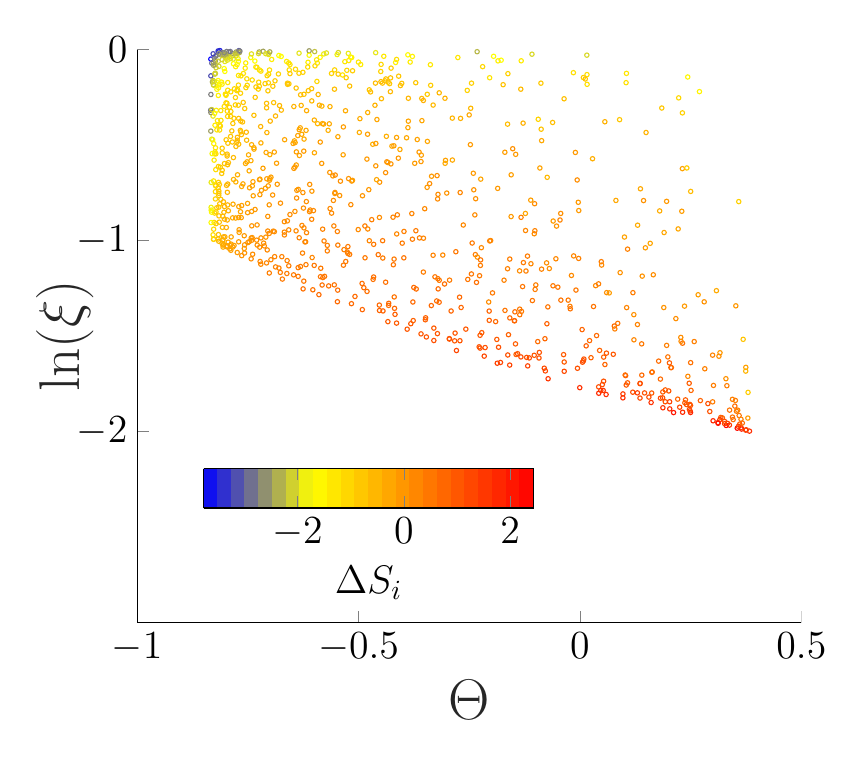
\begin{tikzpicture}

\begin{axis}[%
scale only axis,
xmin=-1,
xmax=0.5,
xtick={-1,-0.5, 0, 0.5},
xlabel style={font=\huge\bfseries\color{white!15!black}},
xlabel={$\Theta$},
ymin=-3,
ymax=0,
ytick={0,-1,-2},
ylabel style={font=\huge\bfseries\color{white!15!black}, at={(axis description cs:-0.05,0.5)}},
ylabel={$\ln(\xi)$},
axis background/.style={fill=white},
axis x line*=bottom,
axis y line*=left,
legend style={legend cell align=left, align=left, draw=white!15!black}
colormap name=mymap,
colorbar sampled,
colorbar horizontal,
colorbar style={xlabel=$\Delta S_i$,
width=0.5*
\pgfkeysvalueof{/pgfplots/parent axis width},
at={(0.1,0.2)},anchor=south west,
font=\Large,
}
]
\addplot[scatter, only marks, mark=o, mark size=0.7906pt, scatter src=explicit, scatter/use mapped color={mark options={}, draw=mapped color}] table[row sep=crcr, meta=color]{%
x	y	color\\
-0.815615823959797	-0.751791896281566	-0.786206554212047\\
-0.353691213391123	-0.265793202087476	-0.415471450363833\\
0.145856531298344	-1.79741473363579	1.08187343936985\\
-0.177977103344908	-0.054791634422772	-1.69938419315672\\
-0.534853750313016	-0.550374617107488	-0.211642420493991\\
-0.812072689011563	-0.399601823669643	-1.06906005464695\\
-0.823317630070181	-0.74324904010812	-1.05355903473029\\
-0.00383194379160456	-0.798975035377094	-0.0680467386197532\\
-0.806263781587902	-1.02310050087202	-0.38068419444319\\
-0.346850283526788	-1.50421524567005	1.09176179019891\\
0.0603045266803143	-1.27212354108448	0.125301925231952\\
-0.660837993960462	-0.896138338619665	0.162577304778169\\
-0.829419515090726	-0.470944428810399	-1.65677564429756\\
-0.807549671152939	-0.930249059146022	-0.562822088285484\\
-0.726445366638569	-0.20610574576606	-0.964390177447218\\
0.180038605280998	-0.844171277178971	-0.373808754299229\\
-0.81583428045276	-1.00301505731869	-0.601096061011719\\
-0.82178209222782	-0.910691464401183	-0.844047816450217\\
-0.830052234962944	-0.168801296733278	-2.34232698971876\\
0.231610469850911	-1.53696327001097	0.629473863449612\\
-0.724188357195897	-0.191727701039699	-0.875697094821136\\
-0.58162153263071	-0.386968494113125	-0.343552960162146\\
-0.780382647940425	-0.204609350350659	-1.08015862307043\\
-0.42660481906617	-0.0962403036488911	-0.875471832867204\\
-0.734157511597854	-0.0593198962577055	-1.69475864445509\\
-0.63940727502809	-0.736524236857563	-0.0531718355541591\\
-0.641214673182448	-0.94864541362279	0.198679556498002\\
-0.77484499862017	-0.484910424643485	-0.588214894455858\\
-0.479208089449945	-0.938744328380655	0.19520312232775\\
-0.699491696396937	-0.37370491426617	-0.506096050735605\\
-0.458501682759224	-0.365460925871844	-0.274999724455774\\
-0.741253532012179	-0.922261944307723	0.0013203490905119\\
-0.634001427875923	-0.41859828290064	-0.271519975753587\\
-0.303666458568016	-0.579380690913824	-0.196775342472619\\
-0.36335632873425	-0.53600689948737	-0.0703545173736389\\
-0.547882397378657	-0.951933809728898	0.340565839500389\\
-0.606024593071701	-0.203819346357847	-0.730010607084221\\
-0.704492152165879	-0.0190696015214708	-1.92590874667715\\
-0.128460178114425	-0.384345111701965	-0.439355810657609\\
-0.769853805493069	-0.942809477781677	-0.140377925063435\\
0.359475008371502	-1.91568046386217	0.522792365934315\\
-0.5532663498938	-0.747470521976626	0.0437976668064345\\
-0.520131101119458	-1.0718662483253	0.441015537709008\\
-0.743051680989002	-0.580833263032974	-0.364489308746227\\
-0.722653941532795	-0.677903460318987	-0.254942446717799\\
-0.586810199705257	-0.0397634690495619	-1.5758817234613\\
0.23683469350999	-1.84894922012286	0.840281616522671\\
-0.781508748832266	-0.359102191279328	-0.825215445353747\\
-0.708825497507374	-0.538097809395571	-0.279058941994461\\
-0.278926157674583	-1.57519446392014	1.28611933843724\\
-0.0617333428361251	-0.380958663291514	-0.663478553519151\\
-0.697937699709011	-1.09970214634725	0.251191094068572\\
-0.806684814237561	-0.872279555088008	-0.554426643794009\\
-0.594780859888407	-0.0526922739940982	-1.33915957723416\\
-0.554853686242317	-1.23142872782227	0.557197783354534\\
0.300568480799508	-1.94318020499565	1.76446146057585\\
0.353477635311851	-1.89294156208446	0.453238456472659\\
-0.53295023284201	-1.04682432817084	0.343252294115541\\
-0.743542860978541	-0.0407649253951749	-1.73263119601578\\
-0.225623955012265	-1.56244349636643	1.12281089481341\\
0.129832001540029	-1.43905969156304	0.289554496807595\\
-0.816001157273586	-0.010043019577085	-3.26145429424616\\
-0.722856266467171	-0.758953847187861	-0.100278986909286\\
0.248575386094584	-1.89135568381677	1.4143138729181\\
-0.742624198042372	-1.09508847815579	0.144189856304151\\
-0.0148396130003385	-0.12020194614618	-1.19570641417481\\
-0.813140973166755	-0.00437199116308036	-3.4885588179505\\
0.0775033604602725	-1.4469534154687	0.664164352107472\\
-0.78243357108914	-0.679397864055594	-0.507443433920045\\
0.135578140442364	-1.82419125710221	1.17801073446263\\
-0.600212716846762	-1.12954710447568	0.481496461433941\\
-0.567495712481718	-1.23699945049881	0.580426282693952\\
0.321654128812483	-1.92803166320307	0.818696120454435\\
-0.58233097672791	-1.23219388456293	0.604900447229966\\
-0.80084021359983	-0.232327856477006	-1.24807318821205\\
-0.132703981659564	-0.0579920635223283	-1.38592055588697\\
-0.22563986671789	-1.49551253811692	0.954065305792851\\
-0.756043633524512	-0.0964568416180298	-1.31948266740265\\
-0.522556485259594	-0.674970079621221	0.0338072267725698\\
0.044366784834641	-1.57470244826723	0.829758644388151\\
-0.110706872657844	-1.12080196157059	0.223560260412818\\
-0.33513780872737	-0.662610023308604	-0.0829040591852886\\
0.00772281393527408	-0.145708000818994	-0.918507696711938\\
-0.16350744658619	-1.1469710061601	0.339929904641019\\
0.0158881921279249	-0.130325074788261	-1.17543852160907\\
-0.623706913130579	-1.2118674078983	0.498570457485676\\
0.177744509503947	-1.63065380774016	0.682455107204125\\
-0.797827735384003	-0.00926542806724253	-2.80351350087885\\
-0.547097123931936	-1.25889753103685	0.631396640185171\\
-0.733764631527641	-0.836633450892284	-0.045157769772607\\
-0.662506018504248	-0.0614373039018803	-1.43311304809362\\
-0.275776496245414	-0.0408397196997476	-1.30087041833516\\
-0.107445581772625	-1.31356769875679	0.53568107312034\\
-0.700353935278479	-0.549262698138716	-0.386114676834256\\
-0.350634474632121	-0.832626816726356	0.211924178485134\\
-0.323580617428282	-1.31566447543468	0.650501471954776\\
-0.57799050637001	-1.00150157505083	0.332639673732065\\
-0.773772489900716	-0.0185961411149292	-2.25546613098716\\
-0.722409611937061	-1.10900191203018	0.216756290993977\\
-0.598389777863771	-0.0845587233032599	-1.03540087212686\\
-0.689508942986178	-1.0836552049374	0.292734904017061\\
-0.585430427468183	-1.14433857487938	0.45323619793125\\
-0.0450427662986914	-0.891653363727011	0.303971507316679\\
-0.422209129874237	-0.877131631219605	0.285331154373372\\
-0.681003098656998	-0.126903768824193	-1.00408454589842\\
-0.437206058654507	-0.45355893940109	-0.39766397919439\\
-0.783124340981706	-0.0488647542029979	-1.93260503808817\\
-0.833580543142595	-0.136939233532645	-3.13320917406572\\
-0.623326853904739	-0.233348103260341	-0.739471229953357\\
-0.00902128437781258	-1.25862679872458	0.467476524947571\\
-0.824216791146621	-0.395434184322077	-1.41171876905941\\
-0.806534143325005	-0.0242449127886784	-2.46170695137632\\
-0.588521530241238	-0.290383100099856	-0.457918275348835\\
-0.337119327870091	-0.18638344429259	-0.890789254604274\\
-0.824936105268584	-0.545382946417721	-1.31087768840303\\
-0.823272965983909	-0.709262866441175	-1.093955148123\\
-0.690193005197009	-0.952831132121466	0.0910852938245944\\
-0.0806410996236866	-1.66785891970597	1.20310579466955\\
-0.0434602084186018	-0.857384966846449	0.098048929822254\\
-0.760473460837838	-0.275986779159049	-0.759649008056135\\
-0.269703027378322	-0.359496348507047	-0.412677123911569\\
-0.515475533632127	-0.0405582232381783	-1.48422592084729\\
-0.171471504510937	-1.2069554896374	0.317894129705854\\
-0.770180820470196	-0.00439164160780345	-3.00553501700784\\
-0.417690623119379	-1.38594337748013	0.885121054261791\\
-0.822243530505892	-0.545182185853895	-1.18289274007817\\
-0.769357607965275	-0.0154637939311217	-2.3362203192248\\
-0.714408717037977	-1.01261977405381	0.0795501484502908\\
-0.788625180406414	-0.220430653399282	-1.11551126083134\\
-0.433823965152048	-1.42393215837415	0.927621790603275\\
-0.322719881733018	-0.659200493524618	0.100508974910604\\
-0.221809436335176	-1.48167331766636	0.916123850604952\\
-0.449433091830009	-0.167247102693201	-0.595836791327825\\
0.379189055714994	-1.92897437114968	-0.059510146331925\\
-0.438369303816996	-0.153037206178149	-0.782479644100621\\
-0.614208596332641	-0.0657938110149402	-1.41360936670408\\
-0.0753380788600035	-1.1162558661308	0.123101911669376\\
-0.619541211320687	-1.00562459036031	0.189116390975354\\
-0.777248082560873	-0.692221617917253	-0.459763478078609\\
-0.679812964786896	-1.14326924960411	0.358100576928417\\
-0.828922647236075	-0.160693304096567	-2.18706987726078\\
-0.640985741499268	-0.200680026842741	-0.725853198529947\\
-0.796500815587047	-0.0435644630944353	-1.99337767787597\\
-0.643757074969433	-0.614388658798311	-0.125395383482026\\
-0.803371492306912	-0.297008188166552	-1.16951134470545\\
-0.317882952236499	-0.225654209353703	-0.555975071287847\\
-0.820367027132936	-0.827832820237345	-0.862907369197615\\
-0.452398371173867	-0.693644853785061	-0.00189821074870469\\
-0.710413426978224	-0.725592682463908	-0.11798901889625\\
-0.370920162041577	-0.172756073233246	-0.787832306736948\\
-0.123244768406764	-0.857453804067225	-0.259848703018206\\
-0.578633959273803	-0.0221373878752133	-1.83756507667459\\
-0.305855250018616	-1.22680326629256	0.653952587023636\\
-0.634445084947108	-0.0179321766101319	-1.90674238385676\\
0.346016272124015	-1.93676776658374	0.661271438588738\\
0.0155220048535217	-0.0284236866087961	-2.0178046816458\\
-0.70778649095597	-0.30415020044736	-0.636455978457824\\
-0.282074827389965	-1.48386068829103	1.0147379067439\\
-0.132051478994889	-1.37017293660425	0.438988116613552\\
-0.358963381766017	-1.48813059387999	1.01862456317335\\
-0.0355752695541633	-1.63530363205532	0.951074531022663\\
-0.572678854342426	-0.0169691612872633	-1.9343530404214\\
-0.0265788358821584	-1.31127068672497	0.47442929483051\\
0.368565132006306	-1.51664530412869	-0.748617839041625\\
-0.640759086703992	-0.603592074622351	-0.173628731330265\\
-0.339492144380444	-0.7010214155435	0.111189306803487\\
-0.690325530361418	-0.535793253099448	-0.245178070208493\\
-0.618636238955178	-0.422385515072629	-0.330023274579439\\
-0.556867892868995	-0.789358790538408	0.128171412345169\\
0.331767966804967	-1.75956792688987	0.390305378017145\\
-0.782659045318893	-0.5648346634279	-0.601306215709615\\
0.158655670998188	-1.01387878044427	-0.268389150772325\\
-0.594019335581112	-0.16612765878314	-1.07342778329713\\
-0.377285628256839	-1.32108573468236	0.722774586649351\\
-0.731710338579631	-0.195104984758855	-0.859519229599732\\
-0.82626875173508	-0.578347004160909	-1.34121952920319\\
-0.667040179317935	-0.47126158324253	-0.26230681456689\\
-0.806079645387252	-1.03349320886839	-0.369870846310643\\
-0.335746042381284	-1.33975659670445	0.738661005811036\\
0.250855345445409	-1.78409678547009	0.765414237572921\\
-0.599748300643108	-0.539580388464565	-0.296824675636832\\
-0.379782033226106	-0.857907041950972	0.269158881778216\\
-0.362383166655342	-0.98554081945812	0.37315877065094\\
-0.586550028332358	-0.48354721469004	-0.116446656306444\\
-0.692651123759493	-0.949929717092705	0.162978139364782\\
-0.516073612703967	-1.32995694384273	0.736197765428753\\
0.0374607421488466	-1.49695805947349	0.735385256277613\\
-0.657690735119129	-0.943459932183975	0.1662530972279\\
-0.674486023841057	-0.316347956108047	-0.56952867352832\\
0.0598038069654021	-1.58894108183443	1.00090047513401\\
-0.740414063187212	-0.983772074660838	0.018553560195273\\
-0.827443032170591	-0.992264102633094	-0.982510105413489\\
-0.802712188291976	-0.887354508655696	-0.477642785408967\\
-0.41251852261145	-0.8646475659816	0.318714692327658\\
0.0119951403041063	-0.153165996443407	-0.7747831775894\\
0.140605678517606	-1.18564206144602	0.0536191542092135\\
-0.21622748053812	-1.60461601673388	1.26571026371994\\
-0.66198368455576	-1.17188110978254	0.403374365095042\\
0.0354381162354974	-1.23552829106602	0.244468822378231\\
-0.747132161757904	-0.634277183121686	-0.337830482306248\\
-0.56457312238105	-0.29793015247581	-0.456777857012734\\
-0.617932897411427	-0.795235426852084	0.0817973585936764\\
-0.436190040844512	-0.587005209102523	0.090832035401903\\
-0.785104803486222	-0.0187061559209944	-2.42972839854061\\
-0.634101191018956	-0.984624169716577	0.267686887209579\\
-0.776327131454754	-0.0118124973756453	-2.47418529950229\\
-0.163561621389002	-0.38970083247339	-0.639064051303048\\
-0.558080009967986	-0.660651347752944	-0.039413333347828\\
-0.095361477446686	-1.52845795140212	0.679391755378611\\
0.104088771159968	-0.172557456538991	-1.20653891689849\\
-0.703264327306974	-0.0247862379337576	-1.95874634920087\\
0.249712511200362	-1.89978061980348	1.83171354227553\\
-0.0917978273984108	-1.58527742235291	1.05668657075936\\
-0.808496570220655	-1.01305088269719	-0.42556884032278\\
-0.515369852911581	-0.687707648259663	0.00204534250788926\\
-0.197541208198233	-1.27339168843515	0.462963260537441\\
-0.789042468662654	-0.454127333318282	-0.78130598151299\\
-0.821265558946695	-0.317433088836557	-1.44166623524017\\
-0.74848075784871	-0.550546574401445	-0.397483469414188\\
0.160694219264153	-1.84748370391272	1.61426910629319\\
0.206432446537561	-1.66473729472084	0.630336671648032\\
-0.0499702842939083	-1.24340038971226	0.509946491162994\\
-0.819507362047613	-0.171415620484391	-1.7114151173509\\
0.195663825187044	-0.79398962969226	-0.0468499106522139\\
-0.479385202749917	-0.328758183382831	-0.424950568691279\\
-0.00273899817676893	-0.84219693187004	-0.0709754641973203\\
0.0139381371702962	-1.55087449799446	0.887194965656065\\
-0.327462848565373	-1.18945323717426	0.526093732396522\\
0.195741100301473	-1.54833767161831	0.358809663008724\\
-0.0529155375595358	-0.923525709753119	0.0557248766715468\\
-0.536252348767812	-0.132207945596974	-1.30505726825534\\
-0.158410009303947	-1.40460143324255	0.74376133460196\\
0.0969814263770069	-1.82306451037536	1.67275896155455\\
-0.611623834223752	-0.00572078458855534	-2.5031022703857\\
-0.788852361475961	-0.349176784802529	-0.90548504116823\\
0.288942223972256	-1.85320713971061	1.12285375668811\\
-0.397433395224218	-0.951679824649486	0.357292913747109\\
-0.475717165682353	-1.00022067456355	0.271192558449105\\
-0.118503325097816	-1.08066372371927	0.417430475872455\\
-0.816403527047434	-0.694472519483665	-0.91130254756827\\
0.19263323480462	-1.78161954149928	0.884497148521612\\
-0.833694647370128	-0.426161076006084	-2.50331652693833\\
-0.014195218996776	-1.079919019313	0.242908665894494\\
-0.250173575961959	-0.341395444051408	-0.298663284274829\\
0.0811747390283365	-0.789294302925924	-0.298372543796361\\
-0.680077898795345	-0.0301920029931785	-1.69539889872562\\
-0.705026339135218	-0.872831066697881	0.031035458038271\\
-0.401401792030478	-1.01298234665165	0.42939402452442\\
-0.0369622859734415	-1.59676130842988	0.947769101340988\\
-0.388670849207152	-0.0267129343832562	-1.63612587139618\\
-0.331676503874532	-1.07640036364057	0.308500774783429\\
-0.554404764610295	-0.206643016588223	-0.653990580200736\\
0.281902268224049	-1.67087186520154	0.347734808074999\\
-0.000478519698441593	-1.7697961048081	1.65414023450906\\
-0.617477730631874	-0.319240032505877	-0.391158981590522\\
-0.127754327103229	-1.11480943015365	0.434007235155371\\
-0.329973920817246	-1.45777706795369	0.958999305311847\\
-0.0781219735275434	-1.68208099868995	1.25606079668031\\
-0.765569756305001	-0.136788587844748	-1.18948823980625\\
-0.783786748270965	-1.03297662787795	-0.151553200968365\\
-0.73923508637615	-1.07104555577667	0.123045388714208\\
-0.740286243887524	-0.158495417571482	-1.07972010476109\\
-0.101295166716318	-1.25524109690561	0.406495774485697\\
-0.815741316421412	-0.763317907844296	-0.820651741822354\\
-0.235584620767656	-0.78024032549272	0.0969053259489568\\
-0.461138078212019	-0.608171125216398	-0.0417370605874556\\
-0.465874678121579	-1.01922099325563	0.465944193626027\\
-0.820693101608693	-0.0290009544527064	-2.6820669431511\\
-0.345217674015296	-0.720852119386072	-0.0445208414905285\\
-0.70179790725707	-0.812330546715615	-0.034484093448065\\
-0.706507276239246	-0.136084805627235	-1.04562186656116\\
-0.657585591266666	-1.13164664948985	0.393611959457074\\
0.0752555037705165	-1.59502082293501	1.0054943346484\\
-0.783526450322189	-0.808889316265475	-0.347827734833352\\
-0.32062270632238	-0.757335177798089	0.150504043728703\\
-0.833628046173311	-0.0488787408013944	-3.76384622481204\\
0.355119174266023	-1.98198149114583	2.23526057633657\\
-0.243462776502082	-1.01222203841213	0.456117240396471\\
-0.736164244162136	-0.520546928954253	-0.381969536258171\\
-0.815573774853502	-0.824262583017203	-0.744779116421447\\
-0.0719462800380621	-1.72305723036879	1.55373004182723\\
0.271937463665737	-1.83756144938801	0.835987809721666\\
-0.812293489406184	-0.6154877811095	-0.87921147611145\\
-0.179508501565259	-1.63784491344749	1.32840732284303\\
-0.61073942309441	-0.848082675060926	0.144859377001075\\
0.269874043984781	-0.219438233388692	-1.5303827289416\\
0.056406387404218	-1.6486273381102	0.790155720966949\\
-0.419453771657676	-1.2946596994992	0.563140661360987\\
-0.0225630040546525	-1.34387539523032	0.36078248624414\\
-0.817210885415865	-0.0064161481590088	-3.37265980631814\\
-0.233681357209531	-1.21845538582765	0.617727610185481\\
-0.162998494584049	-1.59864888435608	1.10714016939416\\
0.00575248638248715	-1.63630469934419	1.13846752090258\\
-0.378466123275081	-0.0350873133248537	-1.50240172189427\\
-0.0358783939142142	-0.25693039404663	-0.672330731578184\\
-0.092546516328857	-1.61441351794048	1.09519488457132\\
-0.826887795088689	-0.186216990195012	-1.91638151710515\\
-0.414202615272097	-0.459554088205268	-0.243023499481993\\
-0.793132455918861	-0.0124640597095462	-2.68145652934508\\
-0.0875784561984232	-0.416169061970751	-0.731371411594932\\
-0.776165413949159	-0.0318188657796854	-2.02254778546347\\
-0.791522260249876	-0.300941633228025	-0.991782513116153\\
-0.723745134131339	-0.680616431341407	-0.153634595887592\\
-0.466018372033599	-1.1902905487078	0.61804444094212\\
-0.452755498755701	-1.36570392634831	0.809771441576698\\
-0.542667662603685	-0.763512800679567	0.0156771098289565\\
0.318029430189389	-1.92577178824542	0.878928527349875\\
-0.721066057131645	-0.402331174640643	-0.482064345422074\\
-0.545785207580624	-0.014815824637078	-2.0431033488302\\
-0.406546652679447	-0.522320202215603	-0.307493524080719\\
-0.498270381453693	-0.433124194110695	-0.36937061174204\\
-0.0355783801837863	-1.68402979619149	1.22626118202254\\
-0.79547298363631	-0.703365381273812	-0.546403939655635\\
-0.47304102795463	-0.220994923819089	-0.61281710884825\\
-0.353462751760565	-0.98707527130975	0.277989029732526\\
-0.825204643347296	-0.855335072539862	-1.04638010326491\\
-0.766636501379329	-0.227611025130168	-0.958370452024507\\
-0.827422862321248	-0.0682360731379193	-2.41969026205359\\
-0.624490913339131	-0.829186043017845	0.090078136894194\\
-0.8242442725839	-0.127508716606434	-2.09397950612319\\
-0.214223989403997	-1.55962828554766	1.12766887838589\\
-0.757475343183628	-1.06447264277168	0.0474221730081449\\
-0.805382223272092	-0.980287847711795	-0.441418315347135\\
-0.520136194823258	-0.190365027908127	-0.696545283449037\\
-0.822520914470334	-0.627817795284401	-1.14814796246089\\
-0.79694734705789	-0.556555229573677	-0.659877700131803\\
-0.824174624628777	-0.535355551055035	-1.26279081167194\\
-0.136362355294676	-1.15821187276601	0.167619087214239\\
-0.453121604981571	-1.33721134899867	0.743586316663848\\
-0.630890856356147	-0.236144014913908	-0.623379244362089\\
-0.564399043343785	-0.831731930943123	0.188777665121691\\
-0.576821578797494	-1.18679176760678	0.506025180142184\\
0.231828988799073	-1.89850794229697	1.75648412450188\\
-0.566162917933827	-0.388070428442978	-0.316268891198331\\
-0.145155484958737	-0.547900315647675	-0.0859901939666222\\
-0.358269759201713	-0.552107604038762	-0.167577257804316\\
-0.808247319645941	-0.180388598775979	-1.41478349584073\\
-0.382051872489021	-1.43481287335725	0.943867719822606\\
0.0217109595975533	-1.52328540866624	0.747258916488096\\
-0.788504216934351	-1.05038020882061	-0.154221541020639\\
-0.467961156500522	-0.495095860151936	-0.392130743488082\\
-0.831453686215221	-0.0701411781805013	-2.94774585870149\\
-0.778929712180471	-0.0211297893024436	-2.23119977299891\\
-0.809471543620717	-0.169638932010825	-1.49149104964741\\
-0.599971585485796	-0.368421981828995	-0.414591411410928\\
0.103114043304299	-1.70666642832066	1.006157881117\\
-0.697832840939158	-0.66737676461429	-0.185544701062885\\
-0.770728513359794	-0.359805961177268	-0.701517235852629\\
-0.185139518849672	-0.0583935047796798	-1.45429316342795\\
-0.448341057882606	-0.256430762559693	-0.577095415945458\\
-0.646143836616393	-0.297434895197013	-0.488899695001969\\
0.121884548312757	-1.51930558817941	0.264126881916818\\
0.299599626878469	-1.84394273650814	0.439513857641035\\
-0.706262844522015	-1.04847942738361	0.209228691592857\\
-0.634580429640956	-0.123066315360487	-0.976825614318679\\
-0.00629758608609921	-0.682044833546891	0.126196261581652\\
0.316216195307413	-1.58691301692543	-0.05478036215696\\
-0.707832465671564	-0.280593436273266	-0.655738783528945\\
-0.491178085042356	-0.764762437876735	-0.00234286697152022\\
-0.766637353522474	-0.848384252545206	-0.259656642458341\\
-0.732045535163216	-0.0905620823330928	-1.39274303645873\\
0.121650294920406	-1.3874588103304	0.0815926448618805\\
-0.741360379435427	-0.846885702852289	-0.0968526008250297\\
-0.815316161023369	-0.870176889540313	-0.705980004891571\\
-0.526513525367911	-0.10776910933868	-1.08834565491695\\
-0.815472287384347	-0.0870659920379975	-2.02679380110087\\
-0.678517094580967	-0.292364413922714	-0.588057312783619\\
-0.647876410052014	-0.490719290937438	-0.212211007480737\\
-0.771364455618808	-0.0610245687523876	-1.61649153679259\\
-0.263535227693433	-0.918020819295883	0.204829394328685\\
-0.824500832913978	-0.0781386060259953	-2.32515377459385\\
-0.524054048022333	-1.0309985343468	0.459538504240126\\
-0.222644839275736	-1.03682728004365	0.204043146608988\\
-0.814605070933888	-0.902883068293914	-0.694962434931425\\
-0.383445244737052	-0.0645566115905956	-1.40442838510557\\
-0.169607121470432	-0.53688259279992	-0.122316611229196\\
-0.810766879470692	-0.370113025863339	-1.18385065648364\\
-0.816519627220251	-0.967977986463827	-0.690291888409776\\
-0.236261314826662	-1.07280432219022	0.394367935713893\\
-0.676795627003151	-1.16628867289904	0.409099010867467\\
-0.449146328554517	-0.076719816451639	-1.05200256856888\\
-0.0790970424163357	-1.51349180614466	0.740358351548149\\
-0.831476342788286	-0.468312464125175	-1.86719317095415\\
0.337878487107415	-1.88727134832564	0.560008902707303\\
-0.639969399432703	-0.776570950608691	0.0966017428879176\\
-0.799399434582382	-0.238531362814134	-1.24552840663557\\
-0.433295353943584	-0.17009976548929	-0.676320064284382\\
-0.359004266858692	-0.585468671133789	-0.0688286431782785\\
-0.617531697934796	-0.958182627114814	0.25842097809634\\
-0.461840916217014	-0.174657069120326	-0.627706819945371\\
-0.356913740536825	-0.371438712143613	-0.274194483871039\\
-0.148147356560586	-1.41953452390895	0.499150750554466\\
-0.570648283438019	-1.05357033404189	0.372427036673042\\
0.236115960071116	-1.34277647662606	-0.0606012734041439\\
-0.158687602330568	-1.65140693709325	1.33377681485442\\
-0.801885350439571	-0.980017873666545	-0.361697382764001\\
-0.774383564554783	-0.0779385828465559	-1.57633017490356\\
-0.738527836313372	-0.691200911678365	-0.214977313849151\\
-0.373210486059248	-0.594739737883294	-0.0895162800755062\\
-0.144376689762434	-1.59595945864713	0.910986935891914\\
0.35626027620702	-1.88757777335627	0.310042463919192\\
-0.625737284131629	-0.747998087839512	0.0473254441360799\\
-0.462977110053367	-0.290785324571426	-0.465487725549489\\
-0.133343903132611	-1.60879198478906	1.17642777554818\\
-0.548416054062408	-0.0252664069839056	-1.80282081469575\\
-0.610338251823958	-0.705346537380661	0.032271216386939\\
-0.776933838693546	-0.506577226553736	-0.605556613442881\\
0.00887863246965237	-1.61987044608962	1.08681546438234\\
-0.799442231022511	-0.278106272589918	-1.07386655342287\\
0.192679126920496	-1.84352837214481	1.05056627036014\\
0.24369176677078	-1.71038218503726	0.217980218324749\\
-0.34488648656166	-0.233474482975496	-0.874413988019553\\
-0.661377380158141	-1.10437308595382	0.329514067025645\\
-0.155323967854351	-0.655155494226543	-0.14311332386226\\
-0.739984348060574	-0.713284814225974	-0.253569321331007\\
-0.604875722241381	-1.08826129771218	0.26375180046346\\
-0.074639423252983	-1.43504126843516	0.854986596009233\\
-0.741499024951836	-0.497376705982711	-0.423291810276112\\
-0.629647078175029	-0.291804650168763	-0.481235616883162\\
-0.703108585442548	-0.128223192970663	-1.04763217612815\\
-0.609411636572714	-0.839480972843835	0.140709667898605\\
-0.444853123800788	-1.36799709779011	0.820831933289982\\
-0.828721261700612	-0.347399775509108	-1.8672345946986\\
-0.0103758303459207	-0.537960463673413	-0.0575036332568204\\
-0.794064000749799	-0.843315245939814	-0.404456218731167\\
-0.151925232425589	-0.518401193780781	0.0821472537423116\\
-0.736292871591788	-0.512917289566326	-0.416286906028691\\
-0.69619011359818	-0.0509538583643941	-1.41114215842232\\
-0.737954544057756	-0.764945488797162	-0.193596661902242\\
-0.808061698729132	-0.515579809643775	-0.862896794874411\\
-0.82412376423082	-0.123461642792868	-2.04997165708575\\
-0.32997145588651	-1.52285337936829	1.13224588014678\\
-0.475748148174238	-0.210082279186305	-0.799334095423911\\
-0.552774784321115	-0.656168199030396	0.115838705244532\\
-0.693596211068506	-0.191247431858818	-0.802128910770044\\
-0.754808753272025	-0.0693388200760559	-1.46538317369944\\
0.363688679517279	-1.93507346513068	0.318722714624364\\
-0.773357694006267	-0.208514836093485	-1.07972562070629\\
-0.605421831552121	-0.740533544071161	-0.0431929675780832\\
-0.387548202356482	-0.254216248276965	-0.519889710631613\\
-0.605875531761924	-0.887908296445401	0.254285453740792\\
-0.455603204585875	-1.07308084956502	0.569284711577961\\
0.36394250291553	-1.97897383473841	1.42426913551706\\
-0.321898943110175	-1.48663089216352	1.01746896348207\\
0.231263640661843	-0.622690195940963	-0.187531151867183\\
-0.554078121126924	-0.105635724548848	-1.02617708591628\\
-0.424649866977104	-0.504760376423269	-0.307118249992294\\
-0.500801012470053	-0.941816303576009	0.198948175674948\\
-0.819907123520636	-0.207161912327516	-1.63251408175461\\
-0.623761298282455	-0.531016780783907	-0.0905173914294646\\
-0.701644058506043	-1.16921377741826	0.380109742356054\\
-0.683685418986683	-0.704571842005619	-0.0831956479947783\\
-0.591260907824386	-0.234440546195075	-0.550087300014492\\
-0.807392932094197	-0.0155563739670936	-2.68782408627286\\
0.351965041594408	-1.34108898001853	-0.0341414872596898\\
-0.625282484159585	-1.25242181640031	0.618948545800606\\
-0.770719962751886	-0.494748531019649	-0.633655694995511\\
-0.555766823536657	-0.92297204459149	0.282085671456723\\
-0.271060113024285	-1.52395152929763	1.03706875806213\\
-0.81698565218474	-0.722776785324888	-0.904290145799563\\
-0.771310683925868	-0.185061687845614	-1.06959053571583\\
0.22998789684617	-0.845910502132218	-0.127618942027704\\
-0.294873184197152	-1.51515962011587	1.01017425948092\\
-0.0865457028874999	-0.476162920015855	-0.304116156408852\\
0.149262986388608	-0.433475947070646	-0.473445141763454\\
-0.833575890209166	-0.328922915484742	-2.58106403996981\\
-0.295116603900023	-1.51283659503747	1.06576891618896\\
0.119231393971621	-1.79340444414932	1.15291077985132\\
-0.741947433179901	-0.0220662015409756	-1.95625412977887\\
-0.688710174491542	-0.163044172186977	-0.878748232149526\\
-0.397777520876678	-1.08990461723888	0.527560025003242\\
-0.712908795221401	-1.02751600811604	0.144229685199009\\
-0.19504538161633	-0.0344628797362706	-1.69773111665479\\
-0.833021760465319	-0.825499180320666	-1.81417451875316\\
-0.831973242720666	-0.850867596380207	-1.6192030566846\\
-0.239861198812824	-0.73352495563306	0.0496619161226436\\
0.139616510666993	-1.70412924036226	0.726107201433271\\
0.243452427376684	-0.142863114574435	-1.58317965670113\\
0.299561445933665	-1.59953096418115	0.290162381619438\\
-0.782566394320767	-0.0732385568626987	-1.67955577623397\\
-0.827407067828624	-0.687220284166806	-1.29199599300188\\
-0.807775115903311	-0.539873221554131	-0.91003748762023\\
-0.13306973699826	-0.877681339607478	0.339167200288077\\
0.0562016210049955	-0.377240884887284	-0.457937701646717\\
-0.320222820068675	-1.25249527884306	0.704549986458361\\
0.184794381628849	-0.305285657041601	-0.78671061849278\\
-0.720585164441414	-0.1119550851836	-1.14105469208747\\
-0.135958147840232	-1.38757452741867	0.51725735163281\\
-0.823250737623992	-0.781531178667624	-0.995611845528342\\
-0.818717279621128	-0.371577203635635	-1.26638563037735\\
-0.74249250012416	-0.986088771352503	-0.00125066673402651\\
-0.402520280773168	-0.17602757957641	-0.761990968813954\\
0.379613453577909	-1.79437627916318	-0.893636977732219\\
-0.654936415029577	-0.0774921303722034	-1.22589998227328\\
-0.720536924834455	-0.488041223147629	-0.397404183148817\\
-0.581101697006458	-0.93961521862318	0.314893495838746\\
-0.77826465139258	-0.288916673131235	-0.934461627611977\\
-0.795436888596271	-0.171848582287597	-1.26788354418319\\
-0.527983934657091	-0.146577284391696	-0.874588038788967\\
-0.751489112951752	-0.186103367804979	-1.06768636891243\\
0.249675159031492	-1.86256754158157	1.04583387586546\\
0.0283676796095997	-0.570853116923789	-0.399032580377505\\
0.202752319702565	-1.88085728161933	1.66597361487612\\
-0.815266977022925	-0.0201206944535044	-2.62135288209955\\
-0.55355735632288	-0.752861469800901	0.00755568212543913\\
-0.823491152061802	-0.124340911762181	-2.0801294673762\\
0.0970828570754371	-1.80254133480025	1.44261193394324\\
-0.816038857970783	-0.198926686683446	-1.51751872108856\\
-0.701783174114761	-0.961972764279035	0.167301020661142\\
-0.593183694917796	-0.0698394504661624	-1.24640649684893\\
-0.750736265308625	-0.804909252449977	-0.228476727902604\\
-0.787776083262328	-0.980183110376109	-0.264931376655665\\
-0.806822268464008	-0.997974135025451	-0.423416445182862\\
-0.764089527983944	-0.716110964757083	-0.339795823611579\\
-0.725533775131317	-0.170053749935119	-1.00668935977821\\
0.382814841307203	-1.99736513783441	1.67967484065494\\
-0.827275147110752	-0.939814426856417	-1.06798678590057\\
0.249988188721781	-1.63877472665745	0.599578718132186\\
-0.786269471484803	-0.425138567958144	-0.762955279736325\\
-0.80493568619435	-1.01977451955923	-0.361630171803884\\
-0.67474046952072	-0.0352595093692694	-1.65000156460853\\
-0.70474262204298	-0.215210139940876	-0.814930207796466\\
-0.565074765972613	-0.64273673446326	-0.023310676862648\\
-0.206107465355275	-1.32116808180228	0.154812152794253\\
-0.288349184219686	-0.358212833545092	-0.516429145323039\\
-0.657737004825227	-0.0691583131265833	-1.25725817412207\\
-0.431944931796156	-1.32793671872583	0.768003097342659\\
0.0907960623204381	-1.16730832907632	0.0681241111904859\\
-0.10318528222195	-0.963727498132787	0.130735798104873\\
-0.770600960790527	-0.878615116162374	-0.215293114848532\\
-0.769711898357269	-0.956436141024362	-0.157416020180484\\
0.221804134010494	-0.938531990860301	-0.270068827531609\\
-0.77220275655545	-0.0466760075511679	-1.80790105414581\\
-0.42689215440921	-0.597987124654332	0.022292621180936\\
-0.766208354223969	-0.373391521002977	-0.69262980778993\\
0.311733752177282	-1.9526380653424	1.75934500833261\\
-0.496970643068227	-0.36112089482027	-0.36840741391302\\
-0.410204680503159	-0.567817367547401	-0.0551049520874406\\
-0.777591530243912	-0.0887018465840838	-1.4523974298935\\
-0.561149704385631	-0.124373321524296	-0.973324113157323\\
-0.657293936937286	-0.178346882960181	-0.843197802296816\\
-0.778085958314322	-0.250285867191002	-0.959614837674232\\
-0.811048390159267	-0.0270954056487074	-2.4189008297495\\
-0.378426611689191	-0.992237745204759	0.423425846885229\\
0.10740720317827	-1.74438967306254	0.898783330800765\\
-0.0942459355042333	-0.364243147686728	-0.988417887765669\\
-0.491555388344227	-1.36095180106701	0.799367265334721\\
-0.1229093313206	-0.946752730364094	0.250737741261725\\
-0.773998958453255	-1.0619222724225	-0.0853051155239209\\
-0.755355685436546	-0.59575334890629	-0.380976286048937\\
-0.803549243304152	-0.099047033034448	-1.66408003492238\\
-0.161435060143938	-1.49237117429052	0.853850283985513\\
0.202479328192195	-1.84348583477577	1.35825933868215\\
-0.795950729335183	-0.602290663048621	-0.633276932007896\\
-0.687571613522098	-0.347107074172937	-0.550908527632577\\
-0.102457011765883	-0.806405974877883	0.146340224147596\\
-0.672124254915135	-1.20104196163039	0.45123488975307\\
-0.205068292823507	-1.36859210746223	0.785555211057048\\
-0.0431032326923559	-1.31132586529064	0.559302978355183\\
-0.24675347763066	-0.306589490779813	-0.570552650816043\\
0.0504209903097068	-1.7536556806928	1.2215062225069\\
0.216592607497351	-1.40814553511305	0.128125028085298\\
-0.375264103718529	-1.24511180617111	0.694051946597717\\
0.187057164441684	-1.79219701556881	0.921669771042045\\
-0.523243267308094	-0.0190484215065184	-1.85943798259486\\
-0.376568857401805	-1.4184789598438	0.860866878013146\\
0.205385202719038	-1.66441737881546	0.683249244538368\\
-0.320952353479966	-1.19890994730081	0.504745014662449\\
-0.723765060333321	-0.106240797748928	-1.27080634367678\\
-0.331603232331265	-0.289793172072102	-0.578755876868273\\
-0.667446755776652	-0.970059835173421	0.222177623929122\\
-0.746231112691488	-0.722966294472742	-0.206184284196366\\
-0.476914495099723	-0.732944333238876	-0.0492290267800288\\
-0.821901637679688	-0.0936847663241335	-2.04059928944469\\
-0.63610475947451	-0.73131231521305	-0.0371340655829787\\
0.0852795506087669	-1.4329574740447	0.495563949739434\\
-0.578926343659484	-0.38910089440483	-0.319564063728968\\
-0.825700250088787	-0.0425943439648485	-2.7455437728391\\
-0.644926137350823	-0.477340475246544	-0.339460090643496\\
0.0590069968002279	-1.80548272999173	1.66192537269788\\
-0.288136528484707	-0.57763661190465	-0.31524235114118\\
-0.391656446009395	-0.461139507604523	-0.305688666292248\\
-0.804512015224442	-0.0311053651357639	-2.31215664016106\\
-0.811067159351505	-0.783691842413937	-0.748311021973852\\
-0.440037366688887	-0.163058535305861	-0.715705841394604\\
0.360888336494803	-1.96055980449771	1.04092458778547\\
-0.796839502499974	-0.546812860035768	-0.710622412951341\\
-0.452871079294741	-0.878410878832422	0.141846389051277\\
-0.626577844595285	-1.0648582935594	0.309188866184976\\
-0.814973279022291	-0.184054112065431	-1.53186571349431\\
0.344432308290795	-1.83071669943382	0.365562291282707\\
-0.711214073244593	-0.177503310335262	-0.904152284848208\\
-0.227678501009908	-1.55592710464249	1.06499314544061\\
0.0306217509160106	-1.34484173318907	0.54865475344526\\
-0.438855607940744	-1.2174756186369	0.607338240800578\\
-0.158504574237317	-1.09622142143603	0.389976866642048\\
-0.753617832187303	-0.431766151598298	-0.55328581167376\\
-0.724506326833088	-0.0117425938347197	-2.36836923500391\\
-0.413880211516843	-0.964780078929105	0.223063450320611\\
-0.414223819975357	-0.0508662269985263	-1.16508243349818\\
-0.337751889465896	-0.0784875322165381	-1.33769470465144\\
0.102098942122006	-1.70339598944789	0.624036006184838\\
-0.798096449656849	-0.710538975427349	-0.586124900810642\\
0.228340425269648	-1.52699669924275	0.160194017970944\\
-0.656608481241876	-0.105597670145983	-1.14389226132005\\
0.357613722030392	-1.97258189835501	1.35547397582997\\
-0.390233484977096	-1.46336362543056	1.00826204864321\\
0.181838656745091	-1.82467799809138	1.27151923072464\\
-0.304864685434834	-0.254132962442077	-0.445641018752658\\
-0.631085183110197	-1.13512513829859	0.395431246573379\\
-0.725941553381364	-0.0204514782943958	-1.95768809819384\\
-0.58323601391929	-0.595325159550893	-0.0658816958072386\\
-0.720801958959892	-1.1232318397036	0.207064779443316\\
-0.796214578268281	-0.0333705024793636	-2.05850094960046\\
-0.833919805022372	-0.316537865025297	-2.78650394796579\\
-0.7520569509956	-0.587388980735369	-0.354518996616213\\
-0.764946361651258	-0.879222700598778	-0.175422388254708\\
0.189293846542388	-1.35018684983615	0.0301276554379612\\
-0.823266033991737	-0.0571160856235591	-2.44657376682508\\
-0.813864267144024	-0.3954052860125	-1.14757842495722\\
0.00780382691898662	-1.62931715077496	1.12601119400355\\
0.161974526237316	-1.79780912414565	0.951174061544219\\
-0.687440527317915	-1.13737350461536	0.31238338056802\\
-0.816810776908279	-0.239588585106455	-1.4891751210017\\
-0.244953056950038	-0.175011769014988	-0.9386205182634\\
0.0481293171332916	-1.10989493644193	0.410708679725018\\
-0.703616839327223	-0.17341889649127	-0.936502070178134\\
-0.517486055115403	-0.811278382257628	0.162313656014138\\
-0.237392182446686	-0.865067498667697	0.160539343269342\\
-0.691770547643914	-0.27698869758967	-0.719897235939654\\
-0.224107265187301	-0.677685834478392	-0.241017025851323\\
-0.0739964267108424	-0.668142394873409	-0.574799160070693\\
-0.086707906737959	-1.14895689046012	0.309860989979358\\
-0.771559134852234	-0.290530504337736	-0.897231151025176\\
0.344440093500371	-1.92392366516701	0.552143798146026\\
-0.707848393385933	-1.1166333812842	0.244017964244868\\
-0.203771085440515	-1.00125973097976	0.371847258391261\\
-0.495192239641887	-0.0774607233471304	-1.41224841817227\\
0.202114250546778	-1.63991934522194	0.907049700235637\\
-0.797382935603027	-1.0321795474752	-0.229335861791227\\
-0.546067525499606	-0.127718024044523	-0.888143796380871\\
-0.23170619924982	-1.08586727584389	0.0200674043179502\\
-0.0609138483262432	-1.23628135247079	0.477560744432382\\
-0.0692048896203776	-1.14582112414559	0.110186991770631\\
0.30154527570049	-1.75806607964587	0.396478334670797\\
-0.76395425024066	-0.815937656202018	-0.183758680270785\\
-0.796602698130462	-0.0372928810506592	-2.16150834039421\\
-0.224825561109658	-1.12960191915741	0.404004174288461\\
-0.155525246268125	-0.873730360228447	-0.0682979208456366\\
-0.186774669768303	-1.64174898623029	1.35362489967463\\
-0.00296997596581394	-1.09303855385365	0.338392180219805\\
-0.752840786077793	-0.473774798512239	-0.579027858394634\\
-0.534342395914792	-0.404441683850688	-0.136700554063009\\
-0.728934017520999	-1.02291174998141	0.0547627690699451\\
-0.546821509246653	-1.02313937920244	0.390244630394288\\
-0.414223589089336	-1.43159828611378	0.949999423374168\\
-0.349205431678976	-1.41415015953245	0.870308606717046\\
-0.790153196217264	-1.02550371896695	-0.236864936267681\\
-0.409451568193573	-0.138555948681554	-0.786010041050954\\
0.374543909810801	-1.66338724821688	-0.172043186262505\\
-0.752327272915726	-0.152398894965117	-1.13897952544492\\
-0.802004871133488	-0.11345467262995	-1.64938946565026\\
-0.101838062345201	-0.94804246910182	0.302442107844342\\
-0.485418653249613	-1.08962048621756	0.455804617484775\\
-0.773842741241783	-0.473786718653805	-0.610752144768276\\
0.374377062536341	-1.68291146437849	-0.500155947357082\\
-0.582863228436321	-0.295283823565738	-0.498917792542891\\
0.0535668294202232	-1.60974020145237	0.90018292284733\\
-0.646038408300808	-0.621377534853577	-0.0457477312716809\\
-0.817146885193247	-0.161341022923546	-1.64155920374552\\
-0.720387893589879	-0.98555307355626	0.0694408127322372\\
-0.625722733016082	-0.118214189135573	-0.989913777602461\\
-0.203968326684004	-0.146650586980671	-1.27579387466936\\
-0.701183720892248	-0.683583129947161	-0.147207252050349\\
-0.427799390074265	-0.14751254888111	-0.712242133490133\\
-0.169318600396767	-1.36530381570436	0.537709207834141\\
-0.467160996601915	-1.20268405331245	0.564266132137394\\
-0.761082950142587	-0.702697809308083	-0.315461882394247\\
-0.82269581402505	-0.713626103415877	-1.09587240527289\\
0.165645977589704	-1.17846665815942	0.131329604497439\\
0.105427712836678	-1.35045967683922	0.273577980336825\\
0.0534544179356198	-1.73595243288723	1.11305803698833\\
-0.019267895969459	-1.18225641545569	0.172614465452999\\
-0.0605105509046093	-0.897102471003867	-0.0881439430343865\\
0.0423987879034425	-1.7989914185111	1.74055263918998\\
-0.79223610179965	-0.0371835058330836	-2.03133574558725\\
-0.707123061603379	-0.433842865187169	-0.469061047151347\\
-0.240838903594581	-0.646930944380888	-0.0866142872506306\\
0.315999489890134	-1.93696433012515	1.49525559336969\\
-0.190428194320197	-1.4237449081074	0.739305076753924\\
-0.781202604255364	-1.0252239427888	-0.176881088807161\\
0.0488921122366269	-1.127713613043	0.189466896283056\\
0.187302463147284	-1.87506907456464	1.62428428275746\\
-0.707270193919713	-0.676094316612991	-0.146310598539311\\
-0.794569355057403	-1.00770459534217	-0.295938167671317\\
-0.676385474974982	-0.803475714315618	0.0570423312355727\\
0.119608480183283	-1.27226210141696	0.404893216246046\\
0.163155685032017	-1.6875599321248	0.666858569244823\\
-0.162694049183512	-0.125442496246929	-0.964294615964408\\
-0.816661420152091	-0.611713268282881	-0.989718208792284\\
-0.541008648375907	-0.688389858737481	0.0867907562703937\\
-0.814390537348524	-0.705653147193526	-0.843696210868886\\
0.329631864290318	-1.72288149535385	0.0590829400777176\\
0.200490299996315	-1.78693778445887	1.01998641817686\\
-0.420263582997176	-0.503113175053785	-0.150106874492706\\
-0.37057909048624	-0.947874549152236	0.443890867017377\\
-0.798438961537037	-0.0361827700572378	-2.223513382118\\
-0.673369805102149	-1.08371866689035	0.319866280080902\\
-0.801937820861512	-0.0614810960343479	-1.90855588916417\\
-0.30453520403877	-0.594849403314209	-0.346838571932049\\
-0.421446415870762	-1.12599498046185	0.523386273453417\\
-0.705029512294717	-0.949502639707351	0.143794943902194\\
-0.787710441271031	-1.01827154270903	-0.213369762683321\\
-0.760199518281098	-0.124455286163989	-1.21707366017003\\
-0.445698365586472	-1.00008193778637	0.481546425866671\\
-0.777425527026637	-0.881361603308014	-0.229494077550128\\
-0.715897765485633	-0.620835735269115	-0.197826410483686\\
-0.268412694380552	-1.34993865588465	0.760066034168135\\
-0.770752548662982	-1.00602997166787	-0.117480764060233\\
-0.479720041008324	-0.442428408269408	-0.182409177403099\\
0.31388678252292	-1.60518929606028	0.0930748800094748\\
-0.513757749248213	-0.684021250392488	-0.140237143917502\\
-0.715444056711002	-0.00815091227608457	-2.44226300067169\\
-0.825838619591241	-0.166611105461011	-1.9623450123834\\
-0.733450853847525	-0.249408190628062	-0.782697750722424\\
0.107536920211566	-1.04421971906248	0.340120366423848\\
-0.796580704383721	-0.891616476437464	-0.404364876874597\\
0.0249416828354175	-1.61289173318306	0.831834555772353\\
-0.811179066034043	-0.318686403772782	-1.21310516139768\\
-0.82708712443287	-0.491789756082451	-1.50778791201362\\
0.139356468098757	-1.54031903841865	0.4837083979295\\
0.0661191343316195	-1.2735946423154	-0.0961880224072683\\
-0.804111976864179	-0.851149952219548	-0.534304253056639\\
-0.642472137953889	-0.102109695232132	-1.06372531929597\\
0.240549541700034	-1.85810933297427	1.11657722049564\\
-0.709543265339625	-0.0209412647582522	-1.93202165171002\\
-0.796231765638816	-0.0546394542566496	-1.90915158290156\\
-0.187805073134997	-1.51722531233294	0.959236046637893\\
0.181663790664903	-1.72474760142594	0.708298596721344\\
-0.79658057671368	-0.321510838567806	-0.995449215959591\\
-0.646704186744444	-1.17893708834903	0.432134393134114\\
0.143571257664697	-0.789978358891617	0.0618501231499136\\
-0.826261374836603	-0.904553077857797	-1.07940818383338\\
-0.817245187604864	-0.991260741575555	-0.629122728392421\\
0.337572698086714	-1.9657859186658	1.52290756680787\\
-0.799426777773688	-0.235369025086747	-1.2287150430152\\
-0.795743877992573	-0.349149138859626	-0.966526726075317\\
-0.369792986459417	-1.25294362310424	0.645841823662377\\
-0.580634980243558	-1.19290272389148	0.534829139693172\\
-0.80285399478292	-0.596196608005942	-0.772428182363671\\
-0.29101520950649	-1.3683167995614	0.793096555657081\\
-0.627868971759493	-0.920272645708413	0.207061699362474\\
-0.729666613685044	-0.0921267829995227	-1.23057457240949\\
0.19848915519856	-1.60875579320424	0.55554500514521\\
-0.830800070306158	-0.544059019092942	-1.75576211511049\\
-0.103254674955955	-1.6002436154847	0.985684052962042\\
-0.283062317914305	-1.52448292039061	0.99432311938945\\
0.247104433031006	-1.88342804373195	1.17645129896197\\
-0.827541390479123	-0.992723096790738	-0.9765375154302\\
-0.750682997474454	-0.853205502230049	-0.110422336429533\\
-0.788406652970719	-0.3233840121357	-0.931850914768251\\
0.248061071838806	-1.85717458999352	0.981591636037728\\
0.330150948567667	-1.96756031478802	2.44081687512461\\
-0.321461127982204	-0.781478234674086	0.184754560158577\\
-0.773370360762749	-0.654870312657341	-0.415261184509891\\
-0.797291337808556	-0.280406961231305	-1.02625376486476\\
-0.388540227715889	-0.408038268325928	-0.26022909313173\\
-0.736308844179356	-0.343425831089808	-0.677441197288294\\
-0.631747694767412	-0.409108943777477	-0.309503056116683\\
-0.784047459764553	-0.0296342683041488	-2.11413477992561\\
-0.813531363754211	-0.806803939963972	-0.716547236066481\\
-0.570624300043742	-1.02457813963039	0.3457131361821\\
-0.46099615718735	-0.491034055496504	-0.157664422327668\\
-0.546663515205336	-0.455548120575945	-0.284579651348785\\
0.129739113995087	-1.79690624537124	1.40122428616345\\
-0.146945550415838	-1.37269556454802	0.625481868946972\\
-0.140855696904986	-1.59184774146579	1.09805739504699\\
-0.357281833554487	-0.255221622235398	-0.578119016227101\\
-0.428162921352266	-0.219655173480765	-0.569073073459622\\
0.246684512010008	-1.74667080585711	0.910530286271294\\
-0.254560859270108	-0.212962210287163	-0.979643470599184\\
-0.757422790093626	-1.02193713629538	-0.0220412336607654\\
0.28058367332126	-1.32015392623519	0.071037100746684\\
-0.823105453743665	-0.513345042578444	-1.27056899184619\\
-0.219812071852485	-0.0885858207852806	-1.06401902679725\\
-0.445319239582302	-1.09085229460888	0.428827689463688\\
0.308178276396616	-1.26188058884728	-0.333713354593971\\
-0.614819942010487	-0.0906052631195054	-1.11645228061195\\
-0.815491397236684	-0.740285459812537	-0.814775160759834\\
-0.480899527541006	-1.26584533803813	0.614330945492438\\
-0.832834613336106	-0.694829968366209	-1.87535102830281\\
-0.438910971866619	-0.64365924605395	0.0848291448565574\\
0.227713212393819	-1.50663865407312	0.133957469224827\\
-0.224374566734935	-1.10063297812306	0.518774114309895\\
-0.793959963788113	-0.591204472460293	-0.629527718503719\\
0.0787475857591895	-1.46223878207325	0.354278031606848\\
0.220750125604133	-1.82984052330562	0.809246627902702\\
-0.129580162813938	-1.24042899893689	0.523577499959365\\
-0.719373809904245	-0.736295728812735	-0.122628216211544\\
-0.405496067403307	-0.187612351011911	-0.670711301743204\\
0.365075540072596	-1.98651456414359	1.84745981395557\\
-0.1477233507232	-1.41913498403562	0.801903275754024\\
-0.418802353768459	-1.35437403860611	0.772618862225209\\
-0.318045183091346	-1.32228587741246	0.709596269577963\\
-0.741566273240631	-0.998040206187716	0.0267245669068609\\
-0.783939698101179	-0.386087584094624	-0.803649013882555\\
-0.317793101325142	-1.20742609935141	0.483653667911695\\
-0.654915455955941	-0.863239363248421	0.124198631792383\\
-0.586005077182683	-1.18851587123657	0.518143389125807\\
-0.114450944157322	-1.61412448486876	1.16176223006548\\
-0.00562741918662057	-1.66817534741637	1.10397595733963\\
-0.795696663206282	-0.812819026229389	-0.489582118702661\\
-0.309813305388277	-1.07531905222458	0.209104909382429\\
-0.685252013490185	-0.594333049280814	-0.168852469226953\\
-0.133648124538617	-0.206601873102051	-0.604518659164073\\
0.0422508970747422	-1.76557221675004	1.14582359063702\\
-0.449891129527127	-0.113962903207743	-0.98547007698963\\
-0.56092958957709	-0.85562673606896	0.193007847451084\\
-0.253381453037167	-1.2027219991415	0.519522113042726\\
-0.633611094821414	-0.553971762832487	-0.234195630996021\\
-0.618777289199363	-1.12555572848385	0.405413738209579\\
-0.353641309486102	-1.1643325056804	0.408033223698376\\
0.35106834313464	-1.83672435697005	0.383938875760635\\
-0.387605231453819	-0.374143825561788	-0.242183841043519\\
-0.799849682703686	-0.0225738365520039	-2.42012663945202\\
-0.433812853264993	-0.590610090432269	-0.0839243067761072\\
-0.771201797678261	-0.134824785321048	-1.31905943216231\\
-0.799132357078101	-0.471602135196323	-0.816587163902504\\
0.186753475527586	-1.82312124166427	1.09044314149809\\
-0.802861114847649	-0.821537324176666	-0.527908141623338\\
-0.20488479265668	-1.417304609131	0.861748154915575\\
-0.446086726668045	-0.174567130170849	-0.724861286951451\\
-0.79631266092567	-0.74668053521598	-0.502055390562892\\
-0.704046959068264	-0.712881698065022	-0.124558756980566\\
-0.803097131420329	-0.0156712659613542	-2.66053934434446\\
-0.173539966653094	-0.183070625078498	-0.70516562162376\\
0.189992616721851	-0.957301133730033	-0.259704122044105\\
-0.807999846231845	-0.63100458631488	-0.770842662269508\\
-0.822044322729254	-0.849141963774544	-0.959510184523265\\
-0.508103834603898	-1.29217756882494	0.694786189973029\\
-0.120418769728631	-1.61138851194168	1.07731123258374\\
-0.0904827627416835	-0.619372319550107	-0.213679275020662\\
-0.601875932347197	-0.842755406523781	0.178982775927645\\
-0.757130703051669	-0.307987107366779	-0.786901698987072\\
-0.640548238528615	-0.535028323544429	-0.146478003443951\\
-0.522154331120867	-0.0565448686036696	-1.28493769362883\\
0.326533787924019	-1.95796130489711	1.36689525413318\\
-0.599194782426481	-0.00978753861296228	-2.19814530254116\\
-0.813909549985762	-0.420368913619775	-1.09575916162918\\
-0.492114126573928	-1.22402710511979	0.627423406203364\\
0.13021240267573	-0.918887944218892	-0.372189001751681\\
0.10496179712333	-0.123838010184189	-1.28816335265017\\
-0.603321901514241	-1.2571854642018	0.576803272602527\\
-0.621109258909825	-1.00643919361684	0.241953126706378\\
-0.416345647057762	-0.0667663816588474	-1.48588191679319\\
-0.79859899647799	-0.931107267408337	-0.373902542852937\\
-0.623350616631863	-0.932817122629144	0.193675198777656\\
-0.226745069599494	-1.18349642943139	0.45481352894621\\
0.374341214876982	-1.9918751719131	1.65649800308151\\
-0.747256005152863	-1.00561253719235	0.0311145578342391\\
-0.611649863893593	-0.0287538731537405	-1.73566540930777\\
-0.833493425919779	-0.234341426174308	-2.73158040207006\\
-0.61360045530889	-0.214356570981314	-0.719221856867596\\
-0.795476566177028	-0.211911045453632	-1.16035492642282\\
0.0894670125317879	-0.366388723564585	-0.796063529265528\\
-0.232229762080507	-0.0102700352869898	-2.27441265100781\\
-0.831476423968666	-0.313627057675244	-2.13968795822844\\
-0.790894026694832	-1.04291866954188	-0.191035696203682\\
0.311969907684638	-1.95622721073972	2.14477354276434\\
-0.470299934575242	-0.889938475080225	0.362407889105285\\
-0.517788770307338	-0.0384690757213955	-1.60078360839683\\
0.231356446233404	-0.330683000283854	-0.950367769771406\\
0.250088862590173	-0.742121286720162	-0.620832724295858\\
-0.461359492833842	-0.0153611576865949	-1.88949007299928\\
-0.7581334479784	-1.04093536892937	-0.0533517861987963\\
-0.525359330731904	-1.05946148960143	0.354889902737009\\
-0.529503906878048	-0.319487108432231	-0.350389742896267\\
-0.832806497127336	-0.839993846123649	-1.77084674691955\\
-0.348549512825521	-1.4038721172279	0.830441168490711\\
-0.443038054551117	-0.0343660365773167	-1.34858812097394\\
-0.344586139079254	-0.480033772480372	-0.278286482897382\\
-0.592646651081833	-0.38732755657163	-0.532980365858138\\
-0.121931439846764	-1.15883074710156	0.347802190471656\\
-0.367480338750806	-0.470244433416392	-0.209062406542453\\
-0.667701082926566	-0.955119001870102	0.181064868622334\\
-0.808125837057242	-0.0519494115171632	-2.04171763776795\\
-0.770526527537488	-0.821328422165691	-0.225678048388378\\
-0.636409848179828	-1.1868893850808	0.485600865717883\\
-0.0218943254382737	-1.3567768734796	0.564859370348653\\
-0.0543593108959173	-1.09480287174383	0.219752435245624\\
-0.754445301967522	-0.198543002312423	-1.01143274735749\\
-0.827388845706146	-0.0816324439231617	-2.45850846534156\\
-0.784448771360035	-0.88048820951085	-0.305765834577064\\
-0.56873748276966	-0.422059391017304	-0.422635857231051\\
-0.245169218240975	-1.17430549696385	0.510969083902876\\
-0.481083876043514	-0.57266635839801	-0.0663956107661988\\
-0.701140291714895	-0.106081717373957	-1.15837655580468\\
-0.117980115754053	-1.65577989984288	1.34754977523576\\
-0.660542080897163	-0.175273773978261	-0.828815225619953\\
-0.419848828128514	-1.09633524999046	0.476721969892026\\
0.211385015800376	-1.90012235885298	2.07920759307475\\
-0.432154948256602	-1.33903912457285	0.686605069221192\\
-0.430011645567911	-0.177813235048192	-0.825503195646103\\
-0.766026491195472	-0.430124615079523	-0.747778666998816\\
-0.0997442215048896	-1.23179921944044	0.34868792913072\\
0.333374519112261	-1.95677784128958	1.39591386355117\\
0.258022258462296	-1.5283535314362	0.356648986391198\\
-0.52409980729881	-1.06686794291296	0.373290295894632\\
-0.6372918387013	-0.449563158872244	-0.247414418038702\\
-0.767993127827427	-0.0074050959139638	-2.72693329991378\\
-0.763945219613231	-1.07835430396621	0.0432092958662954\\
-0.785084038229116	-0.483236545572045	-0.722585776113037\\
-0.60570098363337	-0.268101771694217	-0.575743719048214\\
-0.257729152504914	-1.46317690052371	0.994381039123847\\
-0.79520982572461	-0.489567131616337	-0.771507268818599\\
-0.766949439932588	-0.422339847233841	-0.655778089440488\\
-0.729235463220456	-0.917631574062352	-0.0215345669928379\\
-0.774825005404384	-0.21432303909874	-1.08194744826341\\
-0.643690914257274	-0.846739535307342	0.0517268245317655\\
-0.534154977885769	-1.12844238156035	0.453028737651668\\
0.162307889172198	-1.68925765926681	0.605744222047151\\
0.13601444999666	-1.74700947779826	1.05420482370331\\
-0.700268055289395	-0.675699663578774	-0.18019581563608\\
0.104469892838844	-1.75594877273891	0.963756940521544\\
-0.805175357782659	-0.796301924164106	-0.558338219994532\\
-0.531038595282261	-0.0626764575796156	-1.36278082449919\\
-0.513626629519039	-0.110130707953548	-0.90292136554959\\
0.326264534960607	-1.94569137723837	1.17093847239433\\
0.241389738116126	-0.61921269668206	-0.890668449597155\\
-0.789192318354037	-0.0459430417018484	-1.90757727327567\\
-0.485665947155764	-0.923054905306363	0.390948897448678\\
-0.654886947737179	-0.125062604812699	-0.880788445307213\\
-0.247496261553902	-0.497019620979936	-0.0808501063611194\\
0.00483982805302241	-1.4655553580867	0.815234298540743\\
-0.833049035235425	-0.905102035089217	-1.72770800876173\\
-0.822920778369044	-0.0331974587397006	-2.73867548429428\\
-0.145618551988028	-1.54062283256113	0.925667960867919\\
0.15568158778613	-1.81907626614742	1.15128227225505\\
-0.183843670454082	-1.55799607792131	1.13016013546572\\
-0.185766763397323	-0.726063750305685	-0.0415008415728855\\
-0.667584370379628	-0.900540391795088	0.121331090736987\\
0.222961414182163	-0.25220172538241	-1.06993801083171\\
-0.108392360626122	-0.0233981941724795	-2.0103896498794\\
-0.27190555949115	-1.29591172902926	0.73503661592387\\
-0.789907264271781	-0.00931893467245453	-2.83592241023892\\
-0.111116460213691	-0.787741847141345	-0.140175802740687\\
0.0161059848345144	-0.181160566271872	-1.2205847446737\\
-0.0725238563954496	-1.34686023186888	0.535469040558307\\
0.0470954070251376	-1.78385558626248	1.45631185783659\\
-0.636457892731888	-1.14114739951306	0.43203781933929\\
-0.459340671951921	-0.680445527349489	-0.262131591562871\\
-0.750116507976142	-1.00986307268931	-0.00337833343490945\\
0.0420081701304442	-1.22606143641541	0.372513337478651\\
-0.828617291722817	-0.96939637222075	-1.13220383789315\\
-0.201706566315198	-0.999409723336343	0.210245161592503\\
-0.500315585567907	-0.0649829164065669	-1.30724570764591\\
-0.806349062709409	-0.995915625892382	-0.417332131330905\\
-0.136048527898281	-1.35851988137243	0.47673121576729\\
-0.660356080836564	-0.181108234403915	-0.772137633410792\\
0.358601981312483	-0.795351034616394	-0.960704525694697\\
-0.700468868282924	-0.0111797791316797	-2.39835581092698\\
0.100502230495925	-0.980901687078083	-0.207949638474965\\
0.147716954571049	-1.03723365746315	-0.11726089189842\\
-0.764570563886496	-0.444317425163279	-0.599022883764955\\
0.375642964236567	-1.99051665970684	1.31215267374513\\
0.349784308956211	-1.86616430169399	0.65985314447916\\
-0.628352815344081	-0.442902662332575	-0.32603267727267\\
-0.694039226126022	-0.76085190454229	-0.00711805742646027\\
-0.816807711251245	-0.0601944601216422	-2.10681126045511\\
0.293151545503332	-1.89455787622185	1.08442527917069\\
-0.796472226276937	-1.02773809241795	-0.240277323527768\\
0.366701647250926	-1.95494414685726	0.68460750085754\\
-0.488133723729629	-1.24630060180569	0.651377924123234\\
0.136591953751413	-0.728198346123334	-0.315199269481414\\
0.225259362197675	-1.87207255525801	1.28703129079155\\
-0.819939952052251	-0.419786016316096	-1.28982523055546\\
-0.709461110129269	-0.981260466653955	0.0279200758531696\\
-0.294565338539808	-1.20666013246996	0.44523595546564\\
-0.758244556858227	-0.974136401770656	-0.0609985711243954\\
-0.827979377804933	-0.18308197462429	-2.0680508994731\\
-0.762077103593024	-0.378249029864443	-0.66269095182266\\
0.238323188515048	-1.8338065736274	0.932121414881411\\
-0.828444108546868	-0.0212910464247121	-3.22390382765899\\
-0.824912906965088	-0.333211982966866	-1.55980058339697\\
-0.547795787608896	-1.31966418581138	0.729200971711628\\
-0.528996101583228	-1.10902384825231	0.442419446182854\\
-0.623141784403523	-0.467950612406522	-0.360122777094134\\
-0.723391797387329	-1.03399056047413	0.12827637572818\\
-0.589553744805044	-1.28263410788358	0.684380952666069\\
0.0526055182536422	-1.7844768214651	1.53007798193492\\
-0.730139224599048	-0.997086299775296	0.0868026596624543\\
0.266891092438903	-1.28322099935621	-0.154871381892331\\
-0.643333256590675	-0.48626116983516	-0.28744139993723\\
-0.270522784904908	-0.747902952886762	0.241182666320159\\
-0.300864517835584	-0.750574230788503	0.0369786633228203\\
-0.809061338005532	-0.647808594542054	-0.817709167963022\\
0.135561243774635	-1.74875237861692	1.13063551541173\\
-0.0881377498132634	-0.175127585047816	-0.838193139581487\\
-0.280325823280051	-1.05787426305398	0.480002093642107\\
-0.773688326751104	-0.458716079597542	-0.59573805681493\\
};

\end{axis}
\end{tikzpicture}% 
}
\caption{Orthogonality is required to achieve the minimum error rate in the kinetic regime ($\gamma=0, \delta=1$). The log of the error rate $(\ln(\xi))$ as a function of the orthogonality ($\Theta$) is plotted for simulations of the triangle graph (Hopfield-Ninio) with Kramer's form rate constants for 1,000 randomly chosen values of $\omega_i$, $\omega_p$, $\epsilon_i$, and $\epsilon_p$.   Other parameters were fixed  ($\omega=1$, $\epsilon=10$).   Color shows the dissipation $\Delta S_i$ at steady state. \label{sfig:kin_sim}}
\end{figure}

\subsection{Tables of parameter values}
Table \ref{tab:irr_ladder} gives the values of the rate constants in the irreversible style ladder graph model, and used to generate the plots in Figure \ref{fig:ladder}
\begin{table}[htbp]
\begin{center}
\begin{tabular}{|c|c|c|}
\hline
Parameter & Fig4(b) Energetic & Fig4(b) Kinetic\\
\hline
$f$&0.1&2\\
$b$&2&0.1\\
$u$&0.1&3\\
$d$&$f(x)$&$f(x)$\\
$\gamma$&1&0\\
$\delta$&0&1\\
\hline
\end{tabular}
\end{center}
\caption{Parameters used to generate different figures for the irreversible ladder graph.  $f(x)$ indicate that this parameter was used as an independent variable for plotting. \label{tab:irr_ladder}}
\end{table}%
Table \ref{tab:rev_ladder} gives the values used to derive Kramer's form rate constants for the reversible ladder graph and to generate the plots shown in Figure \ref{fig:ladder}.
\begin{table}[htbp]
\begin{center}
\begin{tabular}{|c|c|c|}
\hline
Parameter & Fig4(c) & Fig4(d)\\
\hline
$\omega_f$&$f(x)$&$0.0874$\\
$\omega_b$&2.3565&2.3565\\
$\omega_d$&15.33&$f(x)$\\
$\epsilon_f$&3&$3$\\
$\epsilon_b$&3&3\\
$\epsilon_u$&3&3\\
$\gamma$&1&1\\
$\delta$&0&0\\
\hline
\end{tabular}
\end{center}
\caption{Parameters used to generate different figures for the reversible ladder graph.  $f(x)$ indicate that this parameter was used as an independent variable for plotting.  \label{tab:rev_ladder}}
\end{table}%
\begin{table*}[hptb]
\begin{center}
\begin{tabular}{|c|c|c|c|c|c|}
\hline
Parameter & Fig2(b) & Fig2(c)& Fig2(d) Energetic&Fig2(d) Kinetic&Fig S1\\
\hline
$\omega$&1&1&1&1&1\\
$\epsilon$&10&10&10&10&10\\
$\gamma$&1&1&1&0&0\\
$\delta$&0&0&0&1&1\\
$\delta_p$&0&0&0&1&1\\
$\omega_i$&$Exp[\mathcal{N}(0,\frac{1}{2})]$&0.55&0.55&2.27&$Exp[\mathcal{N}(0,\frac{1}{2})]$\\
$\epsilon_i$&$\mathcal{N}(0,2)$&$f(x)$&$f(x)$&$f(x)$&$\mathcal{N}(0,2)$\\
$\omega_p$&$Exp[\mathcal{N}(0,\frac{1}{2})]$&0.7318&0.7318&0.8982&$Exp[\mathcal{N}(0,\frac{1}{2})]$\\
$\epsilon_p$&$\mathcal{N}(0,2)$&4.2245&4.2245&2.5553&$\mathcal{N}(0,2)$\\
\hline
\end{tabular}
\end{center}
\caption{Parameters used to generate different figures for the Hopfield-Ninio Model.  $f(x)$ indicate that this parameter was used as a dependent variable for plotting.  \label{tab:hopfield}}
\end{table*}%
Table \ref{tab:hopfield} gives the values used to derive Kramer's form rate constants for the Hopfield-Ninio model and to generate the plots shown in Figure \ref{fig:hopfield}.

\begin{widetext} 
\noindent MATLAB code used to generate the figures can be found at\\https://github.com/davex0r/GeometricRequirementsDiscrimination\\
LaTeX code for the manuscript can be found and text revisions can be tracked at\\https://github.com/davex0r/GeometricDiscriminationManuscript \end{widetext} 




\end{document}